\def\allfiles{}
\documentclass[math,code]{amznotes}

% 在\usepackage{todonotes}之前添加(如果你使用了todonotes包)
\setlength{\marginparwidth}{2cm}

\usepackage{xcolor}     % color
\usepackage{lipsum}     % filler text
\usepackage{ulem}       % underline
\usepackage{float}
\usepackage{subfiles}
\usepackage{amsmath}  % 提供矩阵环境
\usepackage{tikz}     % 用于绘制圆圈
\usepackage{graphicx}
\usepackage{multirow}
\usepackage{booktabs}
\usepackage{mathtools} % 添加mathtools包以解决unicode-math警告
\usepackage{hyperref}
\usepackage{subcaption}

%\special{dvipdfmx:config z 0}   % 加快编译速度
\usetikzlibrary{matrix,decorations.pathreplacing}
%\includeonly{./Chapters/Chapter 6.tex}
\begin{document}
    \tableofcontents
    \ifx\allfiles\undefined

	% 如果有这一部分另外的package,在这里加上
	% 没有的话不需要
	
	\begin{document}
\else
\fi
    \chapter{引言}
	\section{编者说明}
	本笔记是由梁军老师于2024-2025夏学期的《运筹学》【CSE2027M(11121540)】课程的课件加上少量我个人添加的例子或理解整理而成,编者Colamentos。
	\begin{itemize}
		\item 本笔记优先适用于梁军老师班级的同学,对于何衍、赵斐、XIANG LI老师班级的适配性有待考证,如果有这三个班级的同学欢迎反馈!
		\item 本笔记允许随意学习、转发、修改,但请注明出处和编者@Colamentos。
		\item 编者对运筹学没有深入了解,数学基础较差,整理较为粗糙,排版存在漏洞……若您发现存在不足或错误之处,敬请批评指正,您可以在CC98分享中https://www.cc98.org/topic/6161386提出宝贵意见!
		\item 由于第八章(博弈论)在课上没有讲解,第十章(决策论)不作考试要求,我没有进行整理,在此深表歉意。
		\item 欢迎访问课程仓库https://github.com/Colamentos2023/Notes-of-Operations-Research-ZJU-CSE,球球小星星Ծ‸Ծ
	\end{itemize}
	\section{考核方式及成绩构成}
	\textcolor{red}{\textbf{本处说明在可预见的时间范围内仅适用于梁军老师班级的同学。}}
	\begin{itemize}
	\item 本课程没有期末大考;
	\item 本课程的成绩构成为:平时成绩+期末成绩,其中期末成绩占比60\%;
	\item 平时成绩包括:
	\begin{itemize}
		\item 课外练习,主要涉及运筹学的基本概念理论、尤其算法,有一些编程工作;
		\item 课堂讨论;
	\end{itemize}
	\item 期末成绩包括:
	\begin{itemize}
		\item 课程结束时有一个30分钟左右随堂小考(闭卷),主要涉及运筹学的基本概念、方法;
		\item 期末大作业含大作业的研究报告和结题答辩;
	\end{itemize}
	\end{itemize}

	\section{大作业}
	\subsection{内容与形式}
	\begin{enumerate}
		\item 大作业以小组为单位(每个小组4-6人,1位组长,人员自由组阁);要求第二周就要分好组(定下组员及组长),第三周就要初步定下题目(以后可以改),并开始调研工作;
		\item 为帮助大家定题和开展工作,第三周结束前由老师抽一点时间与大家交流一下;另外,近几年的范例会发给大家;
		\item 每个小组就自选的某个社会问题或工程问题,结合课程所学知识和方法进行分析、建模、优化、预测、评价、决策,最后给出解决问题的定性、定量化建议或解决方案,并撰写成科技报告或科技论文(格式见后);
		\item 将大作业论文整理成ppt,进行课堂现场宣讲和答辩,由任课教师、助教和其他同学作为评委和质询者,教师、助教和同学们当堂评分(同学们的分数以小组名义给出,每个小组给一个分数),所以大作业答辩课小组成员尽量坐在一起;
		\item 答辩过程中小组同学拍照留念(集体照、演讲照、回答问题交流照),代表性照片插入到研究报告中;
		\item 答辩后各小组根据情况(老师和同学们的建议、存在的问题未尽的内容等等),进行修改、定稿;
		\item 关于讨论课和大作业完成后所提交的材料:word+ppt+pdf文件是必须的,如果在准备中用到或形成了一些电子材料(如图片、视频、程序、软件、下载的资料、其他),也一并上交(显示了同学们在讨论课环节上的深入和广泛程度,展现了工作量),加分更多;
	\end{enumerate}
	\subsection{格式}
	\begin{enumerate}
		\item 题目、人员及分工、指导老师(2个老师都写)、开始时间、结束时间;
		\item 中文摘要、关键词,英文摘要、关键词;
		\item 正文;
		\begin{enumerate}
			\item 引言或问题的提出或需要解决的问题或研究目的等等-说清楚做什么;
			\item 理论方法方面的描述、讨论、引用等等-说清楚用什么方法做和怎么做的;
			\item 具体应用或解决方案或实验结果等等-做的结果如何;
			\item 分析、讨论和结论-得到了什么;
		\end{enumerate}
		\item 参考文献;
		\item 附录、附件(一些电子材料,如图片、视频、程序、软件、下载的资料、其他);
	\end{enumerate}

\ifx\allfiles\undefined
	
	% 如果有这一部分的参考文献的话,在这里加上
	% 没有的话不需要
	% 因此各个部分的参考文献可以分开放置
	% 也可以统一放在主文件末尾。
	
	%  bibfile.bib是放置参考文献的文件,可以用zotero导出。
	% \bibliography{bibfile}
	
	end{document}
	\else
	\fi
    \ifx\allfiles\undefined

	% 如果有这一部分另外的package,在这里加上
	% 没有的话不需要
	
	\begin{document}
\else
\fi

    \chapter{线性规划}
    \section{线性规划问题}
    \subsection{线性规划问题的定义}
    线性规划问题可以归结为\textcolor{red}{求目标函数在约束条件下的最大值问题题}。\\
    线性规划模型由以下三个基本要素构成:
    \begin{itemize}[noitemsep]
        \item \textbf{决策变量}:决策变量是问题中要确定的未知量,决策者通过调控决变量来选取不同的方案、设计、措施以达到最优目的。
        \item \textbf{目标函数}:目标函数通常是决策变量的函数,表达了“何为最优”的准则和目标,规定了优化问题的实际意义。
        \item \textbf{约束条件}:约束条件指决策变量取值 时受到的各种资源和条件的限制,表达了一种“有条件优化”的概念,通常为决策变量的等式或不等式方程。
    \end{itemize}

    \begin{dfnbox}{线性规划问题}{amznotes}
        \dfntxt{线性规划问题} \ 是一类决策变量的取值是\textcolor{red}{连续}的,且目标函数和约束条件都是决策变量的\textcolor{red}{线性函数}的问题
    \end{dfnbox}

    \begin{itemize}[noitemsep]
        \item \textbf{整数规划问题}:决策变量的取值为整数点。
        \item \textbf{混合整数规划问题}:部分决策变量取值连续而其余取值为整数。   
        \item \textbf{非线性规划问题}:目标函数或约束条件中存在任何的非线性因子。
    \end{itemize}

    \subsection{线性规划问题的图解法求解}
    目前,线性规划问题的求解方法主要有两种:\\
    \begin{itemize}[noitemsep]
        \item \textbf{图解法}:适用于只有两个决策变量的线性规划问题。其可行域可以在平面上画出。\\\\
        \item \textbf{单纯形法}:适用于三个决策变量以上数决策变量的线性规划问题。\\
    \end{itemize}
    \begin{dfnbox}{解的可行域}{amznotes}
        \dfntxt{解的可行域} \ 是满足约束条件的决策变量向量在n维空间中构成的点的集合。\\
    \end{dfnbox}
    可行域中使得目标函数达到最优的解点成为\textcolor{red}{最优解},相应的目标函数值称为\textcolor{red}{最优值}。\\
    \\
    \textbf{求解步骤如下}:
    \begin{enumerate}
        \item \textbf{建系}:以两个\textcolor{red}{决策变量}为轴在平面上建立直角坐标系
        \item \textbf{可行域}:由线性等式和不等式构成的\textcolor{red}{约束条件},标出可行域
        \item \textbf{最优解}:图示并移动\textcolor{red}{目标函数},寻找最优解。
    \end{enumerate}
    \begin{exbox}{图解法解线性规划}{coolexample}
        用图解法解下列线性规划:
        \begin{align*}
                \min \; & - x_1 - 4x_2 \\
                \text{s.t.} \quad & x_1 + x_2 \leq 4 \\
                & - x_1 + x_2 \leq 2 \\
                & x_1, x_2 \geq 0
        \end{align*}

        解:
        \begin{enumerate}
            \item 以 ${x}_{1},{x}_{2}$ 为坐标轴画出直角坐标系;
            \item 分别画出 ${x}_{1} + {x}_{2} = 4, - {x}_{1} + {x}_{2} = 2,{x}_{1} = 0,{x}_{2} = 0$ 四条直线,则该问题的可行域为这四条直线包围的内部区域 $\mathrm{s}$ 
            \item 目标函数的等值线方程为 $- {x}_{1} - 4{x}_{2} = z$ 。因为要找的最优解在可行域内使目标函数具有最小值,所以让等值线 $- {x}_{1} - 4{x}_{2} = z$沿 $\mathbf{z}$ 减小的方向在可行域内尽量平行移动,直到图中 ${x}_{1} = 1,{x}_{2} = 3$的位置,如果再移动就移出了可行域 $\mathbf{s}$ 。于是,点(1,3)即为问题的最优解, 目标函数的最优值为 -13。
        \end{enumerate}
    \end{exbox}
    \begin{figure}[H]
        \centering
        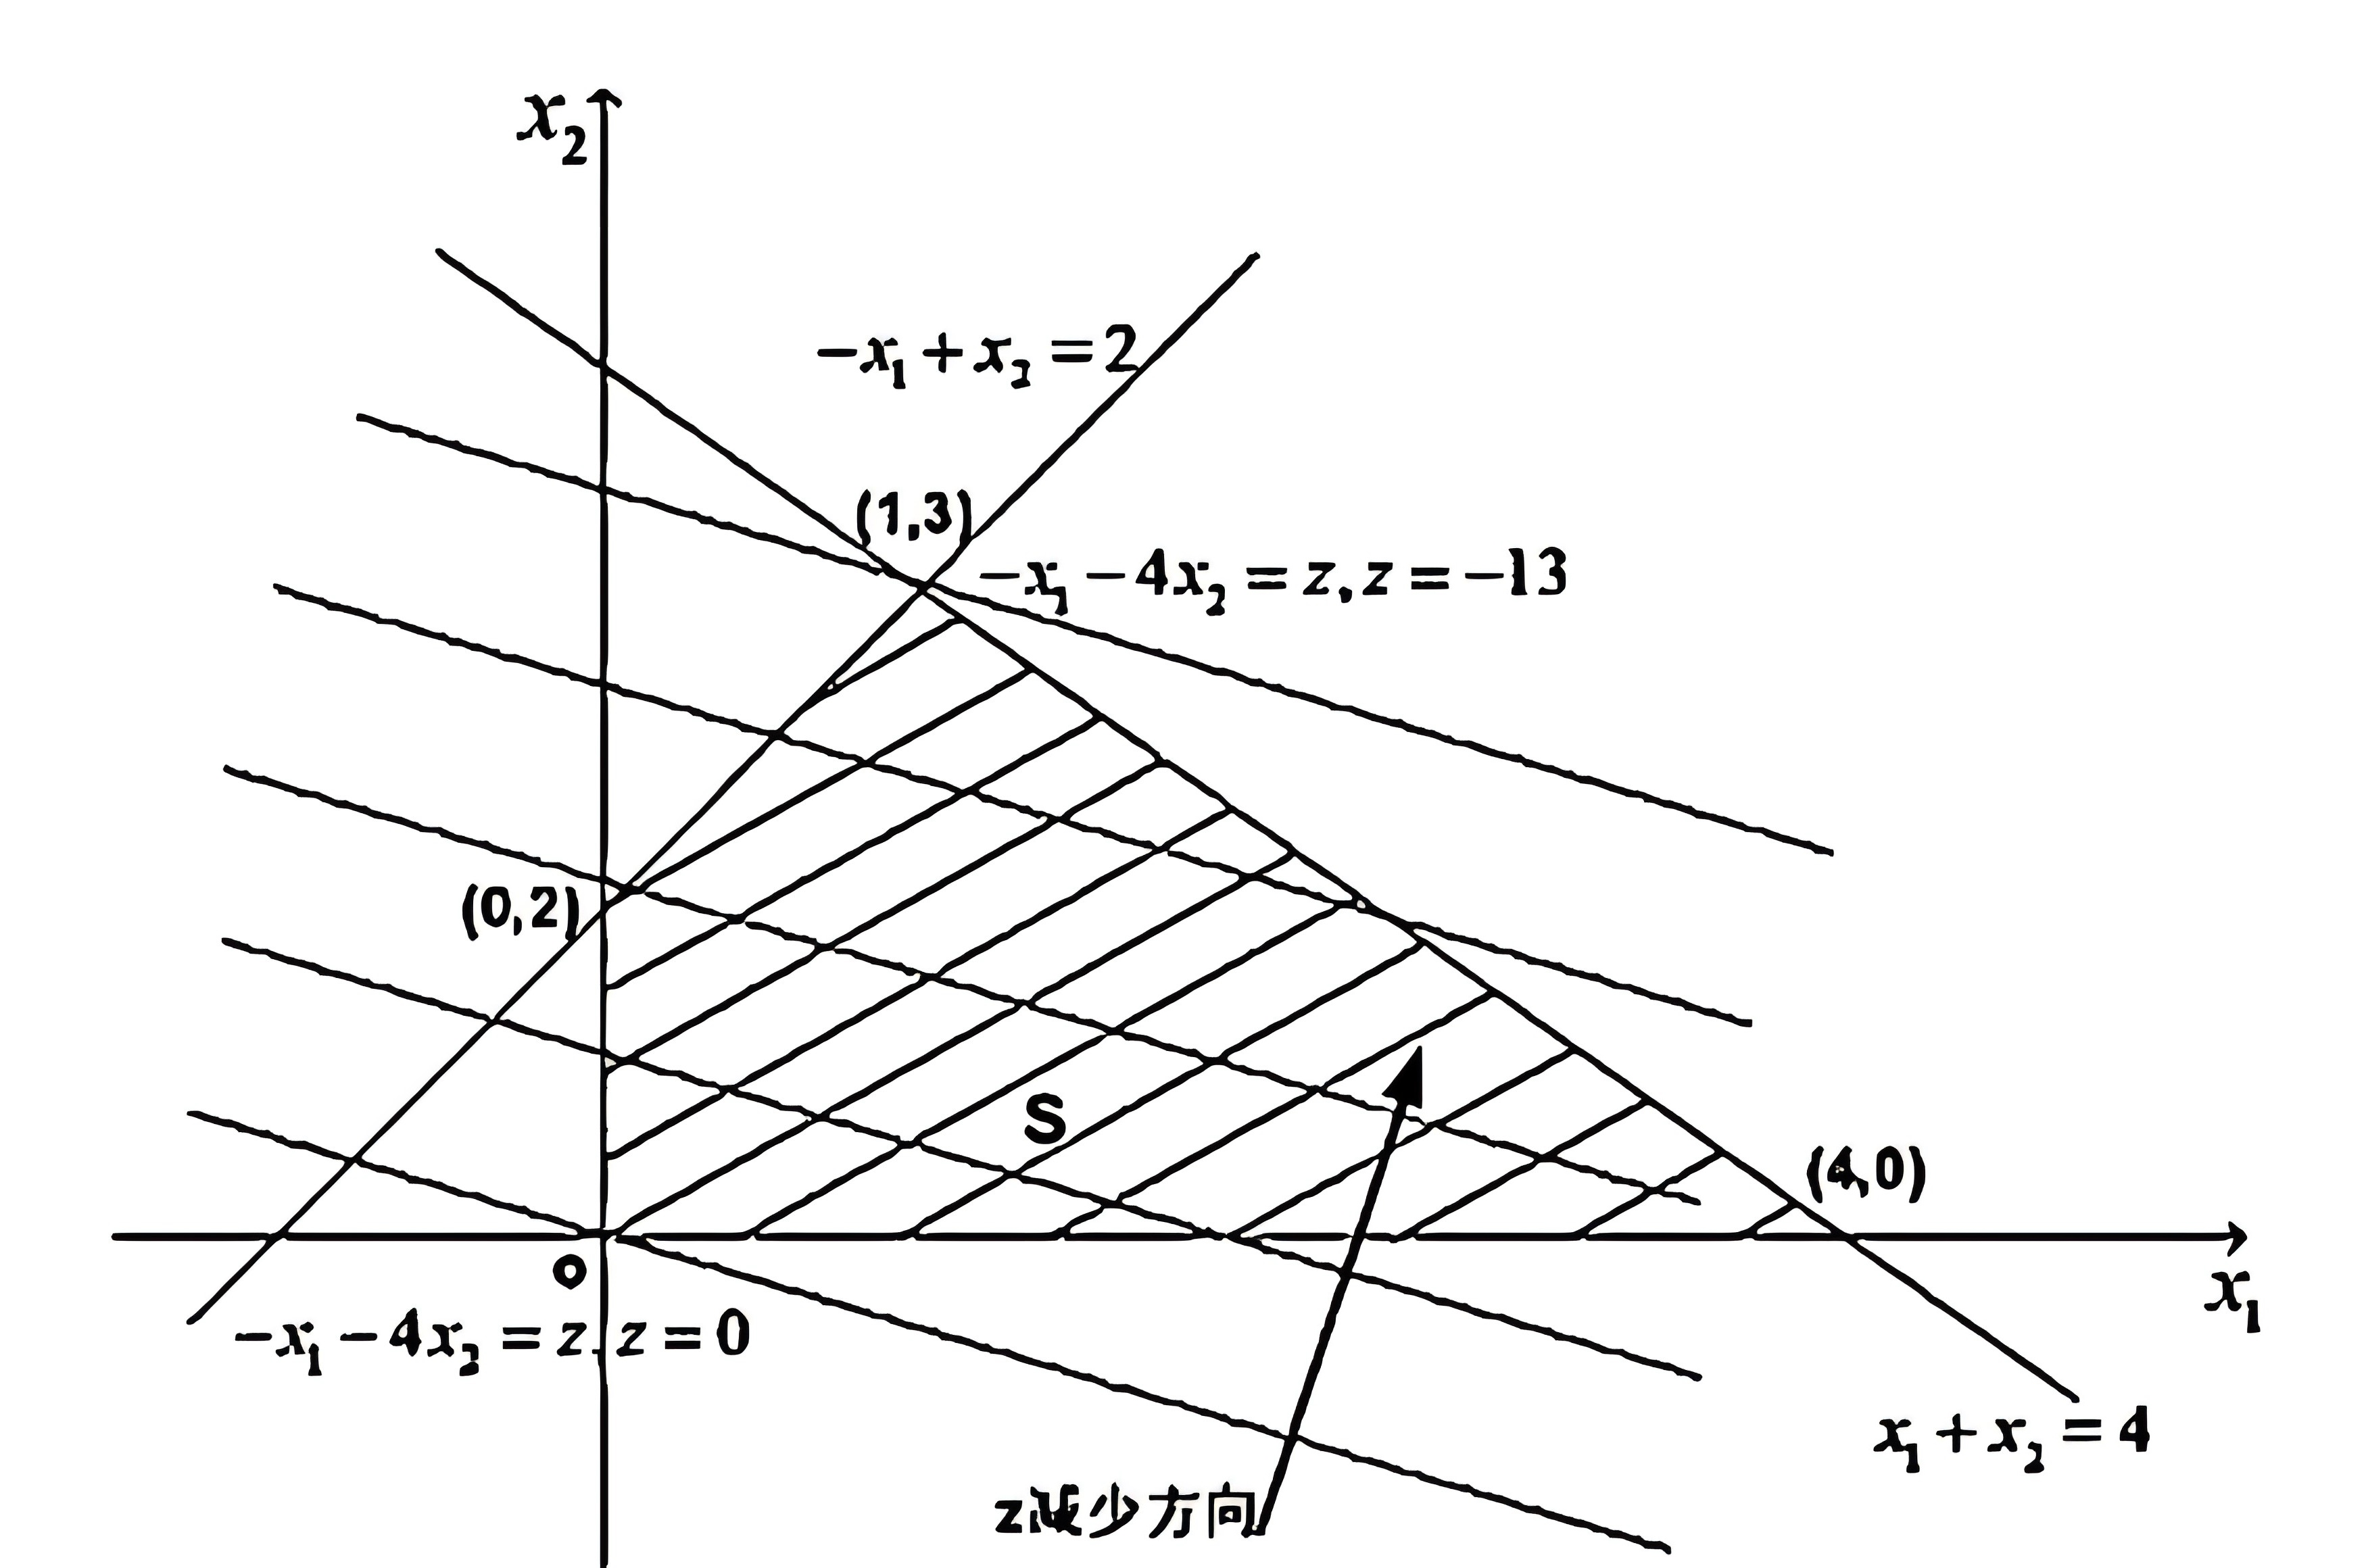
\includegraphics[width=0.6\textwidth]{1.png}
        \caption{例1.1.3图解}
        \label{fig:Temporary Pavilion}
    \end{figure}
    思考:
    \begin{itemize}
        \item \textbf{无穷多解}:上例中若取 $\min z = 3x_1 + 3x_2$ ,则目标函数线与 $x_2 + x_2 = 4$ 边界线重合,带来无穷多解。
        \begin{figure}[H]
            \centering
            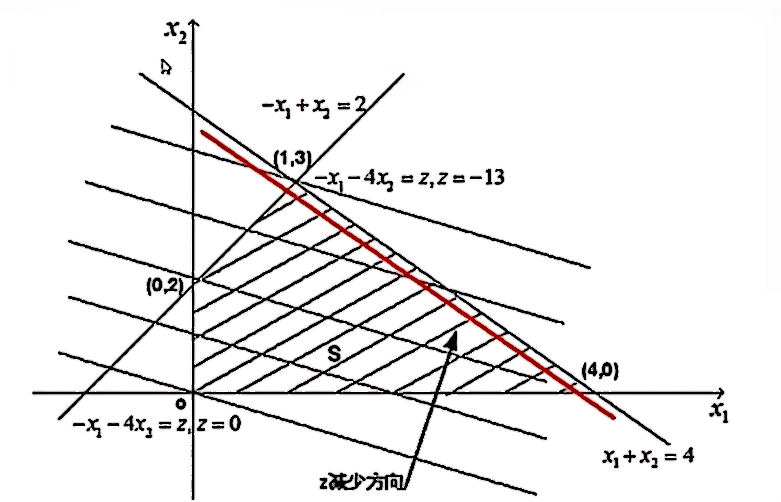
\includegraphics[width=0.4\textwidth]{2.png}
            \label{fig:Temporary Pavilion}
        \end{figure}
        \item \textbf{无界解}:例如下述线性规划问题:
        \begin{align*}
        \max z = x_1 &+ x_2 \\
        \text{s.t.} \quad  -2x_1 + x_2 & \leq 4 \\
         x_1 - x_2 & \leq 2 \\
         x_1, x_2 & \geq 0
        \end{align*}
        \begin{figure}[H]
            \centering
            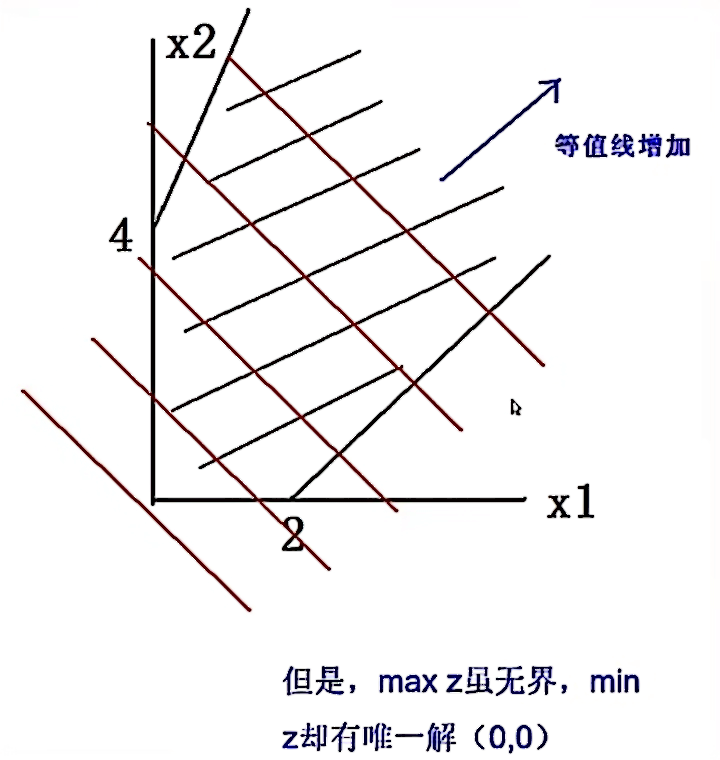
\includegraphics[width=0.4\textwidth]{3.png}
            \label{fig:Temporary Pavilion}
        \end{figure}
        \item \textbf{无最优解}:若可行域为空,则无可行解,自然无最优解。
    \end{itemize}


    \section{线性规划问题的数学模型}
    \begin{thmbox}{一般形式}{cool}
        特点:\textbf{目标函数}和\textbf{约束条件}都是决策变量的线性函数。
        \tcblower
        $\max(\min)\ z= \mathop{\sum}\limits_{j = 1}^{n}{c}_{j}{x}_{j}$\\
        s.t. $\begin{cases} \mathop{\sum }\limits_{j = 1}^{n}{a}_{ij}{x}_{j} \leq(\geq,=){b}_{i}\; & \left( {i = 1,2,\cdots ,m}\right) , \\  {x}_{j} \geq  0 & \left( {j = 1,2,\cdots ,n}\right) . \end{cases}$\\
        \\
        也可以表示为矩阵形式:\\
        $\max(\min)\ z = \mathbf{c}\cdot\mathbf{x}$\\
        s.t. $\begin{cases}\mathbf{A}\mathbf{x}\leq(\geq,=)\mathbf{b}, \\ \mathbf{x}\geq 0\end{cases}$\\
        其中称 $\mathbf{c} = \left( {{\mathrm{c}}_{1},{\mathrm{c}}_{2},\cdots ,{\mathrm{c}}_{\mathrm{n}}}\right)$ 为目标函数的\textbf{系数向量};\\
        称 $\mathbf{x} = {\left( {\mathrm{x}}_{1},{\mathrm{x}}_{2},\cdots ,{\mathrm{x}}_{\mathrm{n}}\right) }^{\mathrm{T}}$ 为\textbf{决策向量};\\
        称 $\mathbf{b} = \left( {{\mathrm{b}}_{1},{\mathrm{\;b}}_{2},\cdots ,{\mathrm{b}}_{\mathrm{m}}}\right)$ 了为约束方程组的\textbf{常数向量};\\
        称 $\mathbf{A} = {\left( {\mathrm{a}}_{\mathrm{{ij}}}\right) }_{\mathrm{m} \times  \mathrm{n}}$ 为约束方程组的\textbf{系数矩阵}; \\
        称 ${p}_{j} = {\left( {a}_{1j},{a}_{2j},\cdots ,{a}_{mj}\right) }^{T}$ 为约束方程组的\textbf{系数向量}.\\
    \end{thmbox}
    
    \begin{thmbox}{标准形}{cool}
        为了便于研究,规定线性规划模型的标准型。
        \tcblower
        $\max\ z = \mathbf{c}\cdot\mathbf{x}$\\
        s.t. $\begin{cases}\mathbf{A}\mathbf{x}=\mathbf{b}, \\ \mathbf{x}\geq 0\end{cases}$\\
    \end{thmbox}
    
    \begin{notebox}{\textbf{方法:一般形式化为标准形的方法}}
    \begin{itemize}[noitemsep]
        \item \textbf{目标函数}:若目标函数为$\min z$,则令$z'=-z$转化为$\max z'$。
        \item \textbf{约束条件}:若约束条件为不等式,可以再不等号左端加上/减去一个非负变量(称为\textbf{松弛变量})化为等式约束(哪边小,加哪边)。
        \item \textbf{决策变量}:若决策变量非正($x_j\leq 0$),则令$x_j'=-x_j$,$x_j'\geq 0$,转化为非负变量。
    \end{itemize}
    \end{notebox}

    \begin{exbox}{一般形式化标准形}{coolexample}
        \begin{align*}
            \min z = x_1 + 2x_2 &- 3x_3 \\
            x_1 + x_2 + x_3 &\leq 7 \\
            x_1 + x_2 + x_3 &\geq 2 \\
            - 3x_1 + x_2 + 2x_3 &= 5 \\
            x_1, x_2 &\geq 0
        \end{align*}
        化为标准形式。\\
        解:
        \begin{enumerate}
            \item 因 $x_3$ 无约束,令 $x_3 = x_4 - x_5,\;x_4,x_5\geq 0$
            \item $x_1 + x_2 + x_3 <  = 7 \rightarrow x_1 + x_2 + (x_4 - x_5) + \textcolor{red}{x_6} = 7$
            \item $x_1 + x_2 + x_3 >  = 2 \rightarrow x_1 + x_2 + (x_4 - x_5) = 2 + \textcolor{red}{x_7}$
            \item $- 3 x_1 + x_2 + 2 x_3 = 5 \rightarrow - 3 x_1 + x_2 + 2\left( {{x}_4 - {x}_5}\right) = 5$
            \\其中:$x_1,x_2,x_4,x_5,x_6,x_7>=0$
        \end{enumerate}
        此时再考虑目标函数\\
        $\min z=-x_1+2x_2-3x_3 \rightarrow \max z'=-z=-x_1-2x_2-3x_4+3x_5+0x_6+0x_7$
    \end{exbox}




    \section{线性规划解的基本概念与基本理论}
    \label{2.3}
    \subsection{解}
    \begin{dfnbox}{可行解}{amznotes}
        满足Theorem 2.2.2约束条件的解$\mathbf{x}=(x_1,x_2,\cdots,x_n)^T$为线性规划问题的\textbf{可行解}。
    \end{dfnbox}
    \begin{dfnbox}{可行域}{amznotes}
        可行解全体构成的集合称为\textbf{可行域},记为$D$。
    \end{dfnbox}
    \begin{dfnbox}{最优解}{amznotes}
        使Theorem 2.2.2中目标函数达到最大的可行解称为\textbf{最优解}。
    \end{dfnbox}

    \subsection{基}
    \begin{dfnbox}{基}{amznotes}
        设系数矩阵 $A = {\left( {a}_{ij}\right) }_{m \times  n}$ 的秩为 $m$ ,则称 $A$ 的某个 $m \times  m$ 非奇
    异子矩阵 $B$ 为线性规划问题的一个\textbf{基}。
    \end{dfnbox}
    不妨设 $B = {\left( {a}_{y}\right) }_{m \times  m} = \left( {\mathbf{p}}_{1},{\mathbf{p}}_{2},\cdots ,{\mathbf{p}}_{m}\right)$ \\
    \begin{itemize}
    \item \textbf{基向量}:向量 ${\mathbf{p}}_{j} = {\left( {a}_{1j},{a}_{2j},\cdots ,{a}_{mj}\right) }^{\mathrm{T}}\left( {j = 1,2,\cdots ,m}\right)$;
    \item \textbf{非基向量}:矩阵 $A$ 的其他列向量;
    \item \textbf{基变量}:与基向量对应的决策变量 ${\mathbf{x}}_{j}\left( j = 1,2,\cdots ,m \right)$;
    \item \textbf{非基变量}:其他的变量称为非基变量。
    \end{itemize}
    
    \subsection{基解}
    设问题的基为$B = \left( {\mathbf{p}}_{1},{\mathbf{p}}_{2},\cdots ,{\mathbf{p}}_{m}\right)$,将约束为:
    \begin{equation}
        \label{eq:2.1}
        \sum_{j=1}^{m} \mathbf{p}_{j}x_{j}=\mathbf{b} - \sum_{j=m+1}^{n} \mathbf{p}_{j}x_{j}
    \end{equation}
    \begin{dfnbox}{基解}{amznotes}
        在方程组 \hyperref[eq:2.1]{(2.1)} 的解中,令$x_j=0(j= m+1, m+2, \cdots , n)$,则解向量 
        \(\mathbf{x} = (x_{1}, x_{2}, \cdots, x_{n}, \cdots, 0, 0)\) 为问题的\textbf{基解}。
    \end{dfnbox}
    \begin{dfnbox}{基可行解、可行基}{amznotes}
        满足非负约束条件的基解称为\textbf{基可行解},对应于基可行解的基解为\textbf{可行基}。
    \end{dfnbox}

    \begin{notebox}{\textbf{方法:理解上述定义}}
        对于$A\mathbf{x}=\mathbf{b}$这样一个矩阵方程,我们以下面为例
        \[
            A = \begin{bmatrix}
            a_{11} & \textcolor{red}{a_{12}} & \textcolor{red}{a_{13}} & \textcolor{red}{a_{14}} & \textcolor{red}{a_{15}} & \textcolor{red}{a_{16}} & a_{17} \\
            a_{21} & \textcolor{red}{a_{22}} & \textcolor{red}{a_{23}} & \textcolor{red}{a_{24}} & \textcolor{red}{a_{25}} & \textcolor{red}{a_{26}} & a_{27} \\
            a_{31} & \textcolor{red}{a_{32}} & \textcolor{red}{a_{33}} & \textcolor{red}{a_{34}} & \textcolor{red}{a_{35}} & \textcolor{red}{a_{36}} & a_{37} \\
            a_{41} & \textcolor{red}{a_{42}} & \textcolor{red}{a_{43}} & \textcolor{red}{a_{44}} & \textcolor{red}{a_{45}} & \textcolor{red}{a_{46}} & a_{47} \\
            a_{51} & \textcolor{red}{a_{52}} & \textcolor{red}{a_{53}} & \textcolor{red}{a_{54}} & \textcolor{red}{a_{55}} & \textcolor{red}{a_{56}} & a_{57}
            \end{bmatrix}
            \quad
            \text{and}
            \quad
            \mathbf{x} =
            \begin{bmatrix}
            x_1 \\
            \textcolor{red}{x_2} \\
            \textcolor{red}{x_3} \\
            \textcolor{red}{x_4} \\
            \textcolor{red}{x_5} \\
            \textcolor{red}{x_6} \\
            x_7\\
            \end{bmatrix}
            \]
        观察,不难发现以下几个性质:
        \begin{itemize}
            \item $A$是一个$m \times n$的矩阵,其中$m<n$,这样决策变量才有多解;如果$m=n$即满秩,就只有唯一解了。
            \item 在矩阵$A$中选取一个$m \times m$的子矩阵$B$,并且这个子矩阵是非奇异的,那么就可以得到一个基,如标红所示。该子矩阵的m个行向量线性无关,m个列向量也线性无关。因此相当于一个m维空间中的坐标系。
            \item 基$B$中的每一个列向量就是基向量,不属于$B$但在$A$中的列向量就是非基向量。
            \item $A$右乘列向量$\mathbf{x}$,$\mathbf{x}$中标红的变量就是与基向量对应的决策变量,其他未标红的变量就是非基变量。
            \item 把基变量留下来,把非基变量移到等式右侧,令非基变量为0,得到的解就是基解;也就是将基$B$中的列向量与$\mathbf{x}$中的基变量相乘,得到的就是基解。换句话说,令$\mathbf{x}$中的非基变量为0,左乘$A$就可以得到基解;
            \item 如果基解本身均大于0,就是基可行解。
        \end{itemize}
    \end{notebox}
    \begin{dfnbox}{凸集}{amznotes}
        假设K为n维欧氏空间中的点集,如果对于任意两点,其连线上所有点均在K内,则称K为\textbf{凸集}。
    \end{dfnbox}
    例:实心圆、实心球是凸集,空心圆、空心球不是凸集。直观地说,凸集没有凹入部分。\\
    \begin{dfnbox}{凸集的顶点}{amznotes}
        对于凸集 $K$ 中的点 $x$,如果 $x$ 不能用相异的两点 $x^{(1)}, x^{(2)} \in K$ 的凸组合表示为
$x = \lambda x^{(1)} + (1 - \lambda) x^{(2)} \in K$ \quad $(0 \leq \lambda \leq 1)$。则称$x$为凸集K的一个顶点
    \end{dfnbox}
    对于凸集,顶点一般为边界点,但并非所有边界点都是顶点.
    

    \subsection{线性规划的几个重要定理}
    基于~\ref{2.3}节中代数学中求解方程和集合论的铺垫之后,我们可以得到几个z重要定理:
    \begin{thmbox}{定理}{cool}
        \begin{enumerate}
            \item 如果线性规划问题存在可行域 $D$,则其可行域 $D = \left\{ x \left| \; \sum_{j=1}^n \mathbf{p}_j x_j = \mathbf{b}, x_j \geq 0 \right. \right\}$ 一定是凸集。
            \item 线性规划问题(2.5),(2.6)的任一个基可行解$\mathbf{x}$必对应于可行域$D$的一个顶点。
            \item 对于可行域
            \begin{itemize}
                \item 如果可行域有界,则问题的最优解一定在可行域的顶点上达到。
                \item 如果可行域无界,则问题可能无最优解;若有最优解也一定在可行域的某个顶点上达到。
            \end{itemize}
        \end{enumerate}
    \end{thmbox}
        定理1的好处在于,凸集有很多良好的性质。\\
        定理2对我们求解没有太大帮助。\\
        定理3将求解最优化的可行域中无穷可解点的比较问题变成了三个定点的比较问题。\\
        \begin{figure}[H]
            \centering
            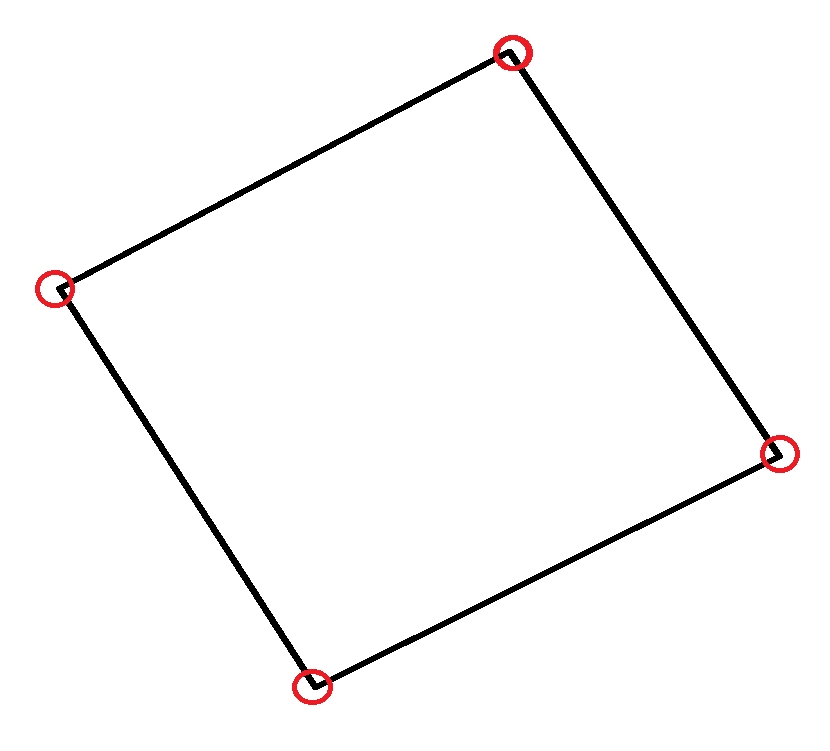
\includegraphics[width=0.6\textwidth]{4.png}
            \caption{例如我们的可行域是上图中的这个四边形,最优解一定在这个四边形的四个顶点上,其他的可行域的点全都不必算。这样我们把无穷维(有无穷个点)的优化问题转化为有限的、可穷举的优化问题。}
            \label{fig:Temporary Pavilion}
        \end{figure}
        总结来说,可以得到四个结论:
        \begin{enumerate}
            \item 线性规划所有可行解构成的集合为\textcolor{red}{凸集},也可能是\textcolor{red}{无界域};
            \item 线性规划的可行域有\textcolor{red}{有限}个顶点;
            \item 线性规划的每个基可行解对应可行域的\textcolor{red}{一个顶点};
            \item 若线性规划有最优解,必定在\textcolor{red}{某个顶点}上达到,但\textbf{并非只能在顶点上达到}。\\
            (比如一个函数在某处有最大值,不是说只有在这一处能达到最大值,可能$f(x_1)=f(x_2)=f_{max},x_1\neq x_2$)
        \end{enumerate}
        本质上可以理解为\textbf{一个可行域内的点,只有顶点是线性无关的,其他任何点都可以由顶点线性表示}。\\
        这些结论构成了单纯形法的理论基础。
    \section{线性规划求解的单纯形法}
    \label{2.4}
    \begin{notebox}{求解线性规划问题的方法}
        \begin{enumerate}
            \item 求一个基可行解(即对应可行域的一个顶点);
            \item 检查该基可行解是否为最优解;
            \begin{itemize}
                \item 如果不是,则设法再求另一个没有检查过的基可行解(可行域内另一个顶点),如此进行下去,直到得到某一个基可行解为最优解为止;
                \item 如果是,结束。
            \end{itemize}
        \end{enumerate}
    \end{notebox}
    这个过程本质上就是先找到可行域内任意一个顶点,然后跳到其他顶点上,穷举的办法求谁最大。就好像我们在函数中,有许多极大值,但是要都求出来去求最大值。
    如果用函数来类比,~\ref{2.4.1}中所做的就是先找到任意一个极大值点$x_1$,~\ref{2.4.2}中所做的就是利用$x_1$便捷地去找其他极大值点;
    \\那么我们不禁要问:
    \begin{itemize}
        \item 如何求出第一个基可行解?(如何找到$x_1$?)
        \item 如何由一个基可行解过渡到另一个基可行解?(怎么通过$x_1$快速找到其他极大值点?)
        \item 如何判断基可行解是否为最优解?(哪个极大值点是最大值点?)
    \end{itemize}
    解决这些问题的方法称为\textbf{单纯形法}。
    \subsection{初始基可行解的确定}
    \label{2.4.1}
    \begin{notebox}{\textbf{初始基可行解的确定方法}}
        \begin{enumerate}
            \item \textbf{标准化}:第一步,将线性规划模型化为标准型;
            \item \textbf{解方程}:第二步,解矩阵方程,得到基可行解。
        \end{enumerate}
    \end{notebox}
    这一步骤本质上是\textbf{找到可行域的任意一个顶点},且只能硬着头皮算。考虑到读者可能和笔者一样忘记了线性代数的相关内容,因此在这里对矩阵方程解法加以补充:
    现在假设我们有:
    \[
    \quad
    A = \begin{bmatrix}
    1 & 2 & 3 & 4 & 5 \\
    2 & 3 & 4 & 5 & 6 \\
    3 & 4 & 5 & 6 & 7
    \end{bmatrix}, \quad
    \mathbf{x} = \begin{bmatrix}
    x_1 \\
    x_2 \\
    x_3 \\
    s_1 \\
    s_2
    \end{bmatrix}, \quad
    \mathbf{b} = \begin{bmatrix}
    4 \\
    5 \\
    7
    \end{bmatrix}
    \]
    \begin{itemize}
        \item 从系数矩阵 $A = \left( a_{ij} \right)_{m \times n}$  
        $\left( m < n, \text{秩为} m \right)$ 总可以得到一个 $m$ 阶单位阵 $E_{m}$ 。(例如,可以通过  
        高斯消元法对系数矩阵 $A$ 进行行初等变换,得到一个 $m$ 阶单位阵 $E_{m}$ )。  
        $A\mathrm{x} = \mathrm{b} \rightarrow \left[ E_{m} \text{ 其他元素} \right] \mathrm{x'} = \mathrm{b'}$.\\

        \[
        A \xrightarrow{\text{初等变换}} \begin{bmatrix}
        \textcolor{red}{1} & \textcolor{red}{0} & \textcolor{red}{0} & -2 & -3 \\
        \textcolor{red}{0} & \textcolor{red}{1} & \textcolor{red}{0} & -3 & -4 \\
        \textcolor{red}{0} & \textcolor{red}{0} & \textcolor{red}{1} & 0 & 0
        \end{bmatrix}
        \]

        \item 取如上 $m$ 阶单位阵 $E_{m}$ 为初始可行基,即 $B = E_{m}$, 将相应的约束方程组变为:  
        ${x}_i = {b}_i - {a}_{i,m + 1}{x}_{m + 1} - \cdots - {a}_{i,n}{x}_n \quad (i = 1, 2, \cdots, m)$.  
        \\
        \[
        \begin{bmatrix}
        \textcolor{red}{1} & \textcolor{red}{0} & \textcolor{red}{0} & -2 & -3 \\
        \textcolor{red}{0} & \textcolor{red}{1} & \textcolor{red}{0} & -3 & -4 \\
        \textcolor{red}{0} & \textcolor{red}{0} & \textcolor{red}{1} & 0 & 0
        \end{bmatrix}
        \times
        \begin{bmatrix}
        \textcolor{red}{x_1} \\
        \textcolor{red}{x_2} \\
        \textcolor{red}{x_3} \\
        \textcolor{blue}{s_1} \\
        \textcolor{blue}{s_2}
        \end{bmatrix}
        =
        \begin{bmatrix}
        4 \\
        5 \\
        7
        \end{bmatrix}
        \]

        \[
        \text{解得列向量:}
        \quad \begin{bmatrix}
        4 \\
        5 \\
        7 \\
        0 \\
        0
        \end{bmatrix}
        \]

        \item 令方程组后面的 $n - m$ 个变量为 0, ${x}_j = 0 \quad (j = m + 1, m + 2, \ldots, n)$,  
        则可得一个初始基可行解: 
        ${x}^{(0)} = \left( {x}_1^{(0)}, {x}_2^{(0)}, \ldots, {x}_m^{(0)}, 0, \ldots, 0 \right)^T = \left( {b}_1, {b}_2, \cdots, {b}_m, 0, \cdots, 0 \right)^T$.\\
        \[
        \text{令非基变量为0:}
        \quad \begin{bmatrix}
        4 \\
        5 \\
        7 \\
        0 \\
        0
        \end{bmatrix}
        \]
    \end{itemize}

    \subsection{寻找另一个基可行解:基变换法}
    \label{2.4.2}
    为了确定在其他顶点上的可行解,我们需要使用\textbf{基变换法}的方法。
    \begin{notebox}{\textbf{基变换法}}    
    \\当一个基可行解不是最优解或不能判断时,需要过渡到另一个基可行解,即从基可行解,
    \[
    \mathbf{x}^{(0)} = \left( x_1^{(0)}, x_2^{(0)}, \ldots, x_m^{(0)}, 0, \ldots, 0 \right)^T
    \]
    对应的可行基 

    \[
    B = \left( p_1, p_2, \ldots, p_m \right)
    \]
    中替换一个列向量,用来替换的列向量与原向量组未被替换的向量线性无关。

    例如,用非基变量 \( p_{m+t} \left( 1 \leq t \leq n - m \right) \) (称为换入变量)替换基变量 \( p_1 \left( 1 \leq 1 \leq m \right) \) (称为换出变量),就可得到一个新的可行基

    \[
    B_1 = \left( p_1, \ldots, p_{1-1}, p_{m+t}, p_{1+1}, \ldots, p_m \right)
    \]
    从而可以求出一个新的基可行解

    \[
    \mathbf{x}^{(1)} = \left( x_1^{(1)}, x_2^{(1)}, \ldots, x_m^{(1)}, 0, \ldots, 0 \right)^T
    \]
    \end{notebox}
    我们仍然用刚才的例子:\\
    \[
    A' = \begin{bmatrix}
    1 & 0 & 0 & -2 & -3 \\
    0 & 1 & 0 & -3 & -4 \\
    0 & 0 & 1 & 0 & 0
    \end{bmatrix}
    \]
    这是初始变换后的矩阵 \( A' \),前三列已经是单位矩阵。

    % 步骤 1:交换第三列和第四列后的矩阵 A''

    \[
    A'' = \begin{bmatrix}
    1 & 0 & \textcolor{pink}{0} & \textcolor{blue}{-2} & -3 \\
    0 & 1 & \textcolor{pink}{0} & \textcolor{blue}{-3} & -4 \\
    0 & 0 & \textcolor{pink}{1} & \textcolor{blue}{0} & 0
    \end{bmatrix}
    \]
    在这个步骤中,我们交换了 \( A' \) 的第三列和第四列,粉色为换出变量,蓝色为换入变量。

    % 步骤 2:经过初等变换后的矩阵 A'''

    \[
    A''' = \begin{bmatrix}
    1 & 0 & 0 & * & * \\
    0 & 1 & 0 & * & * \\
    0 & 0 & 1 & * & *
    \end{bmatrix}
    \]
通过适当的初等变换(例如对第三列和第四列进行适当的线性组合),我们将前三列转换为单位矩阵,最终得到了这个矩阵。这样我们得到了一个新的可行基,以此可以继续解方程得到另一个可行解。\\
当然,也有可能换入非基变量后,我们应该首先检查更换后的“基”是否可逆,比如发现新的三个列向量线性相关而不是线性无关,不能构成一个基,那么此时应该换一个非基变量换入。
\begin{thmbox}{线性规划模型的另一个基可行解}{cool}
    事实上,这个新的基可行解可以用以下公式直接计算出来:
    \[
    \mathbf{x}_i^{(1)} = \left\{
    \begin{matrix}
    \mathbf{x}_i^{(0)} - \theta \beta_{i, m+t}, & i \neq l \\
    \theta, & i = l
    \end{matrix}
    \right.
    \quad
    \left( \begin{matrix}
    i = 1, 2, \cdots, m, \\
    1 \leq l \leq m, 1 \leq t \leq n - m
    \end{matrix} \right)
    \]
    其中
    \[
    \theta = \frac{\mathbf{x}_i^{(0)}}{\beta_{i, m+t}} = \min\limits_{1 \leq i \leq m} \left\{ \frac{\mathbf{x}_i^{(0)}}{\beta_{i, m+t}} \mid \beta_{i, m+t} > 0 \right\},
    \]
    并且
    \[
    \mathbf{p}_{m+t} = \sum\limits_{i=1}^{m} \beta_{i, m+t} \mathbf{p}_i.
    \]
    如果 \( \mathbf{x}^{(1)} = \left( \mathbf{x}_1^{(1)}, \mathbf{x}_2^{(1)}, \ldots, \mathbf{x}_m^{(1)}, 0, \ldots, 0 \right)^T \) 仍不是最优解,则可以重复利用这种方法,直到得到最优解为止。
\end{thmbox}
    \subsection{最优性检验方法}
    实际上,我们并不需要把所有的“顶点”都找到再去比较哪个最大。我们可以找到可行域中的\textbf{任意一点},因为这个点是不独立的(可以由其他所有顶点线性表示),
    所以如果我们找到了一个顶点$x_1$,得到目标函数值$z_1=cx_1$;而有任一点$x=a_1x_1+a_2x_2+\cdots+a_nx_n$,
    得到目标函数值$z=cx$。只需要比较$z_1$和$z$,即可知道$z_1$是否是最大值,证明过程如下(感兴趣的同学可以了解):\\
    将基可行解 \( \mathbf{x}^{(1)} \) 和这个任意的 \( \mathbf{x} = \left( x_1, x_2, \ldots, x_n \right)^T \) 分别代入目标函数得:
    \[
    z^{(1)} = \sum_{i=1}^{m} c_i x_i^{(1)} = \sum_{i=1}^{m} c_i b_i^{\prime}, \psi
    \]

    \[
    z = \sum_{i=1}^{n} c_i x_i = \sum_{i=1}^{m} c_i x_i + \sum_{i=m+1}^{n} c_i x_i
    \]

    \[
    = \sum_{i=1}^{m} c_i \left( b_i^{\prime} - \sum_{j=m+1}^{n} a_{ij}^{\prime} x_j \right) + \sum_{j=m+1}^{n} j j^+ j
    \]

    \[
    = \sum_{i=1}^{m} c_i b_i^{\prime} + \sum_{j=m+1}^{n} \left( c_j - \sum_{i=1}^{m} c_i a_{ij}^{\prime} \right) x_j^{\prime}
    \]

    \[
    = z^{(1)} + \textcolor{red}{\sum_{j=m+1}^{n} \left( c_j - z_j \right) x_j}
    \]

    其中 \( z_j = \sum_{i=1}^{m} c_i a_{ij}^{\prime} \quad (j = m+1, \cdots, n) \)。 记 \( \sigma_j = c_j - z_j \quad (j = m+1, \cdots, n) \),则

    \[
    z = z^{(1)} + \textcolor{red}{\sum_{j=m+1}^{n} O_j x_j} \quad \
    \]
    注意到:
    当 \( \sigma_j > 0 \quad (j = m+1, \cdots, n) \) 时,就有

    \[
    z > z^{(1)} ;
    \]
    当 \( \sigma_j \leq 0 \quad (j = m+1, \cdots, n) \) 时,就有

    \[
    z \leq z^{(1)}.
    \]

    为此,\( \sigma_j = c_j - z_j \) 的符号是判别 \( \mathbf{x}^{(1)} \) 是否为最优解的关键所在,故称之为\textcolor{red}{检验数}。于是可以得出下面的结论:
    \begin{notebox}{\textbf{判断最优解的办法}}    
        \\
        \begin{enumerate}
            \item 如果 \( \sigma_j \leq 0 \quad (j = m+1, \cdots, n) \),则 \( \mathbf{x}^{(1)} \) 是问题的最优解,最优值为 \( z^{(1)} \);
            \item 如果 \( \sigma_j \leq 0 \quad (j = m+1, \cdots, n) \),且至少存在一个 \( \sigma_{m+k} = 0 \quad (0 \leq k \leq n-m) \),
            则问题有无穷多个最优解,\( \mathbf{x}^{(1)} \) 是其中之一,最优值为 \( z^{(1)} \);
            \item 如果 \( \sigma_j < 0 \quad (j = m+1, \cdots, n) \),则 \( \mathbf{x}^{(1)} \) 是问题的唯一最优解,最优值为 \( z^{(1)} \);
            \item 如果存在某个检验数 \( \sigma_{m+k} > 0 \quad (0 \leq k \leq n-m) \),并且对应的系数向量 \( \mathbf{p}_{m+k} \) 的各分量
            \( a_{i, m+k} \leq 0 \quad (i = 1, 2, \cdots, m) \),则问题具有无界解(即无最优解)。
        \end{enumerate}
    \end{notebox}
    
    ~\ref{2.4}\textbf{节所有上述所有过程一般上不需要我们了解的过于深入,因为有现成的计算机函数可以用,但是可以领会其思想。}


    \section{线性规划问题的灵敏度分析}
    在线性规划模型
    \[
    \max z = \mathbf{c} \cdot \mathbf{x}
    \]
    约束条件为

    \[
    \left\{
    \begin{array}{l}
    \mathbf{A} \mathbf{x} = \mathbf{b} \\
    \mathbf{x} \geq \mathbf{0}
    \end{array}
    \right.
    \]
    其中,总假设 \( \mathbf{A}, \mathbf{b}, \mathbf{c} \) 都是常数,但这些数值在许多情况下是由试验或测量得到的,特别是在迭代计算中,这些数值都是近似值。通常,\( \mathbf{A} \) 表示工艺条件,\( \mathbf{b} \) 表示资源条件,\( \mathbf{c} \) 表示市场条件。在实际中,可能有多种原因引起它们的变化。

    现在的问题是:这些系数在什么范围内变化时,线性规划问题的最优解不发生变化?这就是灵敏度分析要研究的问题。\\
    \textbf{这一问题比较复杂,本课程不做深入探究,但是大作业可以考虑}



    \section{应用案例分析}
    \subsection{下料问题}
    \begin{exbox}{下料问题}{coolexample}
        某单位需要加工作 100 套工架,每套工架需用长为 2.9m,2.1m 和1.5m 的圆钢各一根,已知原材料长 7.4m,现在的问题是如何下料使得所用的原材料最省?
        \\
        \\
        解:
        简单分析,在每一根原材料上各截取一根 2.9m,2.1m 和 1.5m的圆钢做成一套工架,每根原材料剩下料头 0.9m。要完成 100 套工架,就需要用 100 根原材料,共剩余 90m 料头。
        \\若采用套截方案,则可以节省原材料。下面给出了几种可能的套截方案,如表2.1所示。\\
        实际上,为了保证完成这100套工架,使所用原材料最省,可以混合使用各种下料方案。\\
        设按方案 \( A, B, C, D, E \) 下料的原材料数分别为 \( x_1, x_2, x_3, x_4, x_5 \)。根据表格 2-1,可以得到如下线性规划模型。
        目标函数:

        \[
        \min z = 0x_1 + 0.1x_2 + 0.2x_3 + 0.3x_4 + 0.8x_5
        \]

        约束条件:

        \[
        \begin{cases}
        x_1 + 2x_2 + x_4 = 100 \\
        2x_3 + 2x_4 + x_5 = 100 \\
        3x_1 + x_2 + 2x_3 + 3x_5 = 100 \\
        x_1, x_2, x_3, x_4, x_5 \geq 0
        \end{cases}
        \]
        所有 \( 2.9 \) 的料总数 100,所有 \( 2.1 \) 的料总数 100,所有 \( 1.5 \) 的料总数 100。
    \end{exbox}

    \begin{table}[H]  % 使用 H 强制放置位置
        \centering
        \renewcommand{\arraystretch}{1.5} % 调整行高
        \begin{tabular}{|c|c|c|c|c|c|}
        \hline
        \multirow{2}{*}{长度/m} & \multicolumn{5}{c|}{方案} \\ \cline{2-6} 
         & A & B & C & D & E \\ \hline
        2.9 & 1 & 2 & 0 & 1 & 0 \\ \hline
        2.1 & 0 & 0 & 2 & 2 & 1 \\ \hline
        1.5 & 3 & 1 & 2 & 0 & 3 \\ \hline
        合计/m & 7.4 & 7.3 & 7.2 & 7.1 & 6.6 \\ \hline
        料头/m & 0 & 0.1 & 0.2 & 0.3 & 0.8 \\ \hline
        \end{tabular}
        \caption{例2.6.1下料方案}
    \end{table}
        
        \begin{codebox}{MATLAB代码}{线性规划求解}
            \begin{amzcode}{matlab}
                c = [0, 0.1, 0.2, 0.3, 0.8]';
                b1 = [0, 0, 0, 0, 0]';
                b2 = [100, 100, 100]';
                A1 = [-1, 0, 0, 0, 0; 0, -1, 0, 0, 0; 0, 0, -1, 0, 0; 0, 0, 0, -1, 0; 0, 0, 0, 0, -1]';
                A2 = [1, 2, 0, 1, 0; 0, 0, 2, 2, 1; 3, 1, 2, 0, 3]';
                [x, fv] = linprog(c, A1, b1, A2, b2);
            \end{amzcode}
        \end{codebox}
        
        运行该程序后,立即可以得到最优解为 $\mathbf{x}=(12.8243\text{,}27.1757\text{,}17.1757\text{,}32.8243\text{,}0)^{\mathrm{T}}$。四舍五入的方法取整得
        $\mathbf{x}=(13,27\text{,}17\text{,}33\text{,}0)^{\mathrm{T}}$。最优值为$z=16$,即接方案 A 下料 13 根,方案B下料 27 根,方案 c下料 17 根,方案 D 下料 33 根,共需原材料 90 根就可以制作完成 100 套工架,剩余料头最少为 16m。

        \begin{notebox}{\textbf{matlab代码解析}}
            \begin{enumerate}
                \item \textbf{目标函数定义}:\\
                \texttt{c = [0, 0.1, 0.2, 0.3, 0.8]'} 定义了最小化料头长度的目标函数系数向量,对应五种下料方案的料头长度。
            
                \item \textbf{约束条件设置}:
                \begin{itemize}
                    \item \texttt{b1 = [0, 0, 0, 0, 0]'} 设置变量非负约束的右端项
                    \item \texttt{b2 = [100, 100, 100]'} 设置三种圆钢需求量的右端项
                    \item \texttt{A1} 矩阵通过负单位矩阵实现 $x_i \geq 0$ 的非负约束
                    \item \texttt{A2} 矩阵的每一列对应一个下料方案:
                    \begin{itemize}
                        \item 第一行:2.9m圆钢的生产数量约束
                        \item 第二行:2.1m圆钢的生产数量约束
                        \item 第三行:1.5m圆钢的生产数量约束
                    \end{itemize}
                \end{itemize}
            
                \item \textbf{线性规划求解}:\\
                \texttt{linprog(c, A1, b1, A2, b2)} 调用MATLAB线性规划求解器,其中:
                \begin{itemize}
                    \item 输入参数:目标系数 \texttt{c},不等式约束 \texttt{A1, b1},等式约束 \texttt{A2, b2}
                    \item 输出参数:\texttt{x} 为最优解向量,\texttt{fv} 为最优目标值
                \end{itemize}
            
                \item \textbf{结果修正}:\\
                原始解包含小数,通过四舍五入得到整数解 \texttt{(13,27,17,33,0)},此时总用料90根,剩余料头16m。
            \end{enumerate}
        \end{notebox}
        
        
        \begin{codebox}{LINGO代码}{线性规划模型}
            \begin{amzcode}{matlab}
                MODEL
                sets;
                row/1 2 3/:b;
                arrange/1..5/:x c;
                endsets;

                data:
                b=100,100,100;
                c=0 0 1 0.2 0 3 0.8.
                a=1,2,0,1,0,0,0,2,2,1 3,1 2,0,3;
                enddata.

                [oBJ] min=@sum(arrange(j):c(j)*x(j));
                @for(row(i):@sum(arrange(j);a(lj)*x(j))=b(i););
                @for(arrange(j);x(j)>=0;);
                END
            \end{amzcode}
        \end{codebox}
        
        运行该程序后,立即可以得到最优解为 $\mathbf{x}=(0\text{,}40\text{,}30\text{,}20\text{,}0)^{\mathrm{T}}$,最优值为 $z=16$,即按方案 B下料 40 根,方案C下料 30 根,方案 D 下料 20 根,共需原材料 90根就可以制作完成 100 套工架,剩余料头最少为 16m。

        \subsection{连续投资问题}
        
        \begin{exbox}{连续投资问题}{coolexample}
            某投资公司拟制定今后5年的投资计划,初步考虑下面的四个投资项目:
            \\项目A:从第1年到第4年每年年初需要投资,于次年年末收回成本,并可获利润 15\%;。
            \\项目 B:第3年年初需要投资.到第5年年末可以收回成本,并获得利润 25\%但为了保证足够的资金流动,规定该项目的投资金额上限为不超过总金额的40%;
            \\项目C:第2年年初需要投资,到第5年年来可以收回成本,并获得利润 40\%,
            但规定该项目的最大投资金额不超过总金额的 30\%;
            \\项目D:5年内每年年初可以购买公债,于当年年末可以归还本金,并获利息 6\%。
            \\该公司现有投资金额 100万元,请你帮助该公司制定这些项目每年的投资计划,使公司到第5年年末能够获得最大的利润。
            \\
            \\
            解:
            虽然这是一个连续投资问题,即属于动态优化问题,但是在这里可以用静态优化的方法来解决。用决策变量分别表示第i年年初为项目 A,B,C,D的投资额,根据问题的要求各变量的对应关系如表2-7所示(表格待补充),表中空白处表示当年不能为该项目投资,也可认为投资额为0。\\
            \\
            首先注意到,项目 \(D\) 每年都可以投资,并且当年末就能收回本息,所以公司每年应把全部资金都投出去。因此,投资方案应满足下面的条件。
            第 1 年:将 100 万元资金全部用于项目 \(A\) 和项目 \(D\) 的投资,即:

            \[
            x_{11} + x_{14} = 1000000
            \]
            第 2 年:因为第 1 年用于项目 \(A\) 的投资到第 2 年年末才能收回,所以能用于第 2 年年初的投资金额只有项目 \(D\) 的第 1 年收回的本息总额 \(x_{14}(1 + 0.06)\)。于是第 2 年的投资分配为:

            \[
            x_{21} + x_{23} + x_{24} = 1.06 x_{14}
            \]

            于是可以得到问题的线性规划模型为:

            \[
            \max z = 1.15 x_{41} + 1.25 x_{32} + 1.40 x_{23} + 1.06 x_{54}
            \]
            约束条件如下:

            \[
            \begin{aligned}
            x_{11} + x_{14} &= 1000000 \\
            -1.06 x_{14} + x_{21} &+ x_{23} + x_{24} = 0 \\
            -1.15 x_{11} - 1.06 x_{24} &+ x_{31} + x_{32} + x_{34} = 0 \\
            -1.15 x_{21} - 1.06 x_{34} &+ x_{41} + x_{44} = 0 \\
            -1.15 x_{31} - 1.06  &x_{44} + x_{54} = 0 \\
            x_{32} \leq &400000 \\
            x_{32} \leq &300000 \\
            x_{33} \leq x_{33} &+ x_{44} \leq 0.3 \\
            4 \leq &t \leq 5
            \end{aligned}
            \]
            考虑到这个问题的实际情况,这里使用 LINGO 求解该线性规划模型。

            运行该程序后,得到最优解:

            $
            x_{11} = 716981.1
            ,
            x_{14} = 283018.9
            ,
            x_{23} = 300000
            ,
            x_{31} = 424528.3
            ,
            x_{32} = 400000
            ,
            x_{54} = 488207.5
            $
            
            其他的变量均为零,最优值为:

            \[
            z = 1437500
            \]
            即连续投资方案为:
            \begin{itemize}
                \item 第 1 年用于投资项目 \(A\) 的金额为 716981.1 元,项目 \(D\) 的金额为 283018.9 元。
                \item 第 2 年用于项目 \(C\) 的投资金额为 300000 元。
                \item 第 3 年用于项目 \(A\) 的投资为 424528.3 元,项目 \(B\) 的金额为 400000 元。
                \item 第 5 年用于投资项目 \(D\) 的金额为 488207.5 元。
            \end{itemize}
            到第 5 年年末,该公司拥有总资金为 1437500 元,收益率为 43.75\%。
            \end{exbox}

            
\ifx\allfiles\undefined
	
	% 如果有这一部分的参考文献的话,在这里加上
	% 没有的话不需要
	% 因此各个部分的参考文献可以分开放置
	% 也可以统一放在主文件末尾。
	
	%  bibfile.bib是放置参考文献的文件,可以用zotero导出。
	% \bibliography{bibfile}
	
	end{document}
	\else
	\fi
    \ifx\allfiles\undefined

	% 如果有这一部分另外的package,在这里加上
	% 没有的话不需要
	
	\begin{document}
\else
\fi
\section{第二章作业}
\subsection{配餐问题}
\textbf{Q:编程求解本章ppt中例2.2合理配餐问题,需要的基础数据自拟。}
\\某幼儿园为了保证孩子们的健康成长,要求对每天的膳食进行合理科学的搭配,以保证孩子们对各种
营养的需求.从营养学的角度.假设共有5种食品$A_j$$(j=1,2.…,6)$可供选择,每种食品都含有加6种不同
的营养成分$B_i$$(i=1,2.,6)$.而且每单位的食品$A_j$含有营养成分$B_i$的含量如下表所示(数据为自拟):

\begin{table}[H]
    \centering
    \renewcommand{\arraystretch}{1.5}
    \begin{tabular}{|c|c|c|c|c|c|c|}
    \hline
    \multirow{2}{*}{营养成分} & \multicolumn{5}{c|}{食品} & \multirow{2}{*}{最低需求量} \\ \cline{2-6} 
     & A1 & A2 & A3 & A4 & A5 & \\ \hline
    B1 & 4.0 & 0.4 & 0.8 & 0.5 & 0.9 & 16.0 \\ \hline
    B2 & 0.5 & 4.0 & 0.5 & 0.7 & 0.7 & 26.0 \\ \hline
    B3 & 0.6 & 0.2 & 4.0 & 0.4 & 0.5 & 18.0 \\ \hline
    B4 & 0.7 & 0.1 & 0.3 & 4.0 & 0.3 & 12.0 \\ \hline
    B5 & 0.8 & 0.9 & 0.2 & 0.3 & 4.0 & 14.0 \\ \hline
    B6 & 1.2 & 1.3 & 1.4 & 1.4 & 1.3 & 20.0 \\ \hline
    \textbf{食品单价} & 5 & 6 & 7 & 8 & 9 & \\ \hline
    \textbf{摄入量最小值} & 2.0 & 3.0 & 3.0 & 1.0 & 3.0 & \\ \hline
    \end{tabular}
    \caption{营养数据表}
\end{table}

\begin{enumerate}
    \item 每人每天对营养成分$B_i$的最低需求为$b_i(i=1,2,\dots,6)$,而且食品$A_j$的单价为$c_j(j=1,2,\dots,5)$. 问如何合理科学地制定配餐方案,既可以保证孩子们的营养需求,又使每人每天所需的费用最低?
    \item 除了如上的要求之外,如果还要求各种食品的合理搭配,即要求每人每天对食品$A_j$的摄入量不少于$d_j(j=1,2,\dots,5)$,问配餐方案又如何?
\end{enumerate}

\textbf{A:分析如下。}
\begin{enumerate}
    \item \textbf{基础配餐问题(仅考虑营养需求)}
    \begin{itemize}
        \item \textbf{决策变量}:设每天采购食品 $ A_j $ 的数量为 $ x_j $(单位:份),其中 $ j=1,2,\dots,5 $
        \item \textbf{目标函数}:最小化总费用
        $$
        \min z = 5x_1 + 6x_2 + 7x_3 + 8x_4 + 9x_5
        $$
        \item \textbf{约束条件}:
        \begin{enumerate}
            \item \textbf{营养成分需求}(满足最低摄入量):
            $$
            \begin{cases}
            4.0x_1 + 0.4x_2 + 0.8x_3 + 0.5x_4 + 0.9x_5 \geq 16.0 \quad (\text{营养成分 } B_1) \\
            0.5x_1 + 4.0x_2 + 0.5x_3 + 0.7x_4 + 0.7x_5 \geq 26.0 \quad (\text{营养成分 } B_2) \\
            0.6x_1 + 0.2x_2 + 4.0x_3 + 0.4x_4 + 0.5x_5 \geq 18.0 \quad (\text{营养成分 } B_3) \\
            0.7x_1 + 0.1x_2 + 0.3x_3 + 4.0x_4 + 0.3x_5 \geq 12.0 \quad (\text{营养成分 } B_4) \\
            0.8x_1 + 0.9x_2 + 0.2x_3 + 0.3x_4 + 4.0x_5 \geq 14.0 \quad (\text{营养成分 } B_5) \\
            1.2x_1 + 1.3x_2 + 1.4x_3 + 1.4x_4 + 1.3x_5 \geq 20.0 \quad (\text{营养成分 } B_6) \\
            \end{cases}
            $$
            \item \textbf{非负约束}:
            $$
            x_1, x_2, x_3, x_4, x_5 \geq 0
            $$
        \end{enumerate}
    \end{itemize}
    
    \item \textbf{扩展配餐问题(增加食品摄入量约束)}
    
    \begin{itemize}
        \item \textbf{决策变量}:同上,仍为 $ x_j $
        \item \textbf{目标函数}:同上,仍为最小化总费用
        $$
        \min z = 5x_1 + 6x_2 + 7x_3 + 8x_4 + 9x_5
        $$
        \item \textbf{约束条件}:
        \begin{enumerate}
            \item \textbf{原营养成分需求}:同上
            \item \textbf{食品摄入量下限}(表格中“摄入量最值”):
            $$
            \begin{cases}
            x_1 \geq 2.0 \\
            x_2 \geq 3.0 \\
            x_3 \geq 3.0 \\
            x_4 \geq 1.0 \\
            x_5 \geq 3.0 \\
            \end{cases}
            $$
            \item \textbf{非负约束}:同上
        \end{enumerate}
    \end{itemize}
\end{enumerate}
\begin{codebox}{Matlab代码}{线性规划模型}
    \begin{amzcode}{matlab}
        % 配餐优化:求解浮点数和整数解
        clear; clc;
        
        % 营养含量矩阵 A(6x5,行:B1-B6,列:A1-A5)
        A = [4.0, 0.4, 0.8, 0.5, 0.9;
             0.5, 4.0, 0.5, 0.7, 0.7;
             0.6, 0.2, 4.0, 0.4, 0.5;
             0.7, 0.1, 0.3, 4.0, 0.3;
             0.8, 0.9, 0.2, 0.3, 4.0;
             1.2, 1.3, 1.4, 1.4, 1.3];
        
        % 最低营养需求 B(6x1)
        B = [16.0; 26.0; 18.0; 12.0; 14.0; 20.0];
        
        % 食物单价 c(5x1)
        c = [5; 6; 7; 8; 9];
        
        % 约束:A*x >= B => -A*x <= -B
        A_ineq = -A;
        b_ineq = -B;
        
        % 第一部分:仅满足营养需求
        
        % 下界
        lb1 = zeros(5,1);
        
        % 求解浮点数解
        [x1, fval1, exitflag1] = linprog(c, A_ineq, b_ineq, [], [], lb1);
        
        % 输出浮点数结果
        fprintf('第一部分(浮点数解):\n');
        if exitflag1 > 0
            fprintf('摄入量: A1=%.2f, A2=%.2f, A3=%.2f, A4=%.2f, A5=%.2f\n', x1);
            fprintf('成本: %.2f\n', fval1);
        else
            fprintf('未找到解\n');
        end
        
        % 求解整数解
        intcon = 1:5;
        [x1_int, fval1_int, exitflag1_int] = intlinprog(c, intcon, A_ineq, b_ineq, [], [], lb1, []);
        
        % 输出整数结果
        fprintf('\n第一部分(整数解):\n');
        if exitflag1_int > 0
            fprintf('摄入量: A1=%d, A2=%d, A3=%d, A4=%d, A5=%d\n', x1_int);
            fprintf('成本: %.2f\n', fval1_int);
            nutrition1_int = A * x1_int;
            fprintf('营养验证:\n');
            for i = 1:6
                fprintf('B%d: %.2f >= %.2f (%s)\n', i, nutrition1_int(i), B(i), ...
                        '满足', '不满足');
            end
        else
            fprintf('未找到解\n');
        end
        
        % 第二部分:增加最低摄入量约束
        
        % 最低摄入量 d(5x1)
        d = [2.0; 3.0; 3.0; 1.0; 3.0];
        
        % 下界
        lb2 = d;
        
        % 求解浮点数解
        [x2, fval2, exitflag2] = linprog(c, A_ineq, b_ineq, [], [], lb2);
        
        % 输出浮点数结果
        fprintf('\n第二部分(浮点数解):\n');
        if exitflag2 > 0
            fprintf('摄入量: A1=%.2f, A2=%.2f, A3=%.2f, A4=%.2f, A5=%.2f\n', x2);
            fprintf('成本: %.2f\n', fval2);
        else
            fprintf('未找到解\n');
        end
        
        % 求解整数解
        lb2_int = ceil(d);
        A_ineq_int = [A_ineq; zeros(1,5)];
        A_ineq_int(end,4) = -1;
        b_ineq_int = [b_ineq; -2];
        [x2_int, fval2_int, exitflag2_int] = intlinprog(c, intcon, A_ineq_int, b_ineq_int, [], [], lb2_int, []);
        
        % 输出整数结果
        fprintf('\n第二部分(整数解):\n');
        if exitflag2_int > 0
            fprintf('摄入量: A1=%d, A2=%d, A3=%d, A4=%d, A5=%d\n', x2_int);
            fprintf('成本: %.2f\n', fval2_int);
            nutrition2_int = A * x2_int;
            fprintf('营养验证:\n');
            for i = 1:6
                fprintf('B%d: %.2f >= %.2f (%s)\n', i, nutrition2_int(i), B(i), ...
                        '满足', '不满足');
            end
            fprintf('最低摄入量验证:\n');
            for j = 1:5
                fprintf('A%d: %d >= %.1f (%s)\n', j, x2_int(j), d(j), ...
                        '满足', '不满足');
            end
        else
            fprintf('未找到解\n');
        end
    \end{amzcode}
\end{codebox}

实验通过 MATLAB 代码求解配餐优化问题,得到第一部分(仅满足营养需求)和第二部分(满足营养需求及最低摄入量)的浮点数解与整数解。所有解均经过验证,满足营养需求 \( B_i \)(16.0, 26.0, 18.0, 12.0, 14.0, 20.0)及第二部分的最低摄入量 \( d_j \)(2.0, 3.0, 3.0, 1.0, 3.0)。结果如下:

\begin{table}[H]
    \centering
    \renewcommand{\arraystretch}{1.5}
    \caption{配餐优化结果}
    \begin{tabular}{lcccc}
        \toprule
        \textbf{部分} & \textbf{解类型} & \textbf{摄入量} (\( A_1, A_2, A_3, A_4, A_5 \)) & \textbf{成本} \\
        \midrule
        第一部分 & 浮点数解 & 3.64, 5.06, 3.35, 1.89, 1.32 & 99.02 \\
                 & 整数解   & 3, 5, 4, 2, 2 & 107.00 \\
        \midrule
        第二部分 & 浮点数解 & 2.00, 4.94, 3.37, 2.05, 3.00 & 106.67 \\
                 & 整数解   & 2, 5, 4, 2, 3 & 111.00 \\
        \bottomrule
    \end{tabular}
\end{table}

程序采用 MATLAB 实现配餐优化,思路如下:
\begin{itemize}
    \item \textbf{数据定义}:定义营养含量矩阵 \( A \)、最低需求 \( B \)、单价 \( c \)、最低摄入量 \( d \),构建约束 \( A \cdot x \geq B \)。
    \item \textbf{浮点数解}:使用 \texttt{linprog} 求解线性规划问题,最小化成本 \( c^T \cdot x \),满足营养需求和非负约束(第一部分)或最低摄入量约束(第二部分)。
    \item \textbf{整数解}:使用 \texttt{intlinprog} 求解整数线性规划,添加整数约束 \( x_j \in \mathbb{Z} \),并在第二部分确保 \( x_j \geq \lceil d_j \rceil \)。额外约束 \( x_4 \geq 2 \) 保证 B4 满足。
    \item \textbf{验证}:计算 \( A \cdot x \) 和 \( x_j \geq d_j \),验证所有约束满足情况,确保解的可行性。
\end{itemize}


\subsection{战略轰炸问题}

\textbf{Q:}某战略轰炸机群奉命摧毁敌人军事目标,已知该目标有四个要害部位,只要摧毁其中之一即可达到目的。为完成此项轰炸任务的汽油消耗量限制为 48000L,重型炸弹 48 枚,轻型炸弹 32 枚。飞机携带重型炸弹时每升汽油可飞行 2km,带轻型炸弹时每升汽油可飞行3km,空载时每升汽油可飞行 4km。又知每架飞机每次只能装载一枚炸弹,每起飞轰炸一次除来回路途汽油消耗外,起飞和降落每次消耗 100L汽油,其他相关数据如表所示。为了保证以最大的可能性摧毁敌方军事目标,应该如何确定飞机的轰炸方案。

\begin{table}[H]
    \centering
    \renewcommand{\arraystretch}{1.5}
    \begin{tabular}{|c|c|c|c|}
    \hline
    \textbf{敌要害部位} & \textbf{距离机场距离(km)} & \textbf{每枚重型炸弹摧毁概率} & \textbf{每枚轻型炸弹摧毁概率} \\ \hline
    1 & 450 & 0.10 & 0.08 \\ \hline
    2 & 480 & 0.20 & 0.16 \\ \hline
    3 & 540 & 0.15 & 0.12 \\ \hline
    4 & 600 & 0.25 & 0.20 \\ \hline
    \end{tabular}
    \caption{轰炸目标数据表}
\end{table}

\textbf{A:分析如下。}

\subsubsection{问题分析}
\begin{itemize}
    \item \textbf{目标}:最大化摧毁敌方军事目标(四个要害部位中至少一个)的可能性。
    \item \textbf{资源限制}:
        \begin{itemize}
            \item 总燃油:48000L。
            \item 重型炸弹:48枚。
            \item 轻型炸弹:32枚。
            \item 每架飞机每次任务仅携带一枚炸弹(重型或轻型)。
            \item 每任务(包括起飞和降落)额外消耗100L燃油。
        \end{itemize}
    \item \textbf{燃油效率}:
        \begin{itemize}
            \item 重型炸弹:2 km/L。
            \item 轻型炸弹:3 km/L。
            \item 空载:4 km/L(本问题不涉及空载)。
        \end{itemize}
    \item \textbf{数据}:
        \begin{itemize}
            \item 四个要害部位,距离机场分别为450km、480km、540km、600km。
            \item 每部位被重型或轻型炸弹摧毁的概率如表所示。
        \end{itemize}
\end{itemize}

\subsubsection{数学模型}

\textbf{决策变量}:
\begin{itemize}
    \item \( x_{i,h} \):对第 \( i \) 个部位使用重型炸弹的任务数(整数,\( i = 1,2,3,4 \))。
    \item \( x_{i,l} \):对第 \( i \) 个部位使用轻型炸弹的任务数(整数,\( i = 1,2,3,4 \))。
\end{itemize}

\textbf{目标函数}:
\begin{itemize}
    \item 最大化总期望成功数:
    \[
    \max z = 0.10 x_{1,h} + 0.08 x_{1,l} + 0.20 x_{2,h} + 0.16 x_{2,l} + 0.15 x_{3,h} + 0.12 x_{3,l} + 0.25 x_{4,h} + 0.20 x_{4,l}
    \]
\end{itemize}

\textbf{约束条件}:
\begin{enumerate}
    \item \textbf{燃油约束}:
        \begin{itemize}
            \item 重型炸弹任务到部位 \( i \) 的燃油消耗:来回距离 \( 2 \cdot d_i \) km,效率 2 km/L,燃油 \( d_i \) L,加100L起降,总计 \( d_i + 100 \) L。
            \item 轻型炸弹任务:来回距离 \( 2 \cdot d_i \) km,效率 3 km/L,燃油 \( \frac{2 \cdot d_i}{3} \) L,加100L起降,总计 \( \frac{2 \cdot d_i}{3} + 100 \) L。
            \item 总燃油:
            \[
            550 x_{1,h} + 400 x_{1,l} + 580 x_{2,h} + 420 x_{2,l} + 640 x_{3,h} + 460 x_{3,l} + 700 x_{4,h} + 500 x_{4,l} \leq 48000
            \]
        \end{itemize}
    \item \textbf{重型炸弹约束}:
        \[
        x_{1,h} + x_{2,h} + x_{3,h} + x_{4,h} \leq 48
        \]
    \item \textbf{轻型炸弹约束}:
        \[
        x_{1,l} + x_{2,l} + x_{3,l} + x_{4,l} \leq 32
        \]
    \item \textbf{非负性和整数约束}:
        \[
        x_{i,h}, x_{i,l} \geq 0, \quad x_{i,h}, x_{i,l} \in \mathbb{Z}, \quad \forall i=1,2,3,4
        \]
\end{enumerate}

\textbf{矩阵形式}:
\begin{itemize}
    \item 定义变量向量:
    \[
    \mathbf{x} = [x_{1,h}, x_{1,l}, x_{2,h}, x_{2,l}, x_{3,h}, x_{3,l}, x_{4,h}, x_{4,l}]^T
    \]
    \item 目标函数:
    \[
    \max z = \mathbf{c}^T \mathbf{x}, \quad \mathbf{c} = [0.10, 0.08, 0.20, 0.16, 0.15, 0.12, 0.25, 0.20]^T
    \]
    \item 燃油约束:
    \[
    \mathbf{a}_{\text{fuel}}^T \mathbf{x} \leq 48000, \quad \mathbf{a}_{\text{fuel}} = [550, 400, 580, 420, 640, 460, 700, 500]^T
    \]
    \item 炸弹约束:
    \[
    \mathbf{A}_{\text{bomb}} \mathbf{x} \leq \mathbf{b}_{\text{bomb}}, \quad \mathbf{A}_{\text{bomb}} = \begin{bmatrix}
    1 & 0 & 1 & 0 & 1 & 0 & 1 & 0 \\
    0 & 1 & 0 & 1 & 0 & 1 & 0 & 1
    \end{bmatrix}, \quad \mathbf{b}_{\text{bomb}} = [48, 32]^T
    \]
    \item 非负性和整数约束:
    \[
    \mathbf{x} \geq \mathbf{0}, \quad \mathbf{x} \in \mathbb{Z}^8
    \]
\end{itemize}


\ifx\allfiles\undefined
	
	% 如果有这一部分的参考文献的话,在这里加上
	% 没有的话不需要
	% 因此各个部分的参考文献可以分开放置
	% 也可以统一放在主文件末尾。
	
	%  bibfile.bib是放置参考文献的文件,可以用zotero导出。
	% \bibliography{bibfile}
	
	end{document}
	\else
	\fi
    \ifx\allfiles\undefined

	% 如果有这一部分另外的package,在这里加上
	% 没有的话不需要
	
	\begin{document}
\else
\fi

    \chapter{运输规划}
    如果有若干个产地,同时又有若干个销售地。那么,根据已有的交通网,应如何制定“将产品从产地运到销售地”的调运方案,使总的运输费用最少,或运输路线最短?运筹问题的数学模型就是运输规划模型。事实上,运输规划是一类特殊的线性规划。
    \section{运输问题}
    \subsection{产销平衡}
    \begin{exbox}{\textbf{产销平衡的运输问题}}
    例\textbf{例}:\ 已知有 \( m \) 个工厂 \( A_{i} \left( i = 1, 2, \ldots, m \right) \),其供应量(产量)分别为 \( a_{i} \left( i = 1, 2, \ldots, m \right) \),有 \( n \) 个销售地 \( B_{j} \left( j = 1, 2, \ldots, n \right) \),其需要量分别为 \( b_{j} \left( j = 1, 2, \ldots, n \right) \)。从 \( A_{i} \) 到 \( B_{j} \) 运输单位物资的运价(单价)为 \( c_{ij} \left( i = 1, 2, \ldots, m; j = 1, 2, \ldots, n \right) \)。
假设总产量等于总销量,且\textbf{产销是平衡的},其数据如表 3.1 所示。
\begin{table}[H] % 使用 H 强制放置位置
    \centering
    \renewcommand{\arraystretch}{1.5} % 调整行高
    \begin{tabular}{|c|c|c|c|c|c|}
        \hline
        \multirow{2}{*}{产品} & \multicolumn{4}{c|}{销量} & \multirow{2}{*}{产量} \\ \cline{2-5}
        & $B_1$ & $B_2$ & $\cdots$ & $B_n$ & \\ \hline
        $A_1$ & $c_{11}$ & $c_{12}$ & $\cdots$ & $c_{1n}$ & $a_1$ \\ \hline
        $A_2$ & $c_{21}$ & $c_{22}$ & $\cdots$ & $c_{2n}$ & $a_2$ \\ \hline
        $\vdots$ & $\vdots$ & $\vdots$ & $\ddots$ & $\vdots$ & $\vdots$ \\ \hline
        $A_m$ & $c_{m1}$ & $c_{m2}$ & $\cdots$ & $c_{mn}$ & $a_m$ \\ \hline
        销量 & $b_1$ & $b_2$ & $\cdots$ & $b_n$ & \\ \hline
    \end{tabular}
    \caption{相关数据表}
\end{table}


\textbf{解}:\ 如采用 $x_{ij}$ 表示从 $A_i$ 到 $B_j$ ($i=1,2,\cdots,m; j=1,2,\cdots,n$) 的运量,则么在产销平衡的情况下,要求供给总量等于最小的调运方式。
\begin{figure}[H]
    \centering
    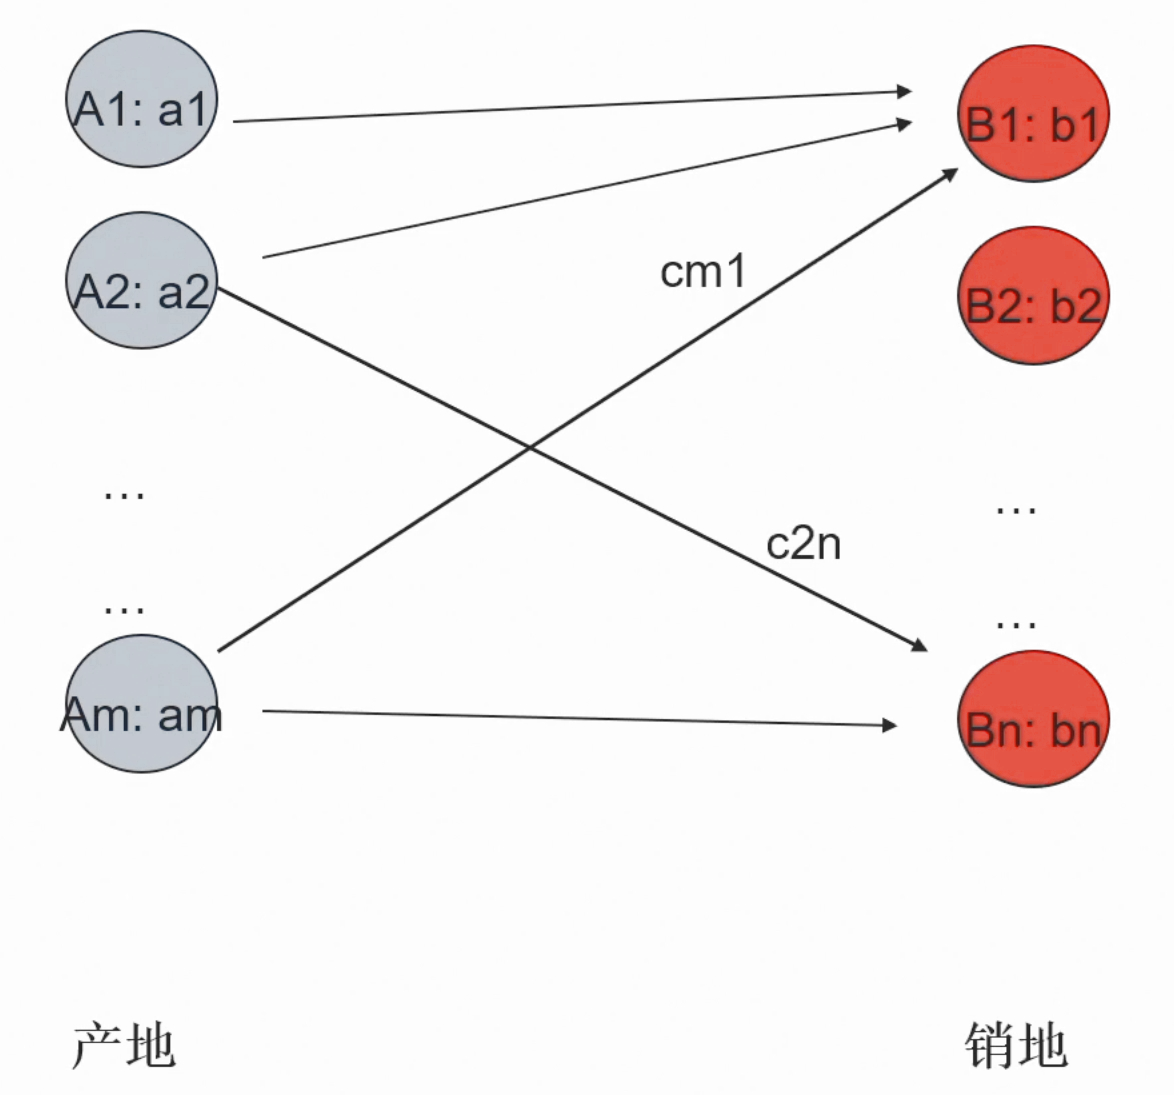
\includegraphics[width=0.6\textwidth]{./image/5.png}
    \caption{例1.1.3图解}
    \label{fig:Chapter3_Temporary_Pavilion_1}
\end{figure}
优化目标为最小化总运费,数学模型如下:

\begin{equation}
\min z = \sum_{i=1}^{m} \sum_{j=1}^{n} c_{ij} x_{ij}
\end{equation}

约束条件:
\begin{align}
&\sum_{j=1}^{n} x_{ij} = a_i, \quad i = 1, 2, \dots, m \tag{m 个约束方程} \\
&\sum_{i=1}^{m} x_{ij} = b_j, \quad j = 1, 2, \dots, n \tag{n 个约束方程} \\
&x_{ij} \geq 0, \quad i = 1, 2, \dots, m; \, j = 1, 2, \dots, n \tag{m $\times$ n 个变量}
\end{align}

约束条件的系数矩阵共 $m + n$ 行,$m \times n$ 列的矩阵,即 $x_{ij}$ 的系数向量。

\begin{equation}
\mathbf{p_{ij}} = (0, \dots, 1, \dots, 1, \dots, 0)^{\top}, \quad i \text{ 行, } m+j \text{ 行}
\end{equation}

分量中除第 $i$ 个和第 $m+j$ 个元素为 1,其余均为 0。
\\
关于产销平衡的运输问题,还有
\begin{equation}
\sum_{i=1}^{m} a_i = \sum_{i=1}^{m} \left( \sum_{j=1}^{n} x_{ij} \right) = \sum_{j=1}^{n} \left( \sum_{i=1}^{m} x_{ij} \right) = \sum_{j=1}^{n} b_j \,,
\end{equation}

所以模型中最多有 $m+n-1$ 个独立约束方程,即系数矩阵的秩不超过 $m+n-1$\footnote{原本有$m+n$个方程,但是根据题目中提到的“产销平衡”,可以列出方程3.3,即自由度减1,消去了一个约束,可行域增大}。
\end{exbox}

\subsection{产销不平衡}
事实上,我们知道,市场上几乎不可能出现“产销平衡”的情况,供大于求(产大于销)、供不应求(销大于产)的情况更为常见。
\textcolor{red}{产销不平衡问题一般都是转化为产销平衡问题解决的。}
\begin{exbox}{\textbf{产销不平衡的运输问题}}
    1
    \begin{enumerate}
        \item[(1)] \textbf{产大于销时:}
        
        由于
        \begin{equation}
            \sum_{j=1}^{n} b_j < \sum_{i=1}^{m} a_i \,,
        \end{equation}
        
        则问题的模型为
        \begin{equation}
            \min z = \sum_{i=1}^{m} \sum_{j=1}^{n} c_{ij} x_{ij} \,,
        \end{equation}
        
        约束条件:
        \begin{align}
            \sum_{j=1}^{n} x_{ij} &\leq a_i \quad i=1,2,\dots,m \,, \\
            \sum_{i=1}^{m} x_{ij} &= b_j \quad j=1,2,\dots,n \,, \\
            x_{ij} &\geq 0 \quad i=1,2,\dots,m;\ j=1,2,\dots,n \,.
        \end{align}
        其中,$\sum_{j=1}^{n} x_{ij} \leq a_i$ 表示 $i$ 产品的总产量小于或等于其产量。
        \\
        \item[(2)] \textbf{销大于产时:}
        
        由于
        \begin{equation}
            \sum_{j=1}^{n} b_j > \sum_{i=1}^{m} a_i \,,
        \end{equation}
        
        则问题的数学模型为
        \begin{equation}
            \min z = \sum_{i=1}^{m} \sum_{j=1}^{n} c_{ij} x_{ij} \,,
        \end{equation}
        
        约束条件:
        \begin{align}
            \sum_{j=1}^{n} x_{ij} &= a_i \quad i=1,2,\dots,m \,, \\
            \sum_{i=1}^{m} x_{ij} &\leq b_j \quad j=1,2,\dots,n \,, \\
            x_{ij} &\geq 0 \quad i=1,2,\dots,m;\ j=1,2,\dots,n \,.
        \end{align}
        其中,$\sum_{i=1}^{m} x_{ij} \leq b_j$ 表示 $i$ 产品的总产量小于或等于其销量。
    \end{enumerate}
    
    此时,要将各约束资源
    \begin{equation}
        \sum_{i=1}^{m} a_i - \sum_{j=1}^{n} b_j = b_{n+1} \,,
    \end{equation}
    
    在生产地或销地储存起来,即使没有一个虚拟的销售地,其运费为零,即设 $x_{i,n+1}$ 表示产地 $A_i$ 多年产(需要储存)的物资数量,运费为 $c_{i,n+1}=0$ $(i=1,2,\dots,m)$,其目标函数不变。于是问题的模型变为
    \begin{equation}
        \min z = \sum_{i=1}^{m} \sum_{j=1}^{n} c_{ij} x_{ij} \,,
    \end{equation}
    
    约束条件:
    \begin{align}
        \sum_{j=1}^{n} x_{ij} + x_{i,n+1} &= a_i \quad (i=1,2,\dots,m) \,, \label{eq:balance1} \\
        \sum_{i=1}^{m} x_{ij} &= b_j \quad (j=1,2,\dots,n) \,, \label{eq:balance2} \\
        \sum_{i=1}^{m} x_{i,n+1} &= \sum_{i=1}^{m} a_i - \sum_{j=1}^{n} b_j = b_{n+1} \,, \label{eq:balance3} \\
        x_{ij}, x_{i,n+1} &\geq 0 \quad (i=1,2,\dots,m;\ j=1,2,\dots,n) \,. \label{eq:Chapter3_nonneg_1}
    \end{align}
    公式 \eqref{eq:balance1} 表示转化为产销平衡问题。
\end{exbox}
\begin{figure}[H]
    \centering
    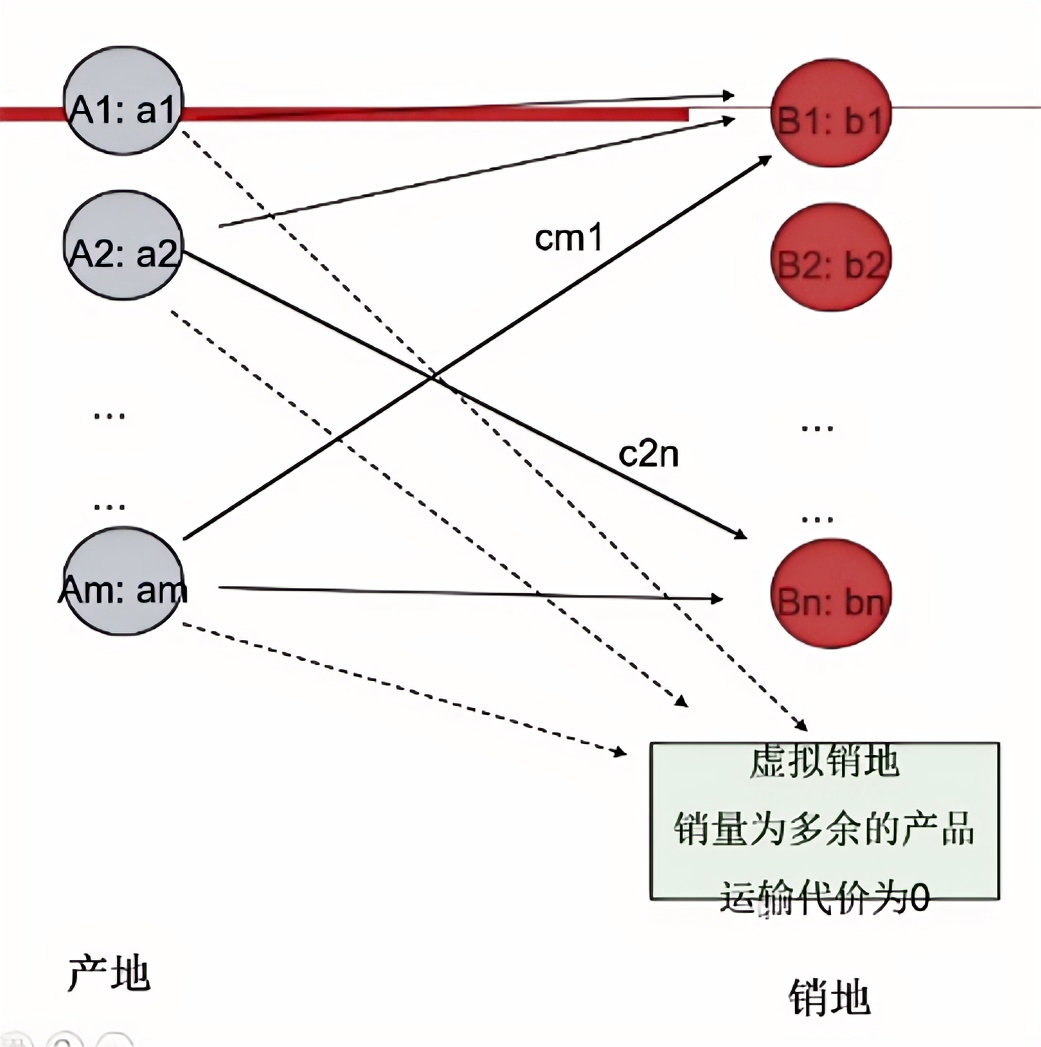
\includegraphics[width=0.5\textwidth]{./image/6.png}
    \caption{产大于销的情况}
    \label{fig:Chapter3_Temporary_Pavilion_2}
\end{figure}

\begin{figure}[H]
    \centering
    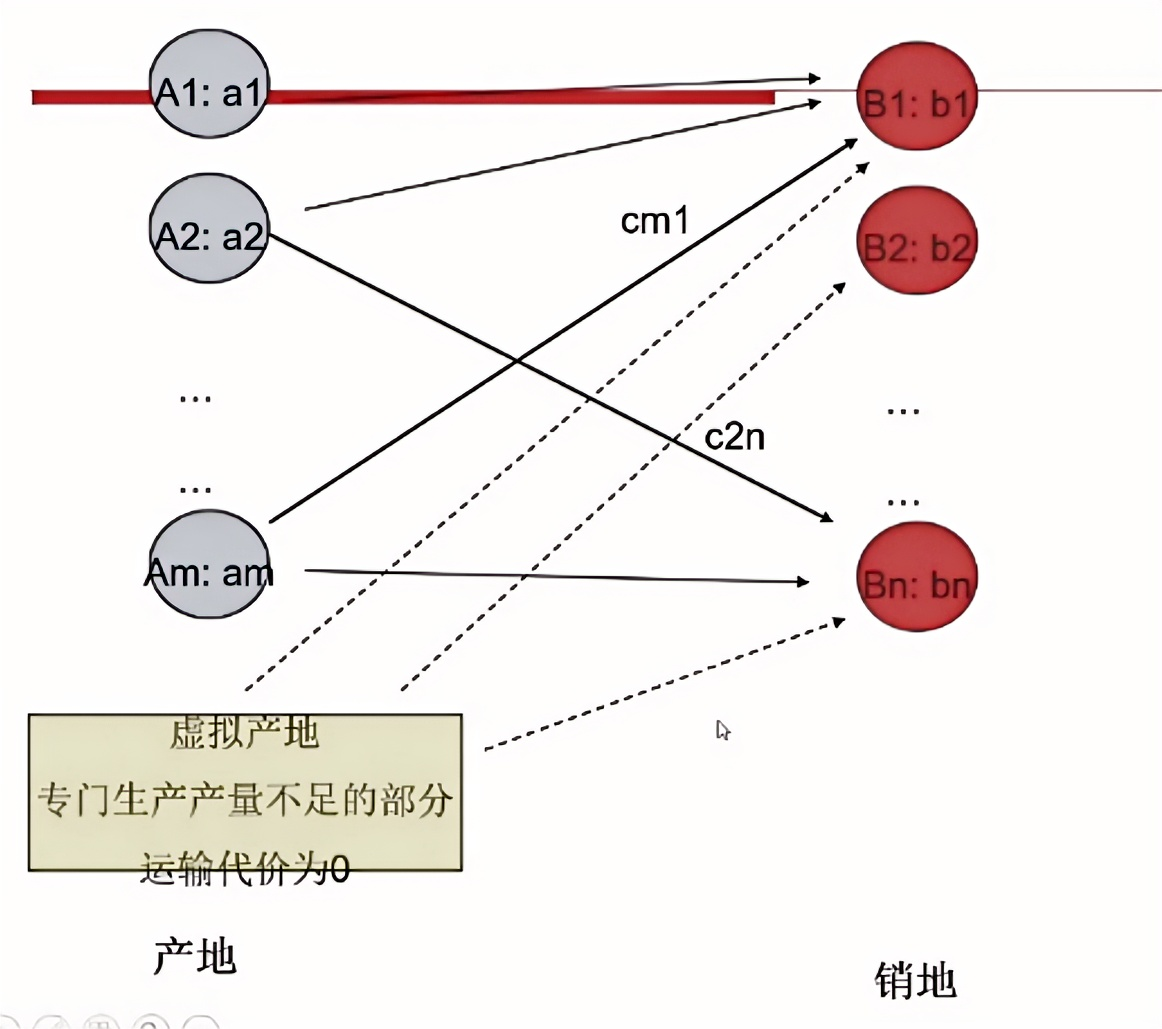
\includegraphics[width=0.5\textwidth]{./image/7.png}
    \caption{销大于产的情况}
    \label{fig:Chapter3_Temporary_Pavilion_3}
\end{figure}

\ifx\allfiles\undefined
	
	% 如果有这一部分的参考文献的话,在这里加上
	% 没有的话不需要
	% 因此各个部分的参考文献可以分开放置
	% 也可以统一放在主文件末尾。
	
	%  bibfile.bib是放置参考文献的文件,可以用zotero导出。
	% \bibliography{bibfile}
	
	end{document}
	\else
	\fi
    \ifx\allfiles\undefined

	% 如果有这一部分另外的package,在这里加上
	% 没有的话不需要
	
	\begin{document}
\else
\fi
    \chapter{整数规划}
    \section{整数规划问题与数学模型}
    \subsection{整数规划问题的定义}
    在前面的线性规划和运输规划问题中,最优解一般都是实数。但对于实际中的具体问题的解常常要求必须取整数,即称为整数解,
例如,问题答案是几个人、几台设备、几辆车等,无法用实数表达。因此,对于要求最优整数解的问题,就涉及到整数规划。
\begin{dfnbox}{整数规划}{amznotes}
    如果一个数学规划的\textcolor{red}{某些决策变量或全部决策变量}要求必须取\textcolor{red}{整数},则这样的问题称为\textbf{整数规划问题};
相应的模型称为\textbf{整数规划模型}。
\end{dfnbox}
\begin{itemize}
    \item \textbf{纯整数规划问题}:所有的决策变量都为\textcolor{red}{整数}的整数规划;
    \item \textbf{混合整数规划问题}:存在决策变量为\textcolor{red}{整数}的整数规划;
    \item \textbf{0-1规划}:所有的决策变量只能取\textcolor{red}{0或1}的整数规划;
\end{itemize}

\subsection{整数规划问题的数学模型}

\begin{thmbox}{一般形式的整数线性规划问题}{cool}
    \[
    \max(\min) \ z = \sum_{j=1}^{n} c_j x_j
    \]
    s.t.
    \[
    \begin{cases}
        \sum_{j=1}^{n} a_{ij} x_j \leq (\geq, =) b_i \,, & (i=1,2,\dots,m) \,, \\
        x_j \geq 0 \,, \quad x_j \text{ 为整数} & (j=1,2,\dots,n) \,.
    \end{cases}
    \]
\end{thmbox}

\begin{exbox}{\textbf{产品生产(纯整数规划问题)}}
    1\textbf{例}:某厂生产 $A_1$ 和 $A_2$ 两种产品,需要经过 $B_1$、$B_2$、$B_3$ 三道工序加工。单件工时和利润值以及各工序每月工时定额表 4.1。问工厂应如何安排生产才能使总利润最大?
    
    \begin{table}[H]
        \centering
        \label{tab:4.1}
        \renewcommand{\arraystretch}{1.5}
        \begin{tabular}{|c|c|c|c|c|}
            \hline
            & $B_1$ & $B_2$ & $B_3$ & 利润(元/件) \\ \hline
            $A_1$ & 0.3 & 0.2 & 0.3 & 25 \\ \hline
            $A_2$ & 0.7 & 0.1 & 0.5 & 40 \\ \hline
            工时定额(小时/月) & 250 & 100 & 150 & \\ \hline
        \end{tabular}
        \caption{工厂加工条件与利润}
    \end{table}
    
    \textbf{解:} 根据表 2-1 的最后一栏的利润数据,生产 $A_1$ 件、$A_2$ 件能获取的总利润为 $25x_1 + 40x_2$,因此,该问题的数学模型为:
    \begin{equation}
        \max \quad 25x_1 + 40x_2 \label{eq:Chapter4_obj_1}
    \end{equation}
    约束条件:
    \begin{align}
        0.3x_1 + 0.7x_2 &\leq 250 \,, \label{eq:c1} \\
        0.2x_1 + 0.1x_2 &\leq 100 \,, \label{eq:c2} \\
        0.2x_1 + 0.5x_2 &\leq 150 \,, \label{eq:c3} \\
        x_1 \geq 0 \,, \quad x_2 &\geq 0 \,. \label{eq:Chapter4_nonneg_1}
    \end{align}
    这是一个纯整数规划问题。
    
    \textbf{解}:设工厂每月生产 $A_1$ 产品 $x_1$ 件,$A_2$ 产品 $x_2$ 件。则按表 2-1 提供的条件数据,$A_1$ 产品 $x_1$ 件、$A_2$ 产品 $x_2$ 件加工需要的总利润为 $25x_1 + 40x_2$,因此,该问题的数学模型为:
    \begin{equation}
        \max \quad 25x_1 + 40x_2
    \end{equation}
    约束条件:
    \begin{align}
        0.3x_1 + 0.7x_2 &\leq 250 \,, \tag{$B_1$ 工序,工时限制} \\
        0.2x_1 + 0.1x_2 &\leq 100 \,, \tag{$B_2$ 工序,工时限制} \\
        0.2x_1 + 0.5x_2 &\leq 150 \,, \tag{$B_3$ 工序,工时限制} \\
        x_1 \geq 0 \,, \quad x_2 &\geq 0 \,. \tag{且只能整数}
    \end{align}
    另外,由于 $x_1$ 为 $A_1$ 的件数,因此 $x_1 \geq 0$ 且只能取整数;同理,$x_2 \geq 0$ 且只能取整数。
\end{exbox}


\begin{exbox}{\textbf{背包问题(0-1规划)}}
    1\textbf{例}:一个背包的总容积为 $V$,现要在 $n$ 种物品中选择。设物品 $j$ 的重量为 $w_j$,体积为 $v_j$,$j=1,2,\dots,n$。问如何选择,使得到的总价值最大,且总重量不超过 $V$,又使装的总重量最大。这一个题目有 $n$ 个约束情况,如装某类装箱,装箱,装车等。
    
    \textbf{解:} 设对于物品 $j$,变量
    \[
    x_j = \begin{cases} 
        1 & \text{物品 $j$ 被装入背包} \\ 
        0 & \text{物品 $j$ 不被装入背包}
    \end{cases} \quad j=1,2,\dots,n
    \]
    则所有被选择装物品的总体积为 $\sum_{j=1}^{n} v_j x_j$,总重量为 $\sum_{j=1}^{n} w_j x_j$,该问题的数学模型为:
    \begin{equation}
        \max \sum_{j=1}^{n} w_j x_j \label{eq:Chapter4_obj_2}
    \end{equation}
    约束条件:
    \begin{align}
        \sum_{j=1}^{n}  &v_j x_j\leq V \,, \label{eq:constraint} \\
        x_j &= 0, 1 \,, \quad j=1,2,\dots,n \,. \label{eq:binary}
    \end{align}
    这是一个 0-1 规划问题。
\end{exbox}


    \section{一般整数规划的求解方法—分枝定界法}
    为了解决整数规划问题,我们自然想到两种办法:
    \begin{itemize}
        \item 想到第二章提到的下料问题,可以用线性规划求解,结果四舍五入;
        \item 反正是整数,不妨穷举求解;
    \end{itemize}
    显然第一个方法不够靠谱,第二个方法效率太低。\\
    \begin{exbox}{\textbf{第一个方法不靠谱的原因}}
    1例如, 考虑如下整数规划问题:
    \begin{align}
        \max \ 3x_{1} &+ 13x_{2} \\
        \text{s.t.} \quad 2x_{1} + 9x_{2} &\leq 40 \\
        11x_{1} - 8x_{2} &\leq 82 \\
        x_{1} \geq 0, \quad x_{2} &\geq 0 \quad \text{且取整数}
    \end{align}
    画出可行域如下所示\footnote{图中可以看到,浮点数最优解 B四周的四个整数点都不在可行域内,四舍五入的结果是错误的。反而整数最优解在C点。}:
    \begin{figure}[H]
        \centering
        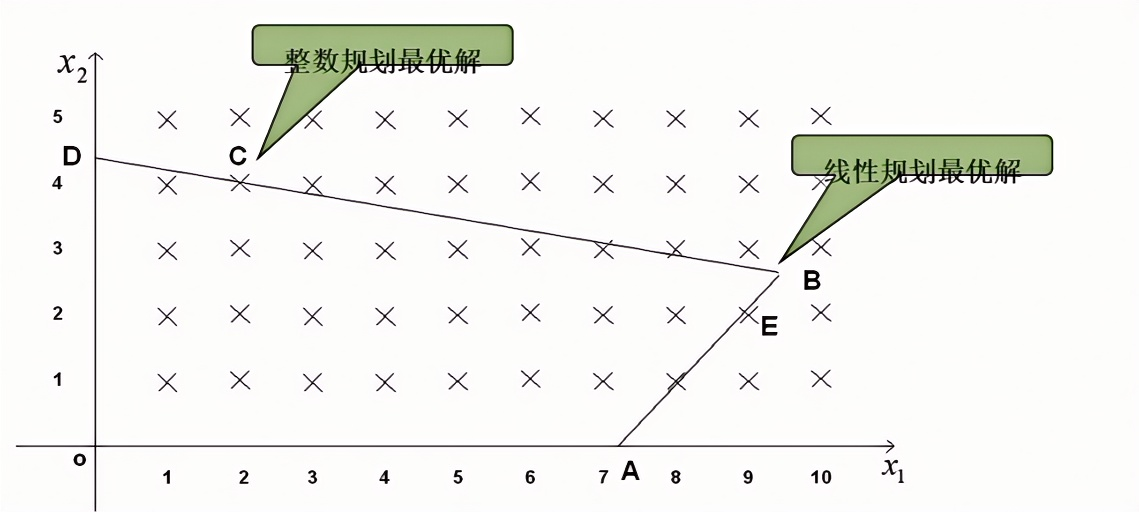
\includegraphics[width=0.8\textwidth]{./image/8.png}
        \caption{整数规划的四舍五入求解}
        \label{fig:Chapter4_Temporary_Pavilion_1}
    \end{figure}
    \end{exbox}

    目前,常用的求解整数规划的方法是分枝定界法和割平面法。作为一种最基本的方法,下面介绍分枝定界法。
    \begin{notebox}{\textbf{分枝定界法}}
        \label{分枝定界法}
        \\
        \begin{enumerate}
            \item 设有最大化的整数规划问题A,与它相应的线性规划问题(即在整数规划中去掉了决策变量的整数取值要求)为B,设二者的最优值分别为$z_A^*$和$z_B^*$;
            \item 从解问题B开始,若B的最优解符合A中的整数条件,\textcolor{red}{则A的最优解即为B的最优解},结束;
            \item 若B的最优解不符合A的整数条件,则B的最优解对应的最优值$z_B^*$一定是\textcolor{red}{A的最优值$z_A^*$的上界},记为$\overline{z}$ ,而A的某一\textcolor{red}{任一可行解}(即任意一个整数解)的目标函数值将是一个下界$\underline{z}$。此时$\underline{z}\leq z_A^* \leq \overline{z}$,称为\textbf{定界};
            \item 分枝定界法即不断将B的可行域分成子区域(称为\textbf{分枝}),并在每个子区域中确定A的\textcolor{red}{上界$\overline{z}$和下界$\underline{z}$}的方法,逐步夹逼,直到找到A的最优解为止;
        \end{enumerate}
    \end{notebox}

    \begin{figure}[H]
        \centering
        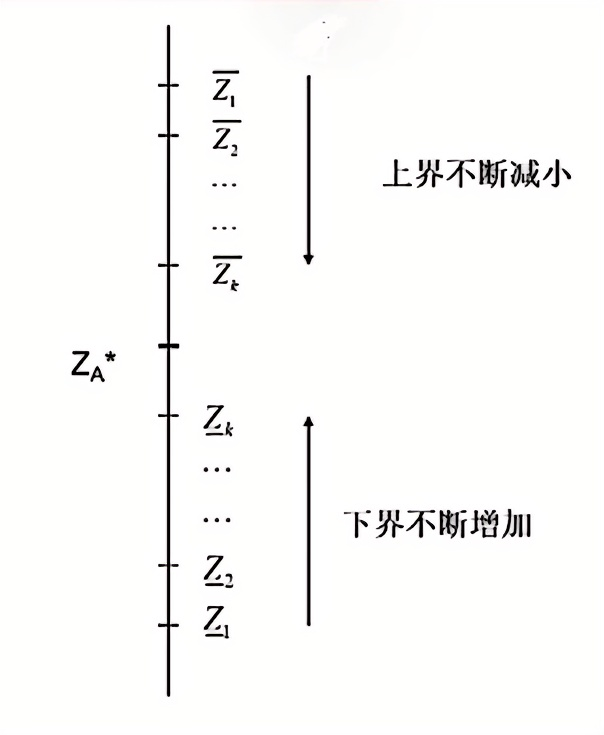
\includegraphics[width=0.5\textwidth]{./image/9.png}
        \caption{分枝定界法}
        \label{fig:Chapter4_Temporary_Pavilion_2}
    \end{figure}
    \begin{exbox}{\textbf{分枝定界法}}
        1\textbf{例:}\ 考虑如下整数规划问题:
        \begin{align}
            \max \ 40x_{1} &+ 90x_{2} \\
            \text{s.t.} \quad 9x_{1} + 7x_{2} &\leq 56 \\
            7x_{1} + 20x_{2} &\leq 70 \\
            x_{1} \geq 0, \quad x_{2} &\geq 0 \quad \text{且取整数}
        \end{align}
        \textbf{解:}\ 记上述原问题为A。先考虑A中去掉整数约束条件后的线性规划问题B.
        \\
        对问题B进行第二章中所学到的线性规划分析,可以找到最优解,依照\hyperref[分枝定界法]{分枝定界法},发现B的最优解并非整数,说明\textcolor{red}{需要继续迭代},因此我们记B的最优解对应的最优值$z_B^*=356$作为一个上界,并任意找一个A的可行解如原点,得到下限$\underline{z}=0$,此时$\underline{z}\leq z_A^* \leq \overline{z}$,即$0\leq z_A^* \leq 356$。如下图所示:\\
        \begin{figure}[H]
            \centering
            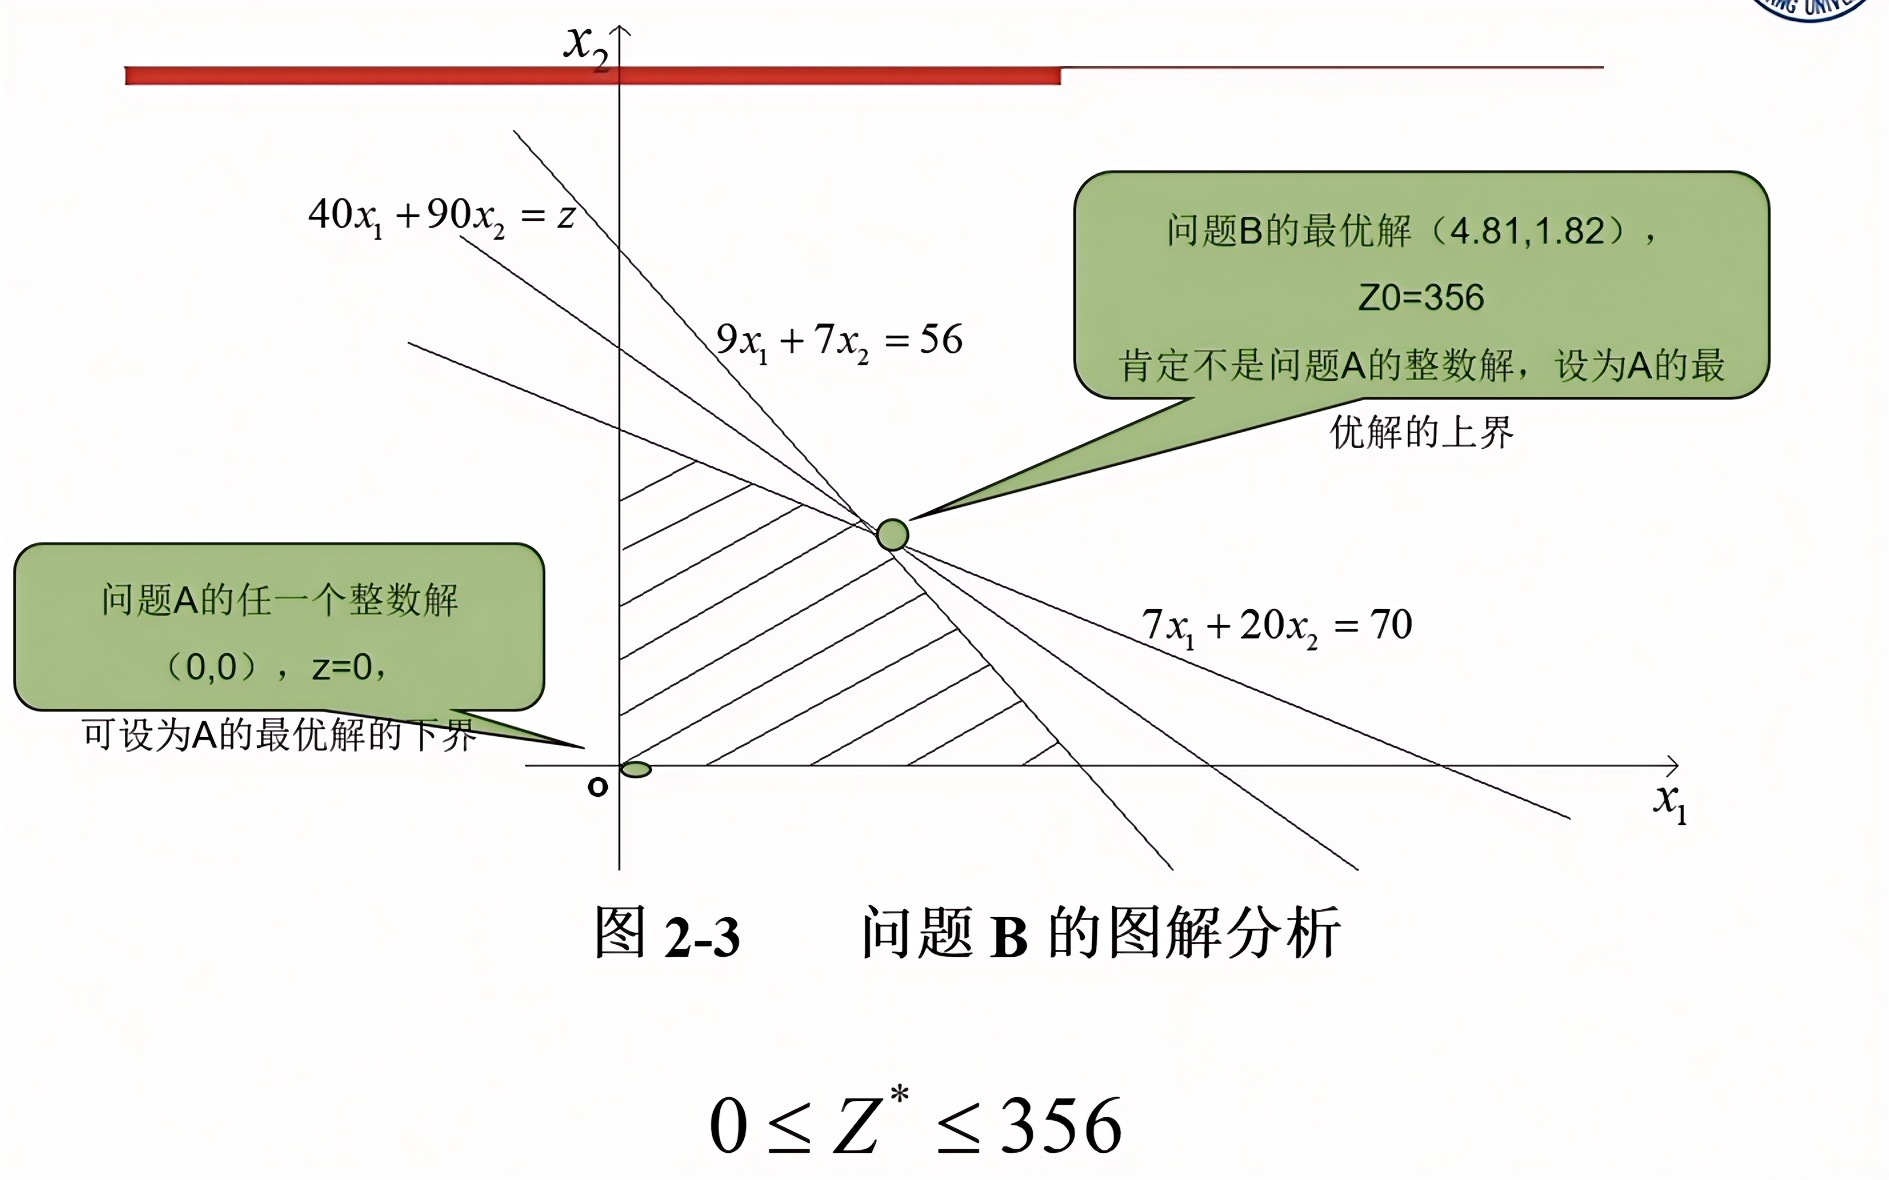
\includegraphics[width=0.8\textwidth]{./image/11.png}
            \caption{问题B的图解分析}
            \label{fig:Chapter4_Temporary_Pavilion_3}
        \end{figure}
        在问题 B 中最优解为 \( {x}_{1} = {4.81} \) ,于是对 B 通过增加两个
        约束条件 \( {x}_{1} \leq  4 \) 和 \( {x}_{1} \geq  5 \) 可将 B 分解为两个子问题 \( {B}_{1} \) 和 \( {B}_{2} \) ,即将 B
        的可行域在 \( {x}_{1} = {4.81} \) 前后分割为两个子可行域(称为分枝), 中间因为不满足整数条件而舍弃,如下图所示:
        \begin{figure}[H]
            \centering
            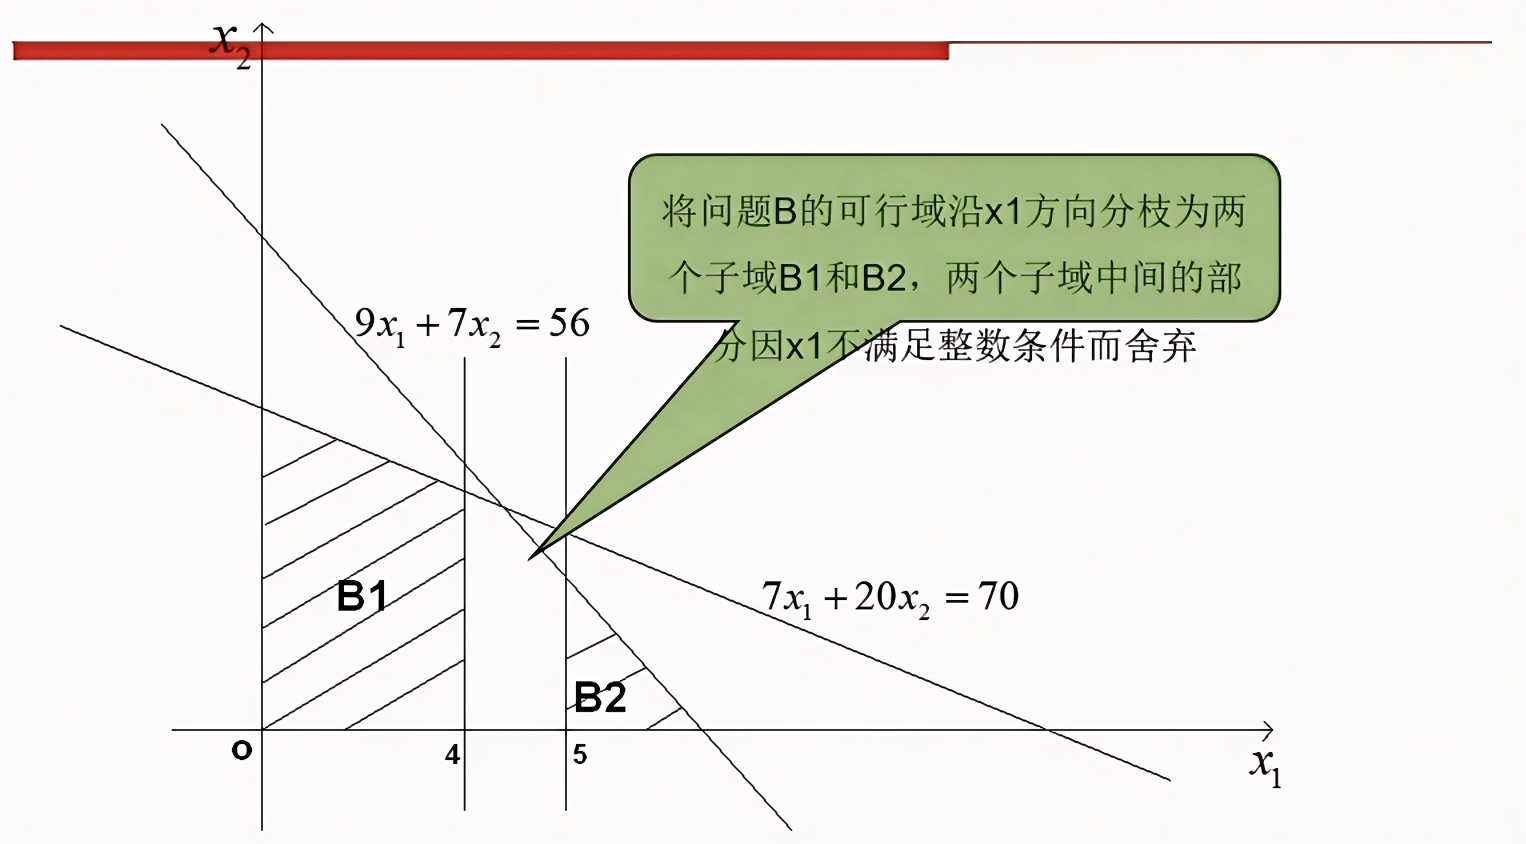
\includegraphics[width=0.8\textwidth]{./image/10.png}
            \caption{问题B的分枝}
            \label{fig:Chapter4_Temporary_Pavilion_4}
        \end{figure}
        对应的 $\text{B}_1$ 和 $\text{B}_2$ 分别为:

        \textbf{问题 B1}:
        
        \begin{align*}
        \max \quad & 40x_1 + 90x_2 \\
        \text{s.t.} \quad & 9x_1 + 7x_2 \leq 56 \\
        & 7x_1 + 20x_2 \leq 70 \\
        & 0 \leq x_1 \leq 4 \\
        & x_2 \geq 0
        \end{align*}
        
        \textbf{问题 B2}:
        
        \begin{align*}
        \max \quad & 40x_1 + 90x_2 \\
        \text{s.t.} \quad & 9x_1 + 7x_2 \leq 56 \\
        & 7x_1 + 20x_2 \leq 70 \\
        & x_1 \leq 5 \\
        & x_2 \geq 0
        \end{align*}
        \textbf{这样,我们进行第一次迭代。}\\
        在两个区域内分别线性规划求解,如下图所示,两处最优解仍然不都是整数,说明\textcolor{red}{需要继续迭代}。B1区域的最优值是$z_{B1}^* = 349$,B2区域的最优值是$z_{B2}^* = 341$,取较大的那个,因此新的上限是$z_{B1}^* = 349$,下限依然是$z_{B}^* = 0$(注意下界此处不是不可以动,而是我们懒得去动),所以我们将上限从原来的356调整为349,此时$0\leq z_A^* \leq 349$。\\
        \begin{figure}[H]
            \centering
            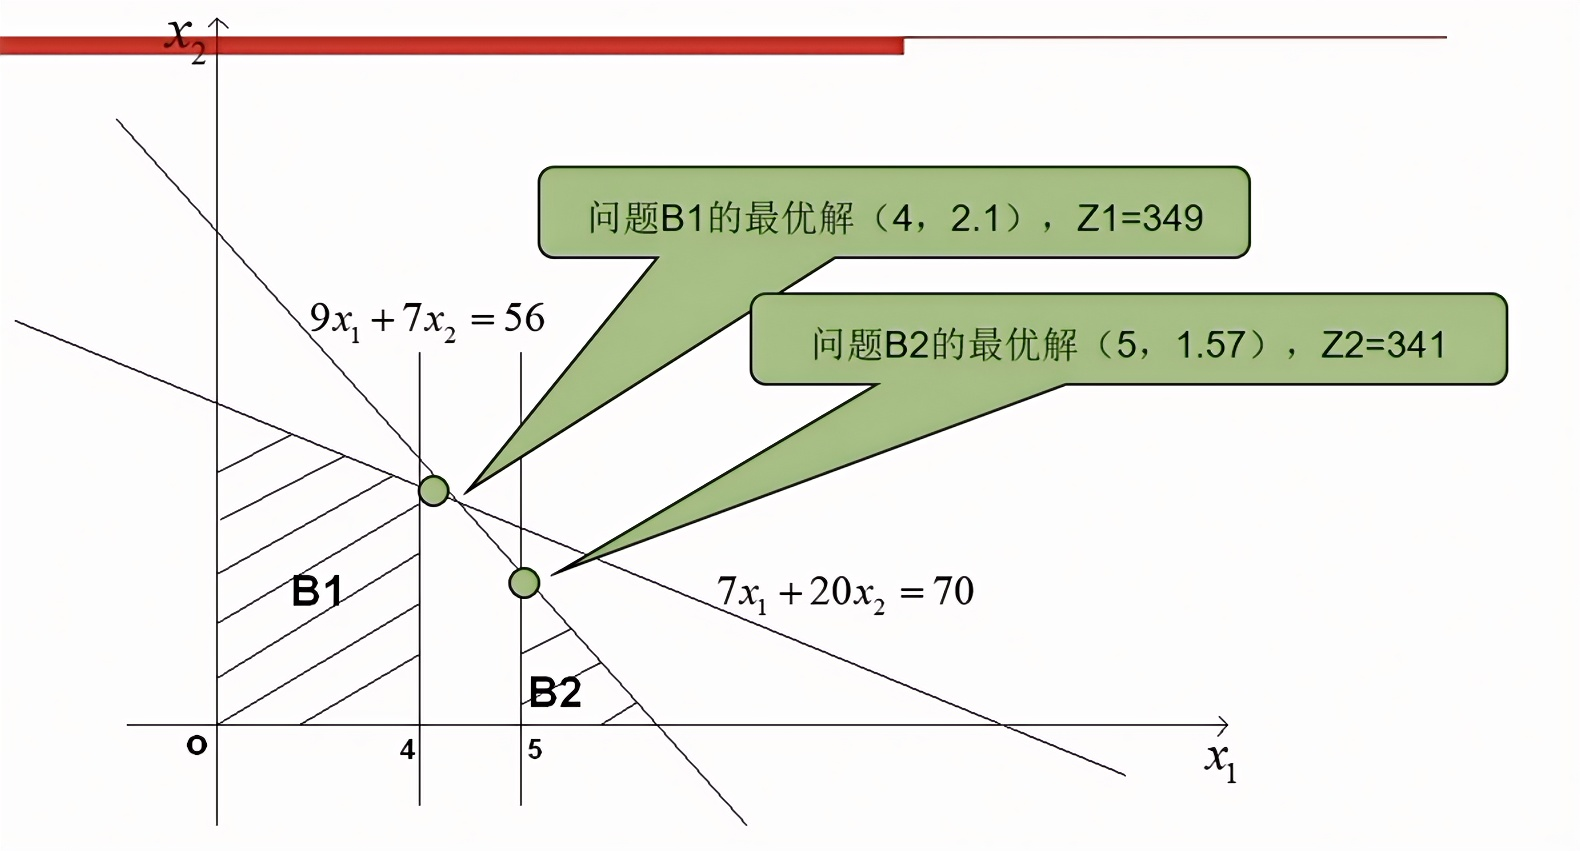
\includegraphics[width=0.8\textwidth]{./image/12.png}
            \caption{第一次迭代}
            \label{fig:Chapter4_Temporary_Pavilion_4}
        \end{figure}
        继续对 \( \text{B}_{1} \) 和 \( \text{B}_{2} \) 进行分解。因 \( {z}_{1} > {z}_{2} \) ,故先分解 \( \text{B}_{1} \) 为两枝。此
        次沿 \( {x}_{2} \) 方向分解,增加约束条件 \( {x}_{2} \leq  2 \) ,称为问题 \( \text{B}_{3} \) ; 增加约束
        条件 \( {x}_{2} \geq  3 \) ,称为问题 \( \text{B}_{4} \) 。在图 2-4 中舍去 \( {x}_{2} > 2 \) 与 \( {x}_{2} < 3 \) 之间的
        可行域。\\
        \textbf{这样,我们进行第二次迭代。}\\
        在两个区域内分别线性规划求解,可以发现B3的最优点仍是顶点,恰好是整数$(4,2)$\footnote{读者不妨想到此事并非偶然。事实上,由于我们的切割线总是$x_1=a$或$x_2=b$,总是能割出一个区域为矩形,顶点就是整数解},最优值是$z_{B3}^* = 340$,
        这个数可能是上界(即整数里最优的),也可能不是,但至少一定是整数中的一员,所以肯定可以作为下界\footnote{读者可能会感到疑问,之前方法里不是说算到是整数解就应该停止迭代作为最优解了吗?为什么还要继续算呢?读者不妨想到,这个整数解确实是最优解,但是不是问题A的最优解,而是问题B3对应的A3的最优解,所以仍需要证明其他区域内没有比这个更大或者有更大的最优值了}。而B4的最优值都比不上我们新的下界了,那B4就失去了意义,不必再分割了;同理B3也不需要再分割了,最大值是下限,再求B3也没有比340更大的整数解了;但是B2有必要继续去做切割。如下图所示:
        \begin{figure}[H]
            \centering
            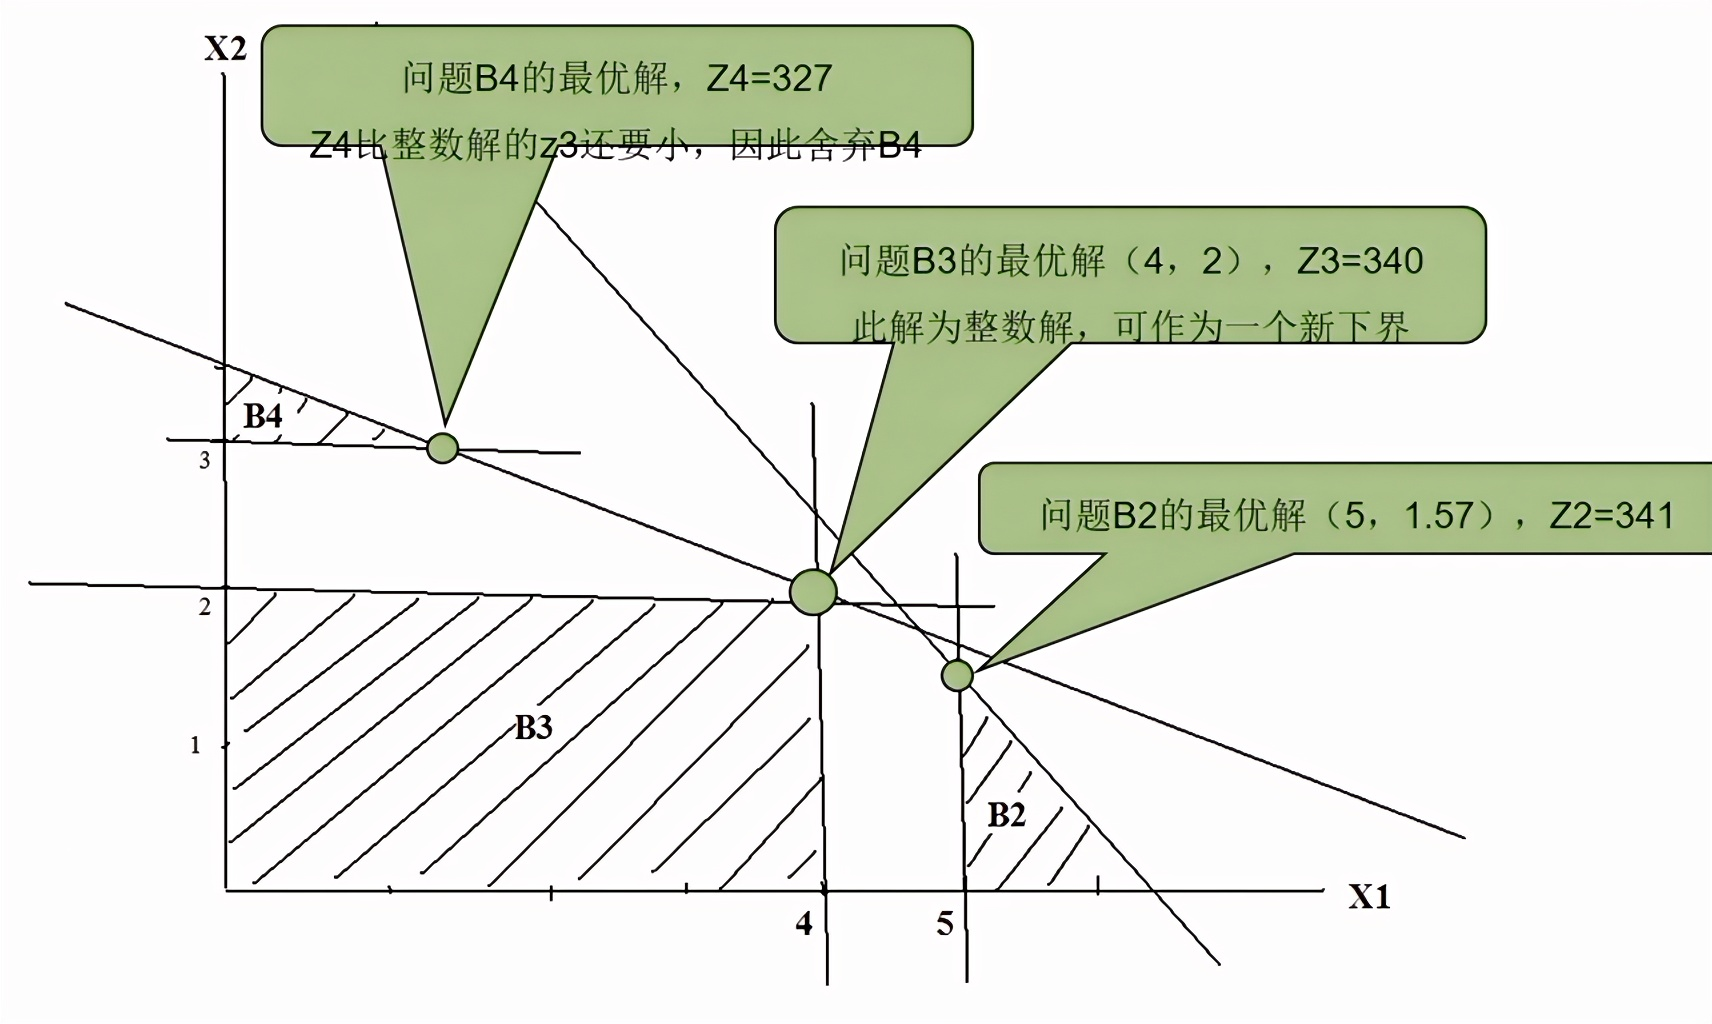
\includegraphics[width=0.8\textwidth]{./image/13.png}
            \caption{第二次迭代}
            \label{fig:Chapter4_Temporary_Pavilion_4}
        \end{figure}
        既然 $\text{B}_1$ 中已不存在上限,于是分解 $\text{B}_2$ 得以下问题:\\
        \textbf{问题 B5}:
        \begin{align*}
        \max \quad & 40x_1 + 90x_2 \\
        \text{s.t.} \quad & 9x_1 + 7x_2 \leq 56 \\
        & 7x_1 + 20x_2 \leq 70 \\
        & 5 \leq x_1 \\
        & 0 \leq x_2 \leq 1
        \end{align*}
        \textbf{问题 B6}:
        \begin{align*}
        \max \quad & 40x_1 + 90x_2 \\
        \text{s.t.} \quad & 9x_1 + 7x_2 \leq 56 \\
        & 7x_1 + 20x_2 \leq 70 \\
        & 5 \leq x_1 \\
        & 2 \leq x_2
        \end{align*}
        \textbf{这样,我们进行第三次迭代。}\\
        在两个区域内分别线性规划求解,可以发现B6没有可行解,故B6不再需要分割;B5的最优解$z_{B5}^* = 308$小于下限,故B5不再需要分割;因此,可以得出结论,最优解就是$z_{B3}^* = 340$如下图所示:
        \begin{figure}[H]
            \centering
            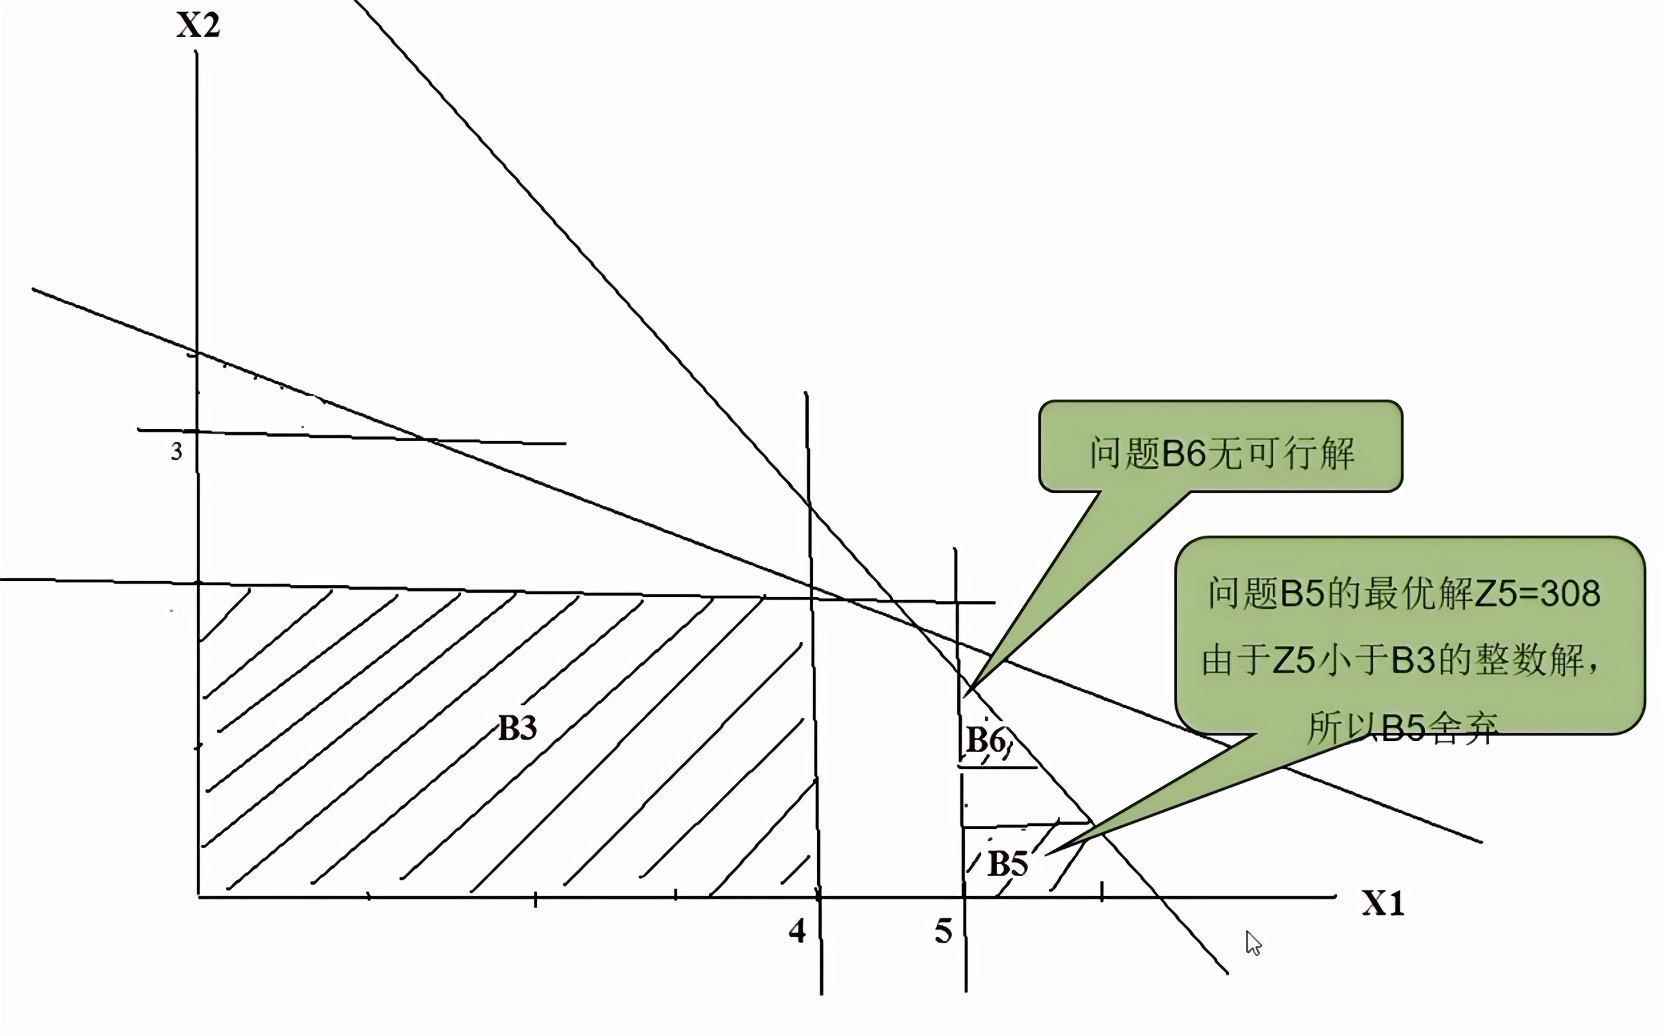
\includegraphics[width=0.8\textwidth]{./image/14.png}
            \caption{第三次迭代}
            \label{fig:Chapter4_Temporary_Pavilion_4}
        \end{figure}

        \end{exbox}
        我们不难发现,在上述过程中,除了最开始找了任意一个整数点作为下限,
        其他的计算过程全部是\textcolor{red}{线性规划}的过程。即过程分为两类:
        \begin{itemize}
            \item (计算过程)线性规划求解:即求解B问题的最优解。
            \item (判断过程)分枝:即对B问题进行分割,得到子区域B1、B2、B3、B4等。同时进行判断并更新上限和下限。
        \end{itemize}
        实际上我们在做的,就是先算B问题的最优解,如果需要则进行分割,再分别算子区域的最优解。并依据子区域更新上限和下限。实际上是取各个子区域上下限的交集。
        \begin{itemize}
            \item 如果发现子区域最优值小于等于当前下限,则该子区域没有继续分割的必要了。
            \item 如果发现子区域最优值小于当前上限,则应该更新上限。
            \item 如果上下限互相逼近到相等,问题可以结束。即证明某一子区域整数最优解所对应的最优值比其他子区域的都要大。
        \end{itemize}
        \begin{notebox}{\textbf{分枝定界法的要点}}
            \begin{itemize}
                \item \textbf{分枝}:分为多个更小的空间
                \item \textbf{定界}:确定每个小空间的上、下限和总的上、下界
                \item \textbf{剪枝}:据每个小空间的上、下限和总的上、下界,删掉那些明显\textcolor{red}{低于总下界}和\textcolor{red}{无可行解}的小空间。
            \end{itemize}
        \end{notebox}
        \begin{figure}[H]
            \centering
            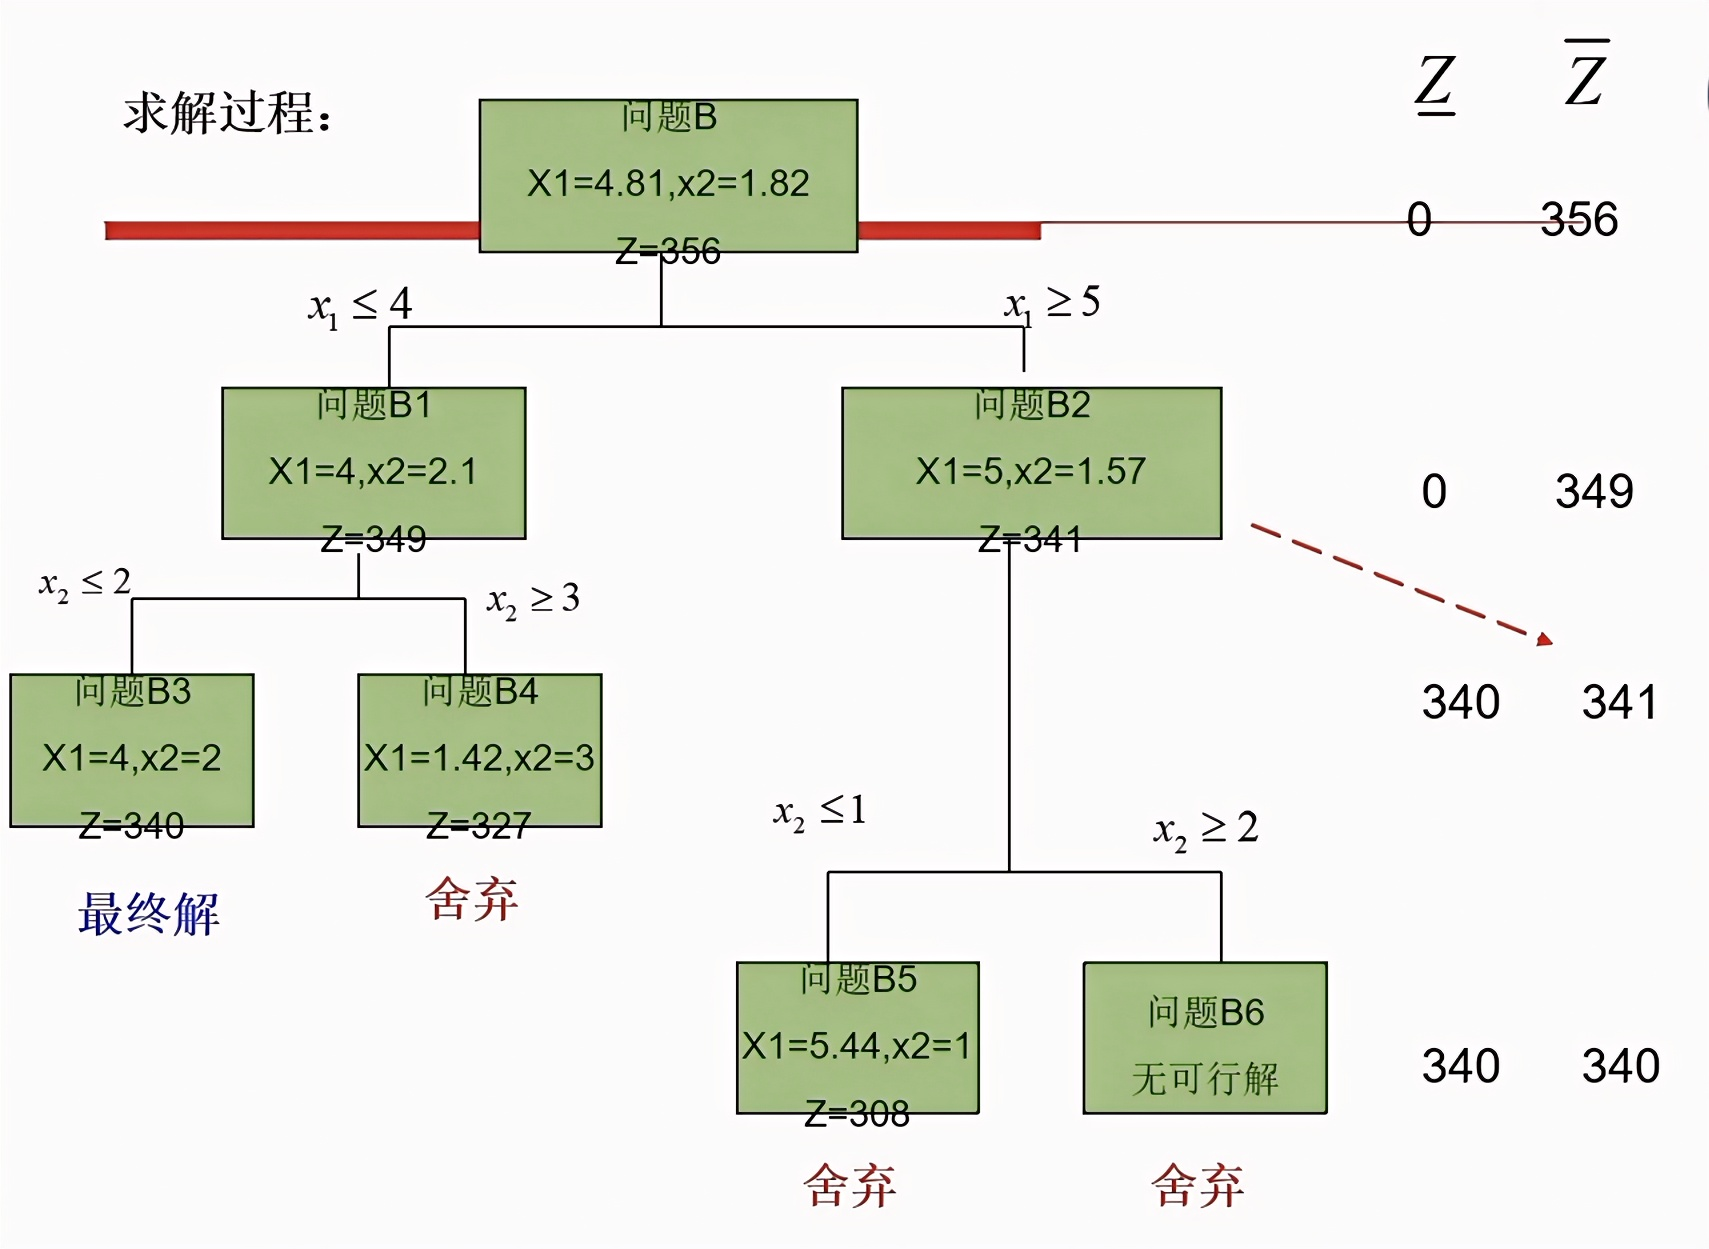
\includegraphics[width=0.8\textwidth]{./image/15.png}
            \caption{例题总体思路}
            \label{fig:Chapter4_Temporary_Pavilion_4}
        \end{figure}
    
    \section{0-1规划及其求解方法}
    \subsection{0-1规划的定义和数学模型}
    \begin{dfnbox}{0-1规划}{amznotes}
        如果整数规划问题中的所有决策变量 $x_i$,$(i=1, 2, \cdots, n)$ 仅限于取 0 或 1 两个值,则称此问题为 0-1 整数规划,简称为\textbf{0-1 规划},其变量 $x_i$,$(i=1, 2, \cdots, n)$ 称为\textbf{0-1 变量},或\textbf{二进制变量},相应的决策变量取值的约束为 $x_i = 0$ 或 1,等价于 $x_i \geq 0$ 且 $x_i \leq 1$,且为整数。
    \end{dfnbox}
    \begin{dfnbox}{0-1混合整数规划}{amznotes}
        如果整数规划问题中的一部分决策变量为 0-1 变量,则称为 \textbf{0-1 混合整数规划}。
    \end{dfnbox}
    0-1 规划可以是线性的,也可以是非线性的,0-1 整数规划的一般模型为:
    \begin{thmbox}{0-1 整数规划的一般模型}{cool}
        \begin{center}
            \begin{equation*}
            \max \quad (\min) \quad z = \sum_{j=1}^n c_j x_j
            \end{equation*}
            \begin{equation*}
            \text{s.t.} \quad \sum_{j=1}^n a_{ij} x_j \leq (\text{或 } =, \geq) \, b_i \quad (i=1, 2, \cdots, m),
            \end{equation*}
            \begin{equation*}
            x_j = 0 \text{ 或 } 1 \quad (j=1, 2, \cdots, n).
            \end{equation*}
            \end{center}
    \end{thmbox}

    \subsection{0-1规划的例题}
    \begin{exbox}{\textbf{销售网点问题}}
    1\textbf{例:} 某公司拟在城东、城西、城南新建销售网点,有 7 个位置 A1, A2, A3, A4, A5, A6, A7 可选。考虑组建成本和总体布局,规定:

    \textbf{城东:} A1, A2, A3 中至多选择 2 个

    \textbf{城西:} A4, A5 中至少选择 1 个

    \textbf{城南:} A6, A7 至少选择 1 个

    若选 $A_i$,则建设投资为 $b_i$,预计获利 $c_i$,但投资总额不能超过 $B$ 元。如何选择址获利最大?
    \\
    \textbf{解:} 设决策变量 $x_i(i=1,2\cdots 7)$

    \begin{center}
    \begin{equation*}
    x_i = 
    \begin{cases} 
    1 & \text{A}_i \text{被选中}, \quad i=1,2\cdots 7 \\
    0 & \text{A}_i \text{未选中}
    \end{cases}
    \end{equation*}
    \end{center}

    则

    \begin{align*}
    \max \quad z &= \sum_{i=1}^7 c_i x_i \\
    \text{s.t.} \quad & \sum_{i=1}^7 b_i x_i \leq B \\
    & x_1 + x_2 + x_3 \geq 2 \\
    & x_4 + x_5 \geq 1 \\
    & x_6 + x_7 \geq 1 \\
    & x_i = 0,1, \quad i=1,2\cdots 7
    \end{align*}

    为 0-1 规划。
    \end{exbox}

    \begin{exbox}{\textbf{一般的指派问题(分派问题)}}
        1\textbf{例:} 在实际生产管理中,总希望把有限的资源(人员、资金等)最佳地指派,以发挥其最高的工作效率,创造最大的价值。
        例如,某科研部门有n项任务,正好需要n个人去完成,由于任务的性质和每个人的专长不同,每个人完成各项任务的效率(时间或成本)如表4.2所示。如果指派每个人仅能完成一项任务,每项任务仅要一个人去完成,如何分派使完成这n项任务的总效率(效益量化)为最高,这是典型的标准指派问题。
        \begin{table}[H]
            \centering
            \label{tab:4-2}
            \renewcommand{\arraystretch}{1.5}
            \begin{tabular}{|c|c|c|c|c|}
                \hline
                人$\backslash$项 & 1 & 2 & $\cdots$ & n \\
                \hline
                1 & $c_{11}$ & $c_{12}$ & $\cdots$ & $c_{1n}$ \\
                \hline
                2 & $c_{21}$ & $c_{22}$ & $\cdots$ & $c_{2n}$ \\
                \hline
                $\vdots$ & $\vdots$ & $\vdots$ & $\ddots$ & $\vdots$ \\
                \hline
                n & $c_{n1}$ & $c_{n2}$ & $\cdots$ & $c_{nn}$ \\
                \hline
            \end{tabular}
            \caption{指派问题的利润元成表矩阵}
        \end{table}
        
        \textbf{解:} 设指派问题的效益矩阵为 $(c_{ij})_{n \times n}$,其元素 $c_{ij}$ 表示指派第 $i$ 个人去完成第 $j$ 项任务时所获得的效益($>0$)。或者说:以 $c_{ij}$ 表示指派给 $i$ 的第 $j$ 单位资源分配用于第 $j$ 项任务时的有关效益。设问题的决策变量为 $x_{ij}$,是 0-1 变量,即
        
        \begin{center}
        \begin{equation*}
        x_{ij} = 
        \begin{cases} 
        1, & \text{当指派第 $i$ 个人去完成第 $j$ 项任务时}, \\
        0, & \text{当下指派第 $i$ 个人去完成第 $j$ 项任务时}.
        \end{cases}
        \end{equation*}
        \end{center}
        
        则其数学模型为
        
        \begin{align*}
        &\max (\min) \quad z = \sum_{i=1}^n \sum_{j=1}^n c_{ij} x_{ij} \\
        \text{s.t.} \quad & \sum_{j=1}^n x_{ij} = 1 \quad (i=1, 2, \cdots, n), \tag*{第 $i$ 个人做成一项任务} \\
        & \sum_{i=1}^n x_{ij} = 1 \quad (j=1, 2, \cdots, n), \tag*{第 $j$ 项任务只能由一个人完成} \\
        & x_{ij} = 0 \text{ 或 } 1 \quad (i, j=1, 2, \cdots, n).
        \end{align*}
        \end{exbox}

    \subsection{0-1规划的求解}
    \begin{dfnbox}{显枚举法}{amznotes}
        显枚举法(又称为穷举法)是把所有可能的组合情况(共2n种组合)列举出后进行比较,找到所需要的解。这种方法对于变量个数较多时,易产生“组合爆炸”,计算量非常巨大。
    \end{dfnbox}
    \begin{dfnbox}{隐枚举法}{amznotes}
        隐枚举法是从实际出发,从所有可能的组合取值中利用过滤条件排除些不可能是最优解的情况,只需考查一部分的组合就可以得到最优解。因此,隐枚举法又称为部分枚举法。
    \end{dfnbox}
    \begin{exbox}{隐枚举求解}
        1\textbf{例:} 用隐枚举求解
        \[
        \max \quad z = 3x_1 - 2x_2 + 5x_3
        \]

        \[
        \begin{array}{r@{\,}c@{\,}l}
        x_1 + 2x_2 - 3x_3 & \leq & 2 \quad (1) \\
        x_1 + 4x_2 + x_3 & \leq & 4 \quad (2) \\
        x_1 + x_2 & \leq & 3 \quad (3) \\
        4x_2 + x_3 & \leq & 6 \quad (4) \\
        x_1, x_2, x_3 & = & 0, 1 \quad (5)
        \end{array}
        \]

        \textbf{解:} 对于三变量的0-1规划, 所有变量组合为

        \[
        \begin{array}{c@{\,}c@{\,}c@{\,}c@{\,}c@{\,}c@{\,}c@{\,}c@{\,}c@{\,}c}
        (0,0,0), & (0,0,1), & (0,1,0), & (0,1,1), & (1,0,0), & (1,0,1), & (1,1,0), & (1,1,1).
        \end{array}
        \]

        首先, 通过试探方法找一个可行解, 例如 (1,0,0) 就是满足所有约束条件的可行解之一, 计算 $z(1,0,0)=3$\\

        对于上述极大化0-1规划, 其最优值$z*$当然大于等于这个初始的任意解$z(1,0,0)$, 所以有
        \[
        z = 3x_1 - 2x_2 + 5x_3 \geq 3 \quad (6)
        \]

        可以想象, 如果以 (6) 来进一步约束原问题A, 则那些$z<3$的变量组合就可以直接舍弃。换句话说, 后边只要检查$z>=3$的变量组合就能确定最优解——这就是 “取0-1变量组合的一部分” 的含义。

        然后, 把 (6) 标为约束条件, 作为一个新的约束条件加入到原问题A:

        \[
        \max \quad z = 3x_1 - 2x_2 + 5x_3
        \]

        \[
        \begin{array}{r@{\,}c@{\,}l}
        x_1 + 2x_2 - 3x_3 & \leq & 2 \quad (1) \\
        x_1 + 4x_2 + x_3 & \leq & 4 \quad (2) \\
        x_1 + x_2 & \leq & 3 \quad (3) \\
        4x_2 + x_3 & \leq & 6 \quad (4) \\
        3x_1 - 2x_2 + 5x_3 & \geq & 3 \quad (6) \\
        x_1, x_2, x_3 & = & 0, 1 \quad (5)
        \end{array}
        \]
        新问题等价于原问题。
        构造0-1规划约束条件检查表\footnote{对科幻感兴趣的同学,不妨把这几个约束条件分别视为文明发展中的“大过滤器”,这将有助于理解。对于活到宇宙最后的那些“文明”,再去比比谁发展的好吧! }将所有约束条件按(6)(1)(2)(3)(4)顺序排好,对每个解依次代入每个约束条件左侧,求出数值,看是否满足约束条件。如果某一约束条件不满足,同一行以下各约束条件就不再检查,因而减少了运算次数。
        \begin{figure}[H]
            \centering
            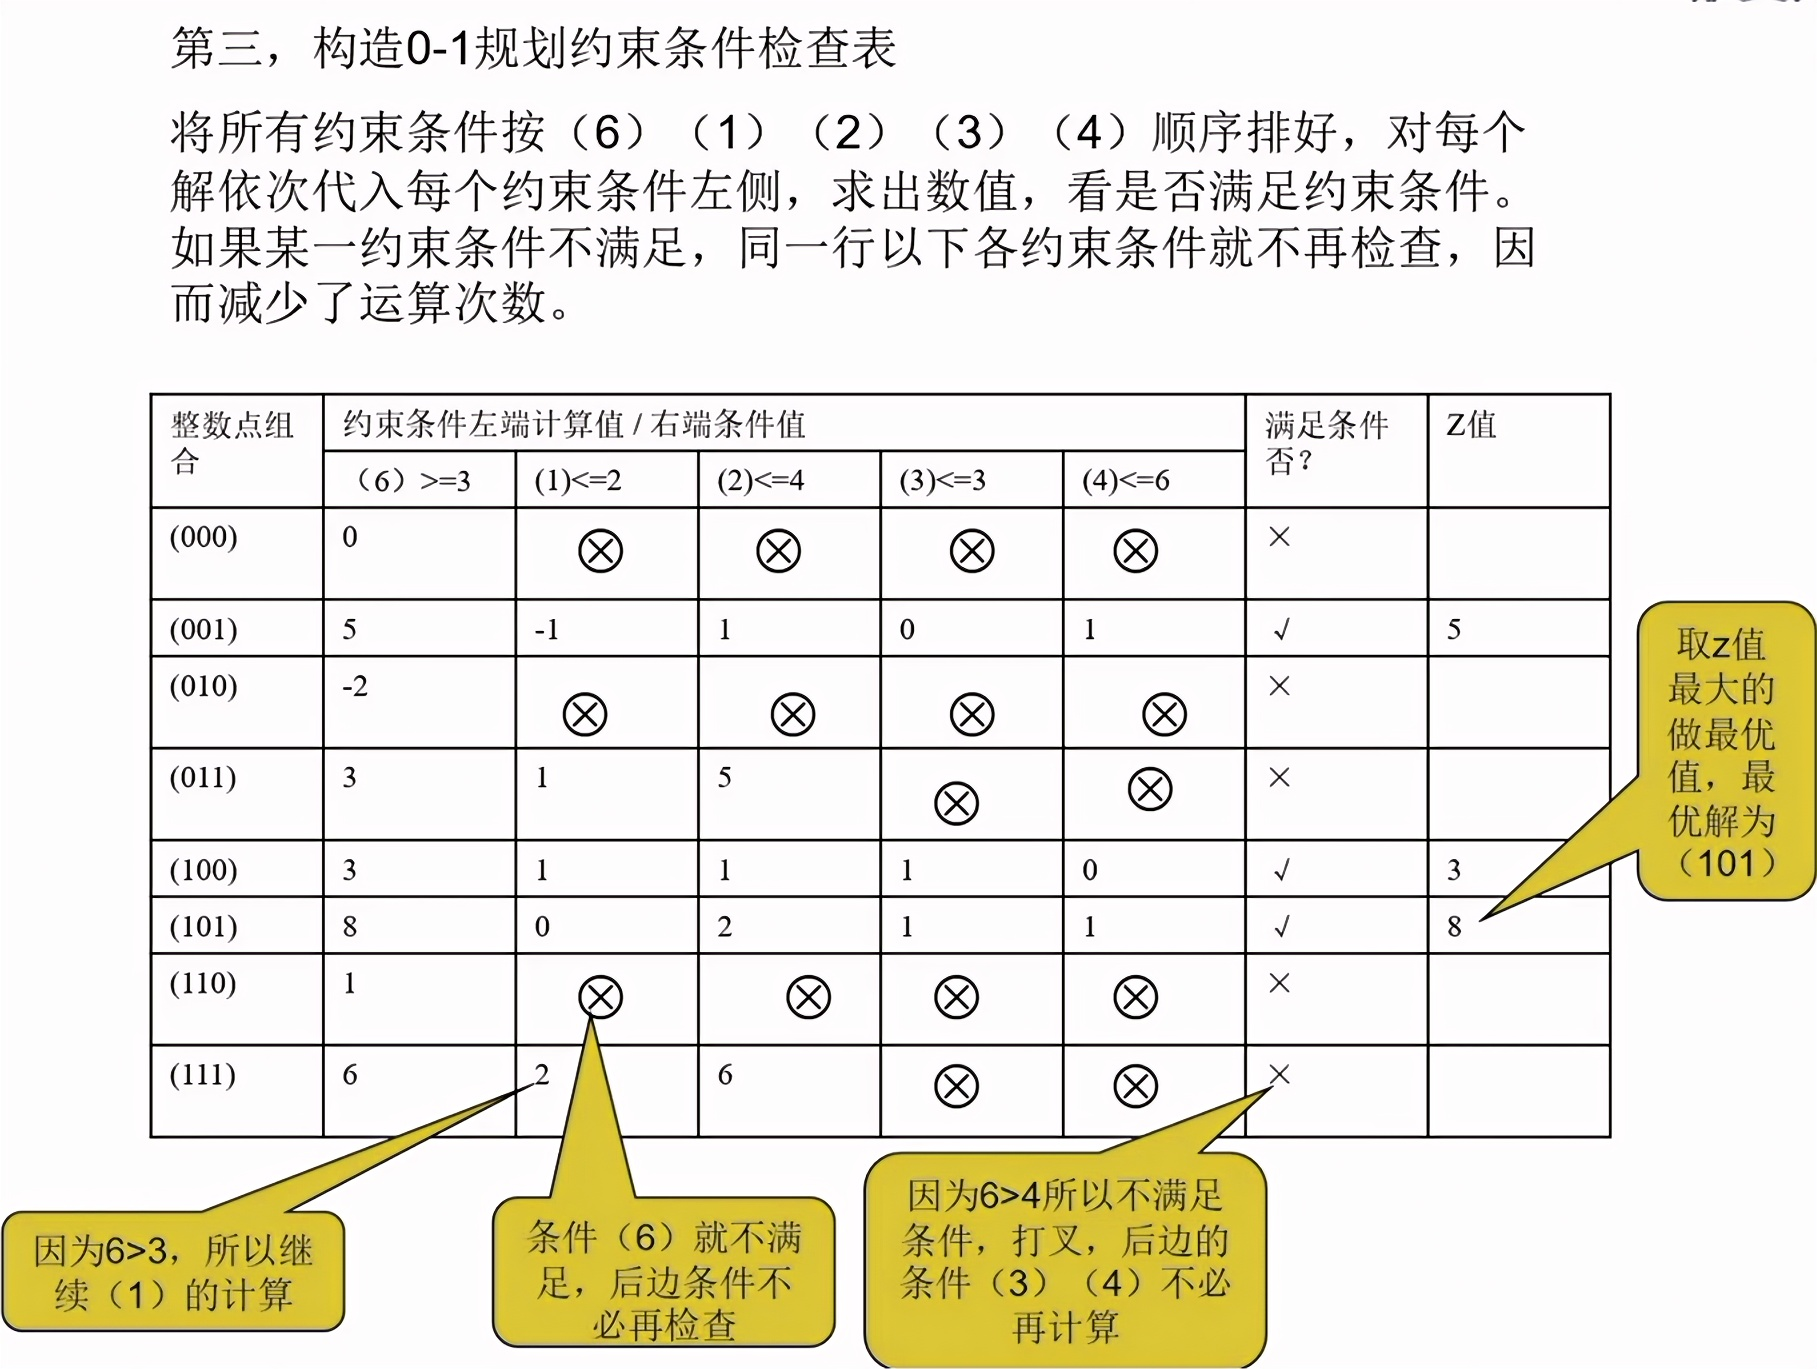
\includegraphics[width=0.8\textwidth]{./image/16.png}
            \caption{0-1规划约束条件检查表}
            \label{fig:Chapter4_Temporary_Pavilion_1}
        \end{figure}
    \end{exbox}







    \section{案例分析}
    \begin{exbox}{\textbf{生产计划问题}}
    1\textbf{例:}某工厂配套生产某种专业电子产品,今年前6个月收到的该产品的订货数量分别为 3000件,4500件,3500件,4000件,4000件和5000 件.已知该厂的正常生产能力为每月 3000件,利用加班生产还可以生产 1500 件.正常生产的成本为每件 5000 元,加班生产还要增加1500 元的成本,库存成本为每件每月200元.试问该厂如何组织安排生产才能在保证完成生产计划的情况下使生产成本最低?
    \textbf{解:} 根据这个问题的实际情况,设$x_i$表示第$i$个月正常生产的产品数量;
    $y_i$表示第$i$个月加班生产的产品数量;$z_i$表示第$i$个月月初产品的库存数量。
    $d_i$表示第$i$个月的需求量$(i=1,2,\cdots,6)$,并且第1个月月初的库存为 0,则问题的生产成本为:
    $$
        \sum_{i=1}^{6}(5000x_i+6500y_i+200z_i)
    $$
    三项分别为正常生产成本、加班生产成本和库存成本。
    \end{exbox}
    \begin{exbox}{\textbf{游泳队员分配问题}}
        1\textbf{例:}某游泳队拟选用 A,B,C,D 四名游泳运动员组成一个 4x100m 混合泳接力队,参加大型运动会,他们的100m自由泳,蛙泳,蝶泳,仰泳的成绩如下表 4.3 所示.A,B,C,D 四名运动员各自游什么姿势,才最有可能取得最好成绩?
        \begin{table}[H]
            \centering
            \label{tab:4.3}
            \renewcommand{\arraystretch}{1.5}
            \begin{tabular}{|c|c|c|c|c|}
                \hline
                & 自由泳 & 蝶泳 & 蛙泳 & 仰泳 \\ \hline
                A & 56 & 74 & 61 & 63 \\ \hline
                B & 63 & 69 & 65 & 71 \\ \hline
                C & 57 & 77 & 63 & 67 \\ \hline
                D & 55 & 76 & 62 & 62 \\ \hline
            \end{tabular}
            \caption{队员的游泳成绩}
        \end{table}
        \textbf{解:} 根据题意,假设问题的决策变量为 $x_{ij}$,令 $i$ 名队员游泳第 $j$ 种姿势,$x_{ij}$ 的取值如下:
        \[
        x_{ij} =
        \begin{cases}
        1, & \text{让} i \text{名队员游泳第} j \text{种姿势,} \\
        0, & \text{不让} i \text{名队员游泳第} j \text{种姿势.}
        \end{cases}
        \]
        其中 $i=1,2,3,4$ 分别表示自由泳、蛙泳、蝶泳、仰泳。根据问题的要求可知,四名运动员的成绩矩阵为

        \[
        A = \left( a_{y} \right)_{4 \times 4} =
        \begin{pmatrix}
        56 & 74 & 61 & 63 \\
        63 & 69 & 65 & 71 \\
        57 & 77 & 63 & 67 \\
        55 & 76 & 62 & 62
        \end{pmatrix}
        \]
        以 $4 \times 100m$ 混合泳所用的总时间最小为目标,以每名运动员游一个项目,每一个项目只能有一名运动员完成为约束,这是一个标准的分派问题。$4 \times 100m$ 混合泳所用的总时间为:

        \[
        T = \sum_{i=1}^4 \sum_{j=1}^4 a_{y} x_{ij}
        \]
        该模型为一个 $0-1$ 整数规划模型。

        \begin{align*}
            \text{min } T &= \sum_{i=1}^4 \sum_{j=1}^4 a_{y} x_{ij} \\
            \text{s.t.} \quad & \left\{
            \begin{aligned}
            \sum_{i=1}^4 x_{ij} &= 1, \quad (j=1,2,3,4) \\
            \sum_{j=1}^4 x_{ij} &= 1, \quad (i=1,2,3,4) \\
            x_{ij} &= 0 \text{ 或 } 1, \quad (i,j=1,2,3,4)
            \end{aligned}
            \right.
        \end{align*}

    \end{exbox}
\ifx\allfiles\undefined
	
	% 如果有这一部分的参考文献的话,在这里加上
	% 没有的话不需要
	% 因此各个部分的参考文献可以分开放置
	% 也可以统一放在主文件末尾。
	
	%  bibfile.bib是放置参考文献的文件,可以用zotero导出。
	% \bibliography{bibfile}
	
	end{document}
	\else
	\fi
    \ifx\allfiles\undefined

    % 如果有这一部分另外的package,在这里加上
    % 没有的话不需要
    
    \begin{document}
\else
\fi
\section{第四章作业}
\subsection{车间生产问题(分枝定界法)}
\textbf{Q:}设某服装加工厂有5个生产车间,可以用6种不同的成品布料(单位为m)加工不同的服装销售。对于第$i$个生产车间分别利用第$j$种布料进行加工生产后,可以获得利润为$r_{ij}$(元/m)$(i=1,2,...,5; j=1,2,...,6)$,具体的数据表如表4.5所示。\\
该厂现有资金40万元,为了分配这些资金,根据各车间的实际生产需求,工厂要求每个车间每种布料至少加工1000米,每个车间的总加工能力最多10000米,那么试问该工厂每种布料应购买多少米,又如何分配给所属的5个车间,使得总利润最大?

\begin{table}[ht]
\centering
\begin{tabular}{|c|c|c|c|c|c|c|}
\hline
\multirow{2}{*}{布料} & \multicolumn{6}{c|}{加工利润/元} \\ \cline{2-7} 
                      & 1 & 2 & 3 & 4 & 5 & 6 \\ \hline
车间一 & 4 & 3 & 4 & 4 & 5 & 6 \\ \hline
车间二 & 3 & 4 & 5 & 3 & 4 & 5 \\ \hline
车间三 & 5 & 3 & 4 & 5 & 5 & 4 \\ \hline
车间四 & 3 & 3 & 4 & 4 & 6 & 6 \\ \hline
车间五 & 3 & 3 & 3 & 4 & 5 & 7 \\ \hline
布料单价/元/米 & 6 & 6 & 7 & 8 & 9 & 10 \\ \hline
\end{tabular}
\caption{布料单价及加工利润}
\end{table}

\textbf{A:分析如下。}\\
为最大化服装加工厂的总利润,定义以下变量和参数:

\begin{itemize}
    \item 令$I = \{1, 2, 3, 4, 5\}$为车间集合
    \item 令$J = \{1, 2, 3, 4, 5, 6\}$为布料集合
    \item 令$x_{ij}$为车间$i$分配的布料$j$的米数(整数,单位:米)
    \item 令$r_{ij}$为车间$i$使用布料$j$的单位利润(元/米),由表4.5给出
    \item 令$c_j$为布料$j$的单价(元/米),由表4.5给出
\end{itemize}

\textbf{目标函数}\\
最大化总利润:
\[
\max z = \sum_{i=1}^5 \sum_{j=1}^6 r_{ij} x_{ij}
\]

\textbf{约束条件}
\begin{enumerate}
    \item 预算约束:
    \[
    \sum_{i=1}^5 \sum_{j=1}^6 c_j x_{ij} \leq 400000
    \]
    \item 最低加工量约束:
    \[
    x_{ij} \geq 1000 \quad \forall i = 1, 2, \ldots, 5; \quad \forall j = 1, 2, \ldots, 6
    \]
    \item 车间容量约束:
    \[
    \sum_{j=1}^6 x_{ij} \leq 10000 \quad \forall i = 1, 2, \ldots, 5
    \]
    \item 整数约束:
    \[
    x_{ij} \in \mathbb{Z}^+, \quad x_{ij} \geq 1000 \quad \forall i, j
    \]
\end{enumerate}

\begin{codebox}{Matlab代码(修正版)}{1}
\begin{verbatim}
% 服装加工厂整数规划问题求解
clear; clc;

% 定义参数
m = 5; % 车间数
n = 6; % 布料种类
total_var = m * n;

% 利润矩阵和单价
R = [4 3 4 4 5 6; 3 4 5 3 4 5; 5 3 4 5 5 4; 
     3 3 4 4 6 6; 3 3 3 4 5 7];
c = [6 6 7 8 9 10];

% 目标函数
f = -R(:);

% 约束构造
A = zeros(m+1, total_var);
b = zeros(m+1, 1);

% 预算约束
A(1,:) = repelem(c, 1, m);
b(1) = 400000;

% 车间容量约束(修正关键错误)
for i = 1:m
    A(i+1, i:m:end) = 1; % 正确索引每个车间的所有布料
    b(i+1) = 10000;
end

% 变量范围
lb = 1000 * ones(total_var, 1);
ub = inf(total_var, 1);
intcon = 1:total_var;

% 求解
[x, fval] = intlinprog(f, intcon, A, b, [], [], lb, ub);

% 结果输出
x = reshape(x, [m, n]);
total_profit = -fval;
fprintf('最大总利润: %.2f元\n', total_profit);
disp('布料分配方案(x_ij, 单位:米):'); disp(x);

% 每种布料购买量
fabric_amount = sum(x, 1);
fprintf('每种布料购买量(米):\n');
for j = 1:n
    fprintf('布料%d: %.0f米\n', j, fabric_amount(j));
end
\end{verbatim}
\end{codebox}

\textbf{求解方法}\\
采用分枝定界法求解该整数规划问题。通过MATLAB的\texttt{intlinprog}函数实现,关键修正在于车间容量约束的索引方式,确保正确限制每个车间的总加工量。

\textbf{实验结果}
\begin{itemize}
    \item \textbf{最大总利润}:243,000元
    \item \textbf{布料分配方案}(单位:米):
    \[
    \begin{bmatrix}
    1000 & 1000 & 1000 & 1000 & 1000 & 5000 \\
    1000 & 1000 & 5000 & 1000 & 1000 & 1000 \\
    5000 & 1000 & 1000 & 1000 & 1000 & 1000 \\
    1000 & 1000 & 1000 & 1000 & 3000 & 3000 \\
    1000 & 5000 & 1000 & 1000 & 1000 & 1000
    \end{bmatrix}
    \]
    \item \textbf{每种布料购买量}:
    \begin{itemize}
        \item 布料1:9000米
        \item 布料2:9000米
        \item 布料3:9000米
        \item 布料4:5000米
        \item 布料5:7000米
        \item 布料6:15000米
    \end{itemize}
\end{itemize}

\textbf{结果验证}
\begin{itemize}
    \item \textbf{预算约束}:总成本$=9000\times6+9000\times6+9000\times7+5000\times8+7000\times9+15000\times10=400,000$元,满足
    \item \textbf{最低加工量}:所有$x_{ij} \geq 1000$,满足
    \item \textbf{车间容量}:各车间总量均为10,000米(如车间5:$1000+5000+1000+1000+1000+1000=10,000$),满足
    \item \textbf{利润验证}:车间4利润$=3\times1000+3\times1000+4\times1000+4\times1000+6\times3000+6\times3000=52,000$元,总利润243,000元验证通过
\end{itemize}

\subsection{旅行者背包问题(0-1规划)}
\textbf{Q:}首先列写模型,然后自己赋值进行程序求解如下题目:一个旅行者要在背包里装一些最有用的东西,但限制最多只能携带 bkg 件物品,每件物品只能是整件携带,对每件物品都规定了一定的“使用价值”(有用的程度),如果共有 n 件物品,第 j 件物品重 $a_j$ kg,其价值为 $c_j (j=1,2,…,n)$,问题是:在携带的物品总重量不超过 bkg 的条件下,携带哪些物品可使总价值最大?
\\
\textbf{A:分析如下。}
\textbf{数学模型}\\
定义以下变量和参数:
\begin{itemize}
    \item \( n \):物品总数。
    \item \( b \):背包最大承重量。
    \item \( a_j \):第 \( j \) 件物品的重量。
    \item \( c_j \):第 \( j \) 件物品的价值。
    \item \( x_j \):二元变量,表示是否携带第 \( j \) 件物品(\( x_j = 1 \) 表示携带,\( x_j = 0 \) 表示不携带)。
\end{itemize}

\textbf{目标函数}:
\[
\max z = \sum_{j=1}^n c_j x_j
\]

\textbf{约束条件}:
\begin{enumerate}
    \item 重量约束:
    \[
    \sum_{j=1}^n a_j x_j \leq b
    \]
    \item 二元约束:
    \[
    x_j \in \{0, 1\} \quad \forall j = 1, 2, \ldots, n
    \]
\end{enumerate}

\textbf{具体实例}\\
我们选择以下数据:
\begin{itemize}
    \item \( n = 5 \)(物品总数)。
    \item \( b = 10 \)(背包最大承重)。
    \item 物品的重量和价值如下:
\end{itemize}

\begin{center}
\begin{tabular}{|c|c|c|}
\hline
\( j \) & \( a_j \) (kg) & \( c_j \) \\
\hline
1 & 2 & 3 \\
2 & 3 & 4 \\
3 & 4 & 5 \\
4 & 5 & 6 \\
5 & 6 & 7 \\
\hline
\end{tabular}
\end{center}

\textbf{MATLAB代码}\\
以下是使用显枚举法求解的MATLAB代码:

\begin{codebox}{显枚举法Matlab代码}{1}
\begin{amzcode}{matlab}
% 0-1背包问题求解(显枚举法)
clear; clc;

% 参数定义
n = 5; % 物品总数
b = 10; % 背包最大承重
a = [2, 3, 4, 5, 6]; % 物品重量
c = [3, 4, 5, 6, 7]; % 物品价值

% 初始化变量
max_val = 0; % 最大价值
best_comb = []; % 最优组合

% 枚举所有可能的组合
for i = 0:2^n - 1
    comb = zeros(1,n); % 当前组合
    for j = 1:n
        comb(j) = bitget(i,j); % 使用bitget获取二进制表示
    end
    total_weight = sum(a .* comb); % 计算总重量
    if total_weight <= b % 如果总重量不超过背包容量
        total_value = sum(c .* comb); % 计算总价值
        if total_value > max_val % 更新最大价值和最优组合
            max_val = total_value;
            best_comb = comb;
        end
    end
end

% 输出结果
fprintf('最大价值: %d\n', max_val);
fprintf('选中的物品: ');
for j = 1:n
    if best_comb(j) == 1
        fprintf('%d ', j);
    end
end
fprintf('\n');
\end{amzcode}
\end{codebox}

\begin{codebox}{动态规划法Matlab代码}{1}
	\begin{amzcode}{matlab}
% 动态规划法求解
dp = zeros(n+1, b+1); % 初始化dp表
for i = 1:n
    for w = 0:b
        idx_w = w + 1; % MATLAB索引从1开始
        if a(i) > w
            dp(i+1, idx_w) = dp(i, idx_w); % 不能携带第i件物品
        else
            take = dp(i, idx_w - a(i)) + c(i); % 携带第i件物品
            not_take = dp(i, idx_w); % 不携带第i件物品
            dp(i+1, idx_w) = max(take, not_take); % 取最大值
        end
    end
end
max_val_dp = dp(n+1, b+1); % 获取最大价值
fprintf('动态规划法最大价值: %d\n', max_val_dp);
\end{amzcode}
\end{codebox}

\textbf{求解方法}\\
采用显枚举法求解该0-1背包问题。由于物品数量较少(\( n = 5 \)),共有 \( 2^5 = 32 \) 种组合,显枚举法计算复杂度可接受。求解步骤如下:
\begin{enumerate}
    \item 枚举所有可能的物品组合(使用二进制表示,从 \( 0 \) 到 \( 2^n - 1 \))。
    \item 对每种组合,计算总重量 \( \sum_{j=1}^n a_j x_j \),检查是否满足 \( \leq b \)。
    \item 若满足重量约束,计算总价值 \( \sum_{j=1}^n c_j x_j \),更新最大价值和最优组合。
    \item 输出最大价值和选中的物品。
\end{enumerate}
为验证结果,采用动态规划法,通过构建二维表格 \( dp \),计算前 \( i \) 件物品在容量 \( w \) 下的最大价值,确保结果正确。

\textbf{MATLAB代码思路}\\
MATLAB代码通过以下步骤实现:
\begin{itemize}
    \item \textbf{参数初始化}:定义物品数量(\( n = 5 \))、背包容量(\( b = 10 \))、物品重量数组 \( a \)、价值数组 \( c \)。
    \item \textbf{显枚举法}:
        \begin{itemize}
            \item 使用循环遍历 \( 0 \) 到 \( 2^n - 1 \),通过二进制位提取每种组合。
            \item 计算每种组合的总重量和总价值,筛选满足重量约束的组合。
            \item 记录最大价值和对应的物品组合。
        \end{itemize}
    \item \textbf{动态规划法}:
        \begin{itemize}
            \item 构建二维数组 \( dp \),其中 \( dp[i][w] \) 表示前 \( i \) 件物品在容量 \( w \) 下的最大价值。
            \item 使用递推公式更新 \( dp \),比较携带和不携带第 \( i \) 件物品的价值。
        \end{itemize}
    \item \textbf{求解与输出}:输出显枚举法的最优解(最大价值和选中的物品),并用动态规划法验证最大价值。
\end{itemize}

\textbf{实验结果}\\
运行MATLAB代码,得到以下结果:
\begin{itemize}
    \item \textbf{最大价值}:13
    \item \textbf{选中的物品}:物品 1, 2, 4
    \item \textbf{动态规划验证}:最大价值为 13,与显枚举法一致。
\end{itemize}

\textbf{结果验证}
\begin{itemize}
    \item \textbf{重量约束}:选中的物品 1、2、4 的总重量为 \( 2 + 3 + 5 = 10 \leq 10 \),满足约束。
    \item \textbf{价值计算}:总价值为 \( 3 + 4 + 6 = 13 \),与输出一致。
    \item \textbf{其他组合验证}:
        \begin{itemize}
            \item 物品 1、2、3:重量 \( 2 + 3 + 4 = 9 \leq 10 \),价值 \( 3 + 4 + 5 = 12 < 13 \)。
            \item 物品 3、5:重量 \( 4 + 6 = 10 \leq 10 \),价值 \( 5 + 7 = 12 < 13 \)。
            \item 物品 2、4:重量 \( 3 + 5 = 8 \leq 10 \),价值 \( 4 + 6 = 10 < 13 \)。
        \end{itemize}
    \item \textbf{动态规划验证}:动态规划法计算的最大价值为 13,与显枚举法结果一致。
\end{itemize}

\ifx\allfiles\undefined
    
    % 如果有这一部分的参考文献的话,在这里加上
    % 没有的话不需要
    % 因此各个部分的参考文献可以分开放置
    % 也可以统一放在主文件末尾。
    
    %  bibfile.bib是放置参考文献的文件,可以用zotero导出。
    % \bibliography{bibfile}
    
    end{document}
    \else
    \fi
    \ifx\allfiles\undefined

	% 如果有这一部分另外的package,在这里加上
	% 没有的话不需要
	
	\begin{document}
\else
\fi
    \chapter{非线性规划}
    \section{非线性规划问题与数学模型}
    \subsection{非线性规划问题的定义}
    
\begin{dfnbox}{非线性规划}{amznotes}
    如果目标函数或约束条件方程中存在任何非线性因子,则问题\textbf{非线性规划}。
\end{dfnbox}
非线性规划具有以下几个特点:
\begin{itemize}
    \item 目标函数或约束条件方程中存在任何\textcolor{red}{非线性因子},或全部为\textcolor{red}{非线性函数}:
    \item \textcolor{red}{没有统一的、通用的解法}(这不同于线性规划,它有单纯形法作为通用解法),目前各种解法都有自己的适用范围;
    \item 非常难以采用解析解法,更多采用\textcolor{red}{数值解法};
    \item 非线性规划的最优解不像线性规划那样在边界点达到,而是\textcolor{red}{有可能在可行域中任一点}达到;
    \item 非线性规划存在\textcolor{red}{局部极值点}和\textcolor{red}{全局极值点}之分,这一点也与线性规划不同。
\end{itemize}
\begin{dfnbox}{局部极值点}{amznotes}
    设 $x^* \in K$,如果存在某个 $\epsilon > 0$,使得有与 $x$ 距离小于 $\epsilon$ 的 $x \in K$(即 $x \in K \cap \|x - x^*\| < \epsilon$),均满足不等式 $f(x) \geq f(x^*)$,则称 $x^*$ 为 $f(x)$ 在 $K$ 上的局部极小点,$f(x^*)$ 为局部极小值。\\
    若 $x \neq x^*$ 且 $f(x) > f(x^*)$,则 $x^*$ 为严格局部极小点,$f(x^*)$ 为严格局部极小值。
\end{dfnbox}
\begin{dfnbox}{全局极值点}{amznotes}
    设 $x^* \in K$,如果对于任意 $x \in K$,都有 $f(x) \geq f(x^*)$,则称 $x^*$ 为 $f(x)$ 在 $K$ 上的全局极小点,$f(x^*)$ 为全局极小值。\\
    若 $x \neq x^*$ 且 $f(x) > f(x^*)$,则 $x^*$ 为严格全局极小点,$f(x^*)$ 为严格全局极小值。
\end{dfnbox}
两点说明:
\begin{itemize}
    \item 局部极值点和全局极值点在定义上的主要区别是点的比较范围是x*附近的一个小邻域,还是整个K域。
    \item 局部极小点可能同时是全局极小点,全局极小点同时一定是局部极小点。
\end{itemize}
\begin{figure}[H]
    \centering
    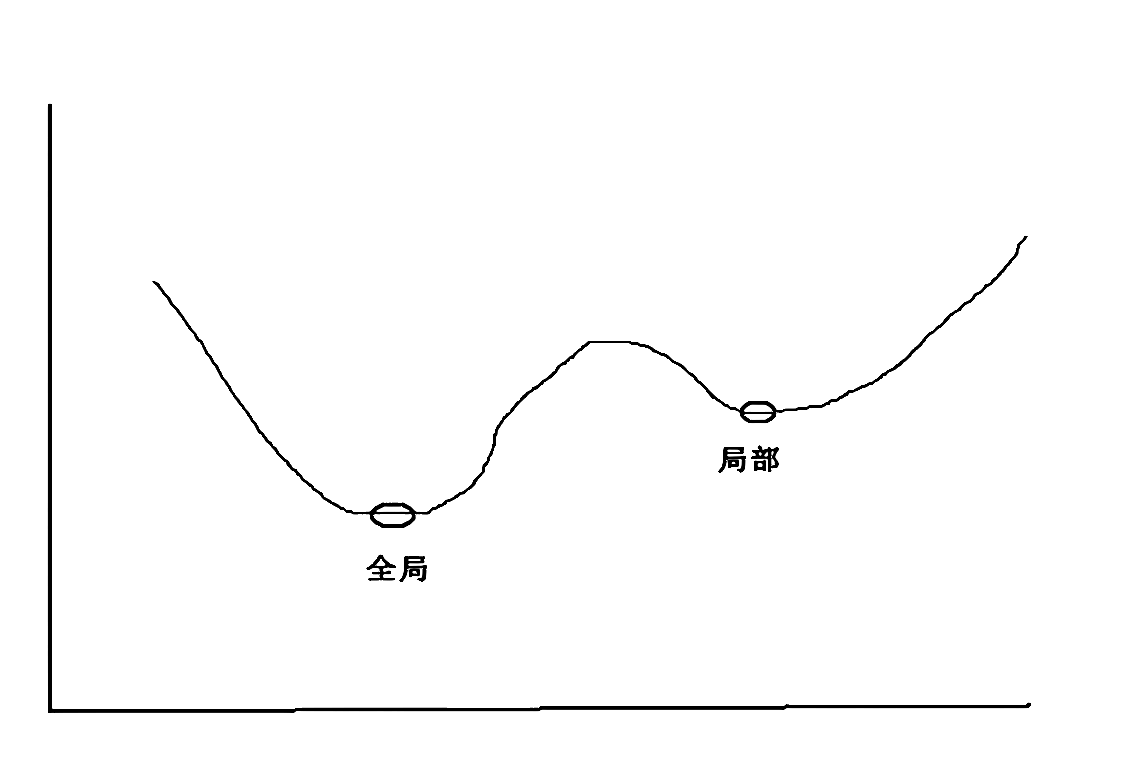
\includegraphics[width=0.5\textwidth]{./image/19.png}
    \caption{非线性规划也有局部极值和全局极值的区分}
    \label{fig:Chapter4_Temporary_Pavilion_1}
\end{figure}
\begin{figure}[H]
    \centering
    \begin{subfigure}{0.42\textwidth}
        \centering
        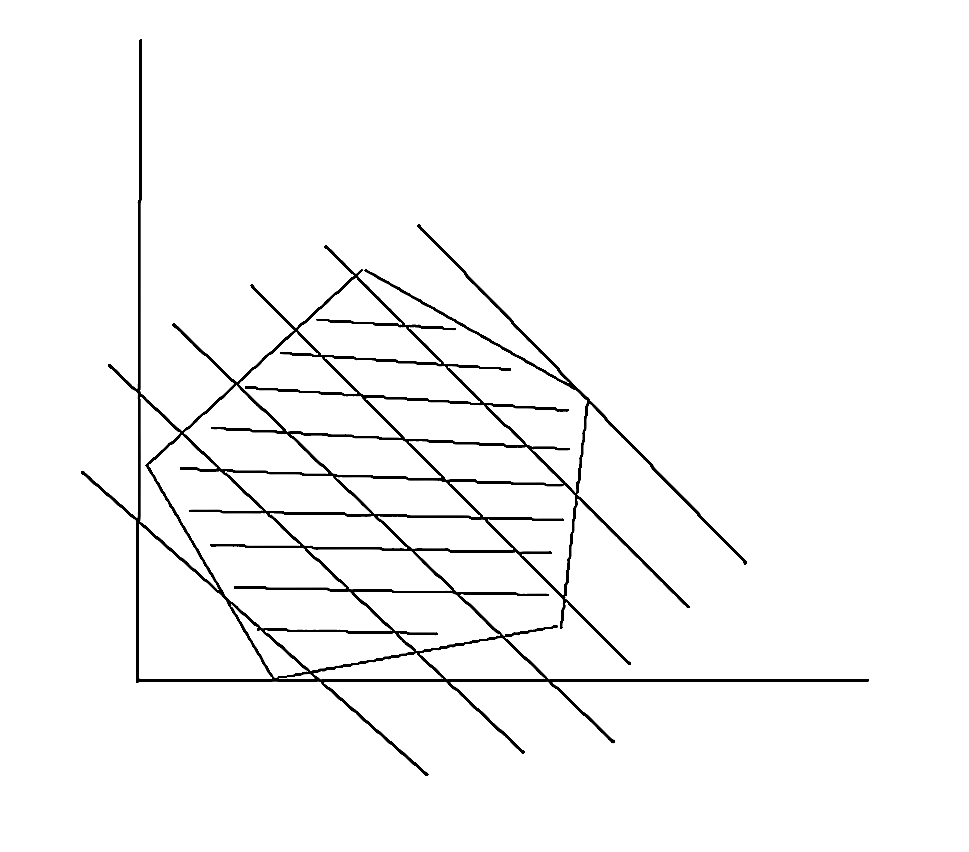
\includegraphics[width=\linewidth]{image/17.png}
        \caption{线性规划中,当目标函数取定值时,其等值几何图形为直线或平面。}
    \end{subfigure}
    \hfill
    \begin{subfigure}{0.4\textwidth}
        \centering
        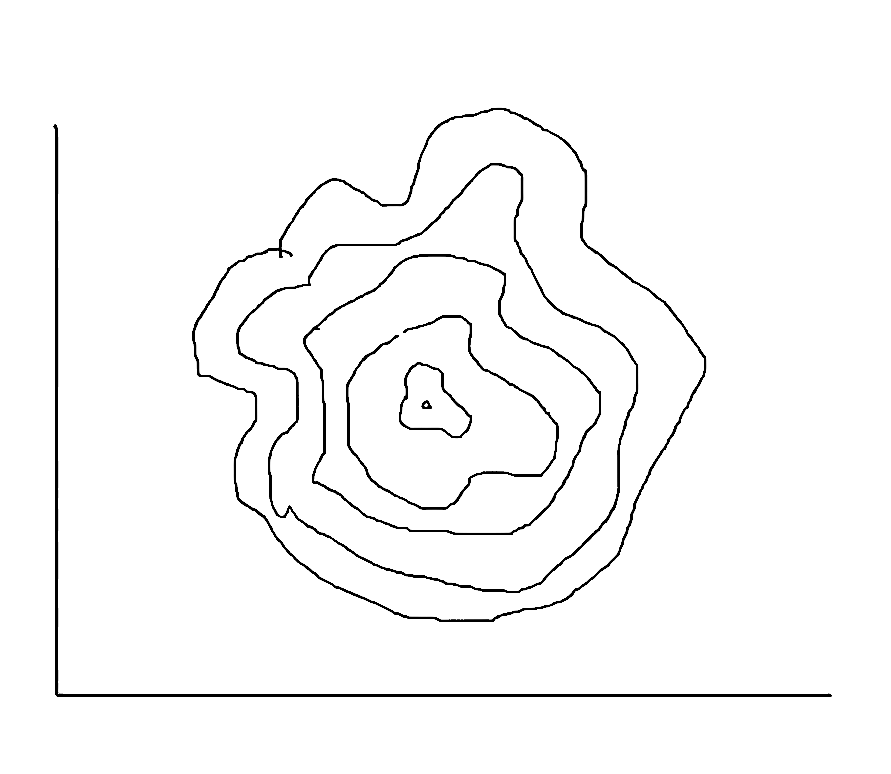
\includegraphics[width=\linewidth]{image/18.png}
        \caption{非线性规划中,等值线为规则或不规则的曲线、曲面,类似于地图上的等高线}
    \end{subfigure}
    \caption{线性规划与非线性规划的对比}
\end{figure}

\begin{exbox}{资源分配问题}
1\textbf{例:}有 A 和 B 两种资源,数量分别为 a 和 b,用于生产 n 种产品。如果 A 种资源以数量 \(x_k\),B 种资源以数量 \(y_k\),用于生产第 k 种产品,其收益为 \(g_k(x_k, y_k)\),问如何分配这两种资源用于 n 种产品的生产使总收益最大?
\\
\textbf{解:}

由题意,以 \(x_k\) 和 \(y_k\)(\(k = 1, 2, \dots, n\))为决策变量,以生产 n 种产品的总收益为目标函数,资源的总量为约束条件,则问题的优化模型为:

\[
\max z = g_1(x_1, y_1) + g_2(x_2, y_2) + \dots + g_n(x_n, y_n)
\]

约束条件:

\[
\begin{cases}
x_1 + x_2 + \dots + x_n = a, \\
y_1 + y_2 + \dots + y_n = b, \\
x_k \geq 0, \quad y_k \geq 0 \quad (k = 1, 2, \dots, n).
\end{cases}
\]
\end{exbox}

\begin{exbox}{最小圆盘问题}
    1\textbf{例:}设平面上有 $m$ 个点,找覆盖这 $m$ 个点的最小圆盘。

    \textbf{解:} 设 $m$ 个点为 $p_i, \, i = 1, 2, \dots, m$,则平面上任一点 $x$ 到这 $m$ 个点的距离最大者满足
    
    \[
    f(x) = \max_{1 \leq i \leq m} \| x - p_i \|
    \]
    
    则以 $x$ 为圆心,$f(x)$ 为半径的圆盘必覆盖这 $m$ 个点,于是问题转化为求解最小半径的圆盘问题:
    
    \[
    \min_x \max_{1 \leq i \leq m} \| x - p_i \|
    \]
    
    这是一个无约束的非线性规划问题。
\end{exbox}
\textcolor{red}{若没有约束条件,称为无约束极值问题。否则称为约束极值问题。}
\subsection{非线性规划问题的数学模型}
\begin{thmbox}{一般形式}{cool}
    \begin{align*}
        \text{max} \quad & z = g_1(x_1, y_1) + g_2(x_2, y_2) + \cdots + g_n(x_n, y_n) \\
        \text{subject to} \quad & \sum_{k=1}^{n} x_k = a, \\
        & \sum_{k=1}^{n} y_k = b, \\
        & x_k \geq 0, \ y_k \geq 0 \quad (k = 1, 2, \dots, n).
        \end{align*}
        
        \begin{align*}
        \text{min} \quad & \max_{1 \leq l \leq m} \left\{ \| x - p_l \| \right\}
    \end{align*}
\end{thmbox}
\begin{thmbox}{标准模型I}{cool}
    \begin{align*}
        \min \quad & f(x) \\
        \text{subject to} \quad & h_i(x) = 0, \quad i = 1, 2, \dots, m \quad \text{(m 个等式约束)} \\
        & g_j(x) \geq 0, \quad j = 1, 2, \dots, l \quad \text{(l 个不等式约束)} \\
        & x \in \mathbb{R}^n
        \end{align*}
        
        \bigskip
        \text{若有另一种形式,可以转化为上述形式,例如:}
        \begin{align*}
        \max \quad  f(x) \quad &\Rightarrow \quad \min (-f(x)) \\
        g_j(x) \leq 0  \quad &\Rightarrow \quad -g_j(x) \geq 0
        \end{align*}
\end{thmbox}
\begin{thmbox}{标准模型II}{cool}
    \begin{align*}
        \min \quad & f(x) \\
        \text{subject to} \quad & g_i(x) \geq 0, \quad i = 1, 2, \dots, n \quad \text{(n 个不等式约束)} \\
        & x \in \mathbb{R}^n
    \end{align*}
\end{thmbox}


\begin{notebox}{\textbf{模型 I 与模型 II 的转换:}}
\\
主要是把等式约束化为不等式约束:
\begin{align*}
    h_i(x) = 0 \quad \Rightarrow \quad \begin{cases}
        h_i(x) \geq 0 \\
        h_i(x) \leq 0 \quad \Rightarrow \quad -h_i(x) \geq 0
    \end{cases}
    \Rightarrow
    g_i(x)\geq 0 
\end{align*}
\end{notebox}
\begin{notebox}{\textbf{求解方法}}
    \\求解非线性规划问题常有两种方法:
    \begin{enumerate}
        \item \textbf{解析法}:必要条件+充分条件;
        \item \textbf{数值法}:迭代。
    \end{enumerate}
\end{notebox}


\subsection{求解非线性规划问题的解析法}
为了使用解析方法解决非线性规划问题,我们首先引出几个定义\footnote{读者在微积分或数学分析课程中中学过以上概念。如果感到有些遗忘,可以理解为“梯度”就相当于一元函数的一阶导数,“Hesse 矩阵”就相当于一元函数的二阶导数。我们在判断一元函数的极值点的时候,就是通过求一阶导为0,二阶导大于或小于0来判断是极小值或极大值的。对于多元函数也是类似的道理。}:
\begin{dfnbox}{函数的梯度}{amznotes}
    设 $x \in K \subset \mathbb{R}^n$,$f(x)$ 在 $K$ 上有一阶连续偏导数,则
    \[
    \nabla f(x) \equiv \left[ \frac{\partial f(x)}{\partial x_1}, \frac{\partial f(x)}{\partial x_2}, \ldots, \frac{\partial f(x)}{\partial x_n} \right]^T
    \]
    称函数 $f(x)$ 在 $x$ 处的\textbf{梯度}。
\end{dfnbox}
\textbf{梯度的几何意义}:
    $\nabla f(x)$ 是 $f(x)$ 在 $x$ 处增加最快或减少最快的速度,也是 $f(x)$ 的图形在 $x$ 处的陡峭程度。
\begin{dfnbox}{平稳点}{amznotes}
    若$\nabla f(x)=0$,则称$x$是$f(x)$的\textbf{平稳点}。
\end{dfnbox}

\begin{dfnbox}{海森Hesse矩阵}{amznotes}
    设 $f(x)$ 在 $K$ 上有二阶连续偏导数,则
    \[
    H(x) \equiv \begin{bmatrix}
        \frac{\partial^2 f(x)}{\partial x_1^2} & \frac{\partial^2 f(x)}{\partial x_1 \partial x_2} & \cdots & \frac{\partial^2 f(x)}{\partial x_1 \partial x_n} \\
        \frac{\partial^2 f(x)}{\partial x_2 \partial x_1} & \frac{\partial^2 f(x)}{\partial x_2^2} & \cdots & \frac{\partial^2 f(x)}{\partial x_2 \partial x_n} \\
        \vdots & \vdots & \ddots & \vdots \\
        \frac{\partial^2 f(x)}{\partial x_n \partial x_1} & \frac{\partial^2 f(x)}{\partial x_n \partial x_2} & \cdots & \frac{\partial^2 f(x)}{\partial x_n^2}
    \end{bmatrix}
    \]
    称函数 $f(x)$ 在 $x$ 处的 \textbf{Hesse 矩阵}。
\end{dfnbox}
\begin{dfnbox}{矩阵的正定性,负定性,不定性}{amznotes}
    对于对称矩阵 $A$,若对任意非零向量 $X \neq 0$,二次型为正,即 $X^T A X > 0$,则称该二次型为正定二次型,$A$ 为正定矩阵\footnote{在线性代数中,我们学习过判断正定矩阵的方法有特征值判定法(所有特征值大于0)、主子式判定法(如果所有阶的顺序主子式,即从左上角开始的子矩阵的行列式都大于0);此外,如果两个矩阵都是正定的,那他们的和也是正定的;一个正定矩阵的逆矩阵也是正定的。}。\\
    若 $X^T A X \geq 0 \Rightarrow$ 半正定\\
    若 $X^T A X < 0 \Rightarrow$ 负定\\
    若 $X^T A X \leq 0 \Rightarrow$ 半负定\\
    若既非正定,又非负定,则为不定。
\end{dfnbox}
\begin{thmbox}{定理一:极值点必要条件}{cool}
    若$f(x)$在其存在一阶连续偏导数的区域内达到局部极值点,则该极值点必为平稳点。
\end{thmbox}
此处要注意:
\begin{itemize}
    \item 该定理是必要条件,反之不一定成立,即\textcolor{red}{平稳点不一定是极值点},例如鞍点。
    \item $f(x)$在其不满足一阶连续偏导数的区域内的极值点,不一定满足定理一。
\end{itemize}
\begin{figure}[H]
    \centering
    \begin{subfigure}{0.42\textwidth}
        \centering
        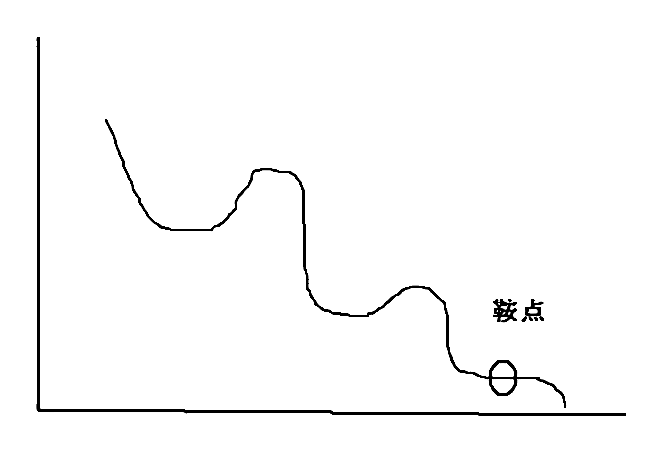
\includegraphics[width=\linewidth]{image/20.png}
        \caption{鞍点是平稳点但不是极值点}
    \end{subfigure}
    \hfill
    \begin{subfigure}{0.4\textwidth}
        \centering
        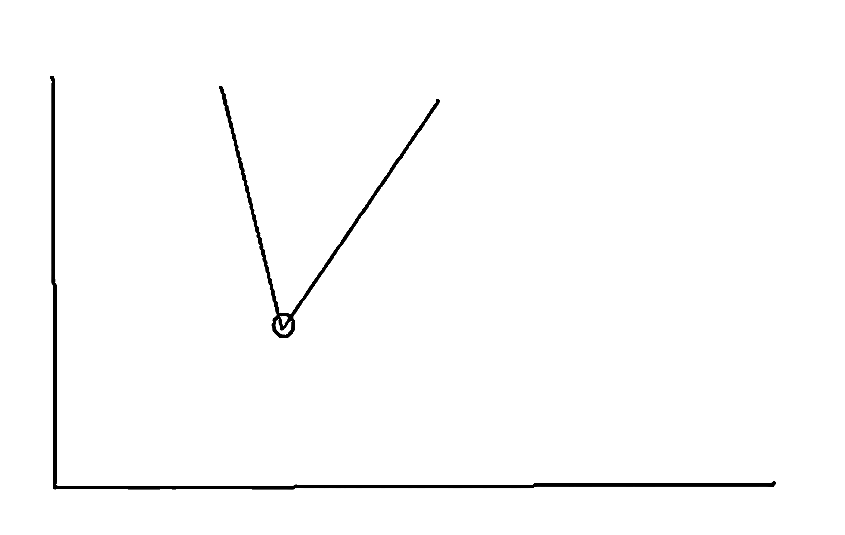
\includegraphics[width=\linewidth]{image/21.png}
        \caption{一阶偏导数不连续的极值点不一定是平稳点}
    \end{subfigure}
    \caption{定理一是必要条件的理解}
\end{figure}
为了能够正确判断极值点,我们使用定理二:
\begin{thmbox}{定理二:局部极值点判断的充要条件}{cool}
    若 $f(x)$ 在 $K$ 上具有二阶连续偏导数,并且满足:
    \begin{enumerate}
        \item $x^* \in K$ 是平稳点,即 $\nabla f(x^*) = 0$
        \item $H(x^*)$ 是正定矩阵(Hesse 矩阵)
    \end{enumerate}
    则 $x^* \in K$ 是 $f(x)$ 的严格局部极小点。
\end{thmbox}
\subsection{求解非线性规划问题的数值法}

\begin{dfnbox}{下降迭代算法}{amznotes}
    若由某算法产生的解序列 $\{ X^{(k)} \}$ 使目标函数值 $f(X^{(k)})$ 逐步减小,则称这组算法为\textbf{下降迭代算法}。
\end{dfnbox}

\begin{notebox}{\textbf{下降迭代算法}}{}
    \begin{itemize}
        \item \textbf{迭代法的基本思路:}
        \\
        初始估计 $X^{(0)}$ \quad $\xrightarrow{\text{按某种算法}}$ \quad 比 $X^{(0)}$ 更好的 $X^{(1)}$ \quad $\xrightarrow{\text{按算法}}$ \quad $X^{(2)} \cdots X^{(n)}$
        $\xrightarrow{\text{得到解序列}} \quad \{ X^{(0)}, X^{(1)}, \cdots, X^{(n)} \cdots \}$
    
        \bigskip
        若解序列收敛于 $X^*$,即,
        \[
        \lim_{k \to \infty} \| X^{(k)} - X^* \| = 0
        \]
        则称 $\{ X^{(0)}, X^{(1)}, \cdots, X^{(n)} \cdots \}$ 收敛于 $X^*$。
        \\
    \end{itemize}
\end{notebox}
几个关键问题是:
\begin{enumerate}
    \item 迭代算法的初始点 $X^{(0)}$ 的选择?
    \item 算法的设计,以当前点依据何种原则构建下一个点?
    \item 迭代算法的终止条件?
\end{enumerate}
\subsubsection{迭代法的基本步骤}
\begin{itemize}
\item \textbf{一、初值的确定}\\初值的确定没有特别的办法,很多情况下依靠经验,或求解者对问题的了解程度来确定的。初值应尽可能与可能的最优解靠得近一些。
\item \textbf{二、算法的设计}
\begin{enumerate}
    \item 选定某一初始点 $X^{(0)}$,并令 $k=0$。

    \item 确定能使 $f(X)$ 下降的搜索方向 $P^{(k)}$。

    \item 从 $X^{(k)}$ 出发行,沿方向 $P^{(k)}$ 确定迭代步长 $\lambda_k$。

    \item 确定,产生下一个迭代点 $X^{(k+1)}$,
    \[
    X^{(k+1)} = X^{(k)} + \lambda_k P^{(k)}.
    \]
    \item 检查新点$X^{k+1}$是否为极小点,或近似极小点,或满足规定的停止条件。
    \begin{itemize}
        \item 若是,则停止迭代;
        \item 否则,令 $k=k+1$,转(2)继续进行迭代。
    \end{itemize}
\end{enumerate}
\textcolor{red}{关键在于如何选取搜索方向 $P^{(k)}$ 和步长 $\lambda_k$}\footnote{各种迭代方法的差异主要就体现在这两者的选定上。}。
\\方向的确定相对困难,但很重要,避免南辕北辙。
\\步长的确定可见\hyperref[确定迭代步长的一维搜索方法]{确定迭代步长的一维搜索方法}和\hyperref[确定迭代步长的黄金分割法]{确定迭代步长的黄金分割法}。
\item \textbf{三、算法的结束条件}
\begin{itemize}
    \item 若算法优秀且收敛的极限值确为最优解,则能通过选代找到最优解。
    \item 若迭代步数有限,只能找到近似解,当满足所要求精度时,即停止迭代。
\end{itemize}
常用以下几个方法:
\begin{enumerate}
    \item \textbf{两次迭代值的绝对误差}
    \[
    \| X^{(k+1)} - X^{(k)} \| < \varepsilon_1
    \]
    \[
    | f(X^{(k+1)}) - f(X^{(k)}) | < \varepsilon_2
    \]

    \item \textbf{两次迭代值的相对误差}
    \[
    \frac{\| X^{(k+1)} - X^{(k)} \|}{\| X^{(k)} \|} < \varepsilon_1
    \]
    \[
    \frac{| f(X^{(k+1)}) - f(X^{(k)}) |}{| f(X^{(k)}) |} < \varepsilon_2
    \]

    \item \textbf{梯度条件}
    \[
    \| \nabla f(X^{(k)}) \| < \varepsilon
    \]
\end{enumerate}
\end{itemize}

\subsubsection{确定迭代步长的一维搜索方法}
\label{确定迭代步长的一维搜索方法}
\begin{notebox}{\textbf{一维、确定步长的三种方法}}
    \begin{enumerate}
        \item \textbf{恒定步长:} 步长每次不变,计算简单,但效果较差。

        \item \textbf{变步长:} 每次人工调整步长,效果较好,但实施麻烦,且需具备较多的经验。

        \item \textbf{最速下降步长:} 使沿搜索方向使目标函数值下降最多、最快,即沿射线 $X = X^{(k)} + \lambda P^{(k)}$ 求使目标函数 $f(X)$ 的极小,
        \[
        \lambda_k : \min f(X^{(k)} + \lambda P^{(k)}),
        \]
        由于这种方法是以$\lambda$为变量的元函数 $f(X^{(k)} + \lambda P^{(k)})$ 的极小点 $\lambda_k$,故称为一维搜索,这种确定的步长为\textbf{最佳步长}。
    \end{enumerate}
\end{notebox}
以下面这个草图为例,从零点出发,方向确定为横轴正方向了,如果在横轴上走出红色的步长,纵轴下降红色的部分;但是如果在横轴走出蓝色的步长,纵轴下降的部分就会更大。这就是先确定方向,沿着搜索方向使目标函数值下降最多。
\begin{figure}[H]
    \centering
    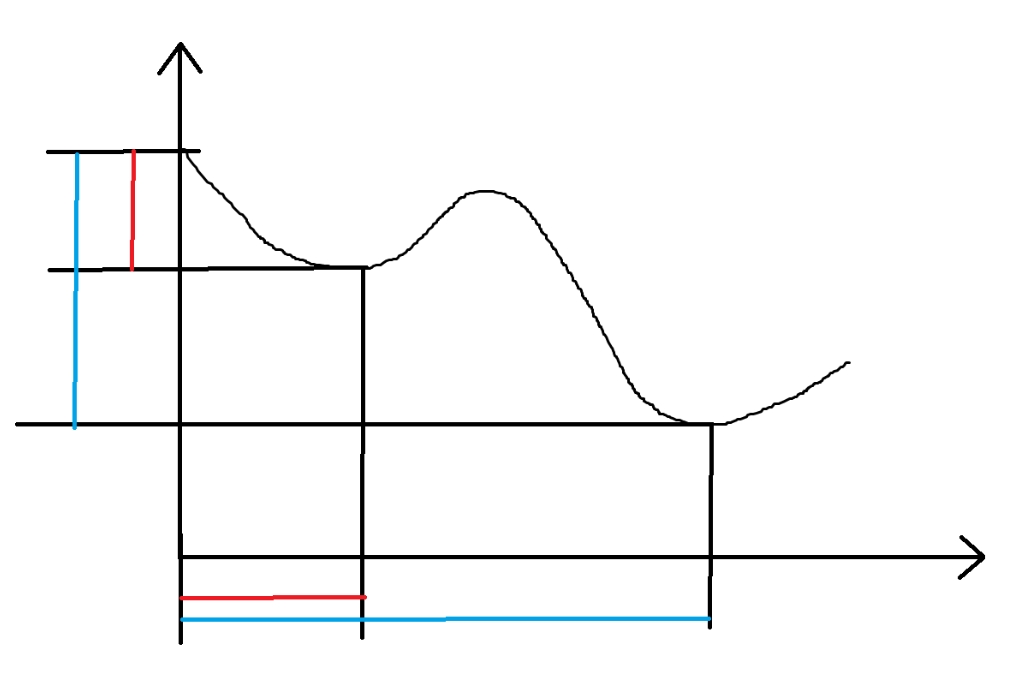
\includegraphics[width=0.35\textwidth]{./image/22.png}
    \caption{最速下降步长}
    \label{fig:Chapter4_Temporary_Pavilion_1}
\end{figure}
实际上,读者可能会想到,如果我们每次都要实时计算步长,岂不是降低了效率吗?这个问题是有道理的,请看下面的流程图:
\begin{figure}[H]
    \centering
    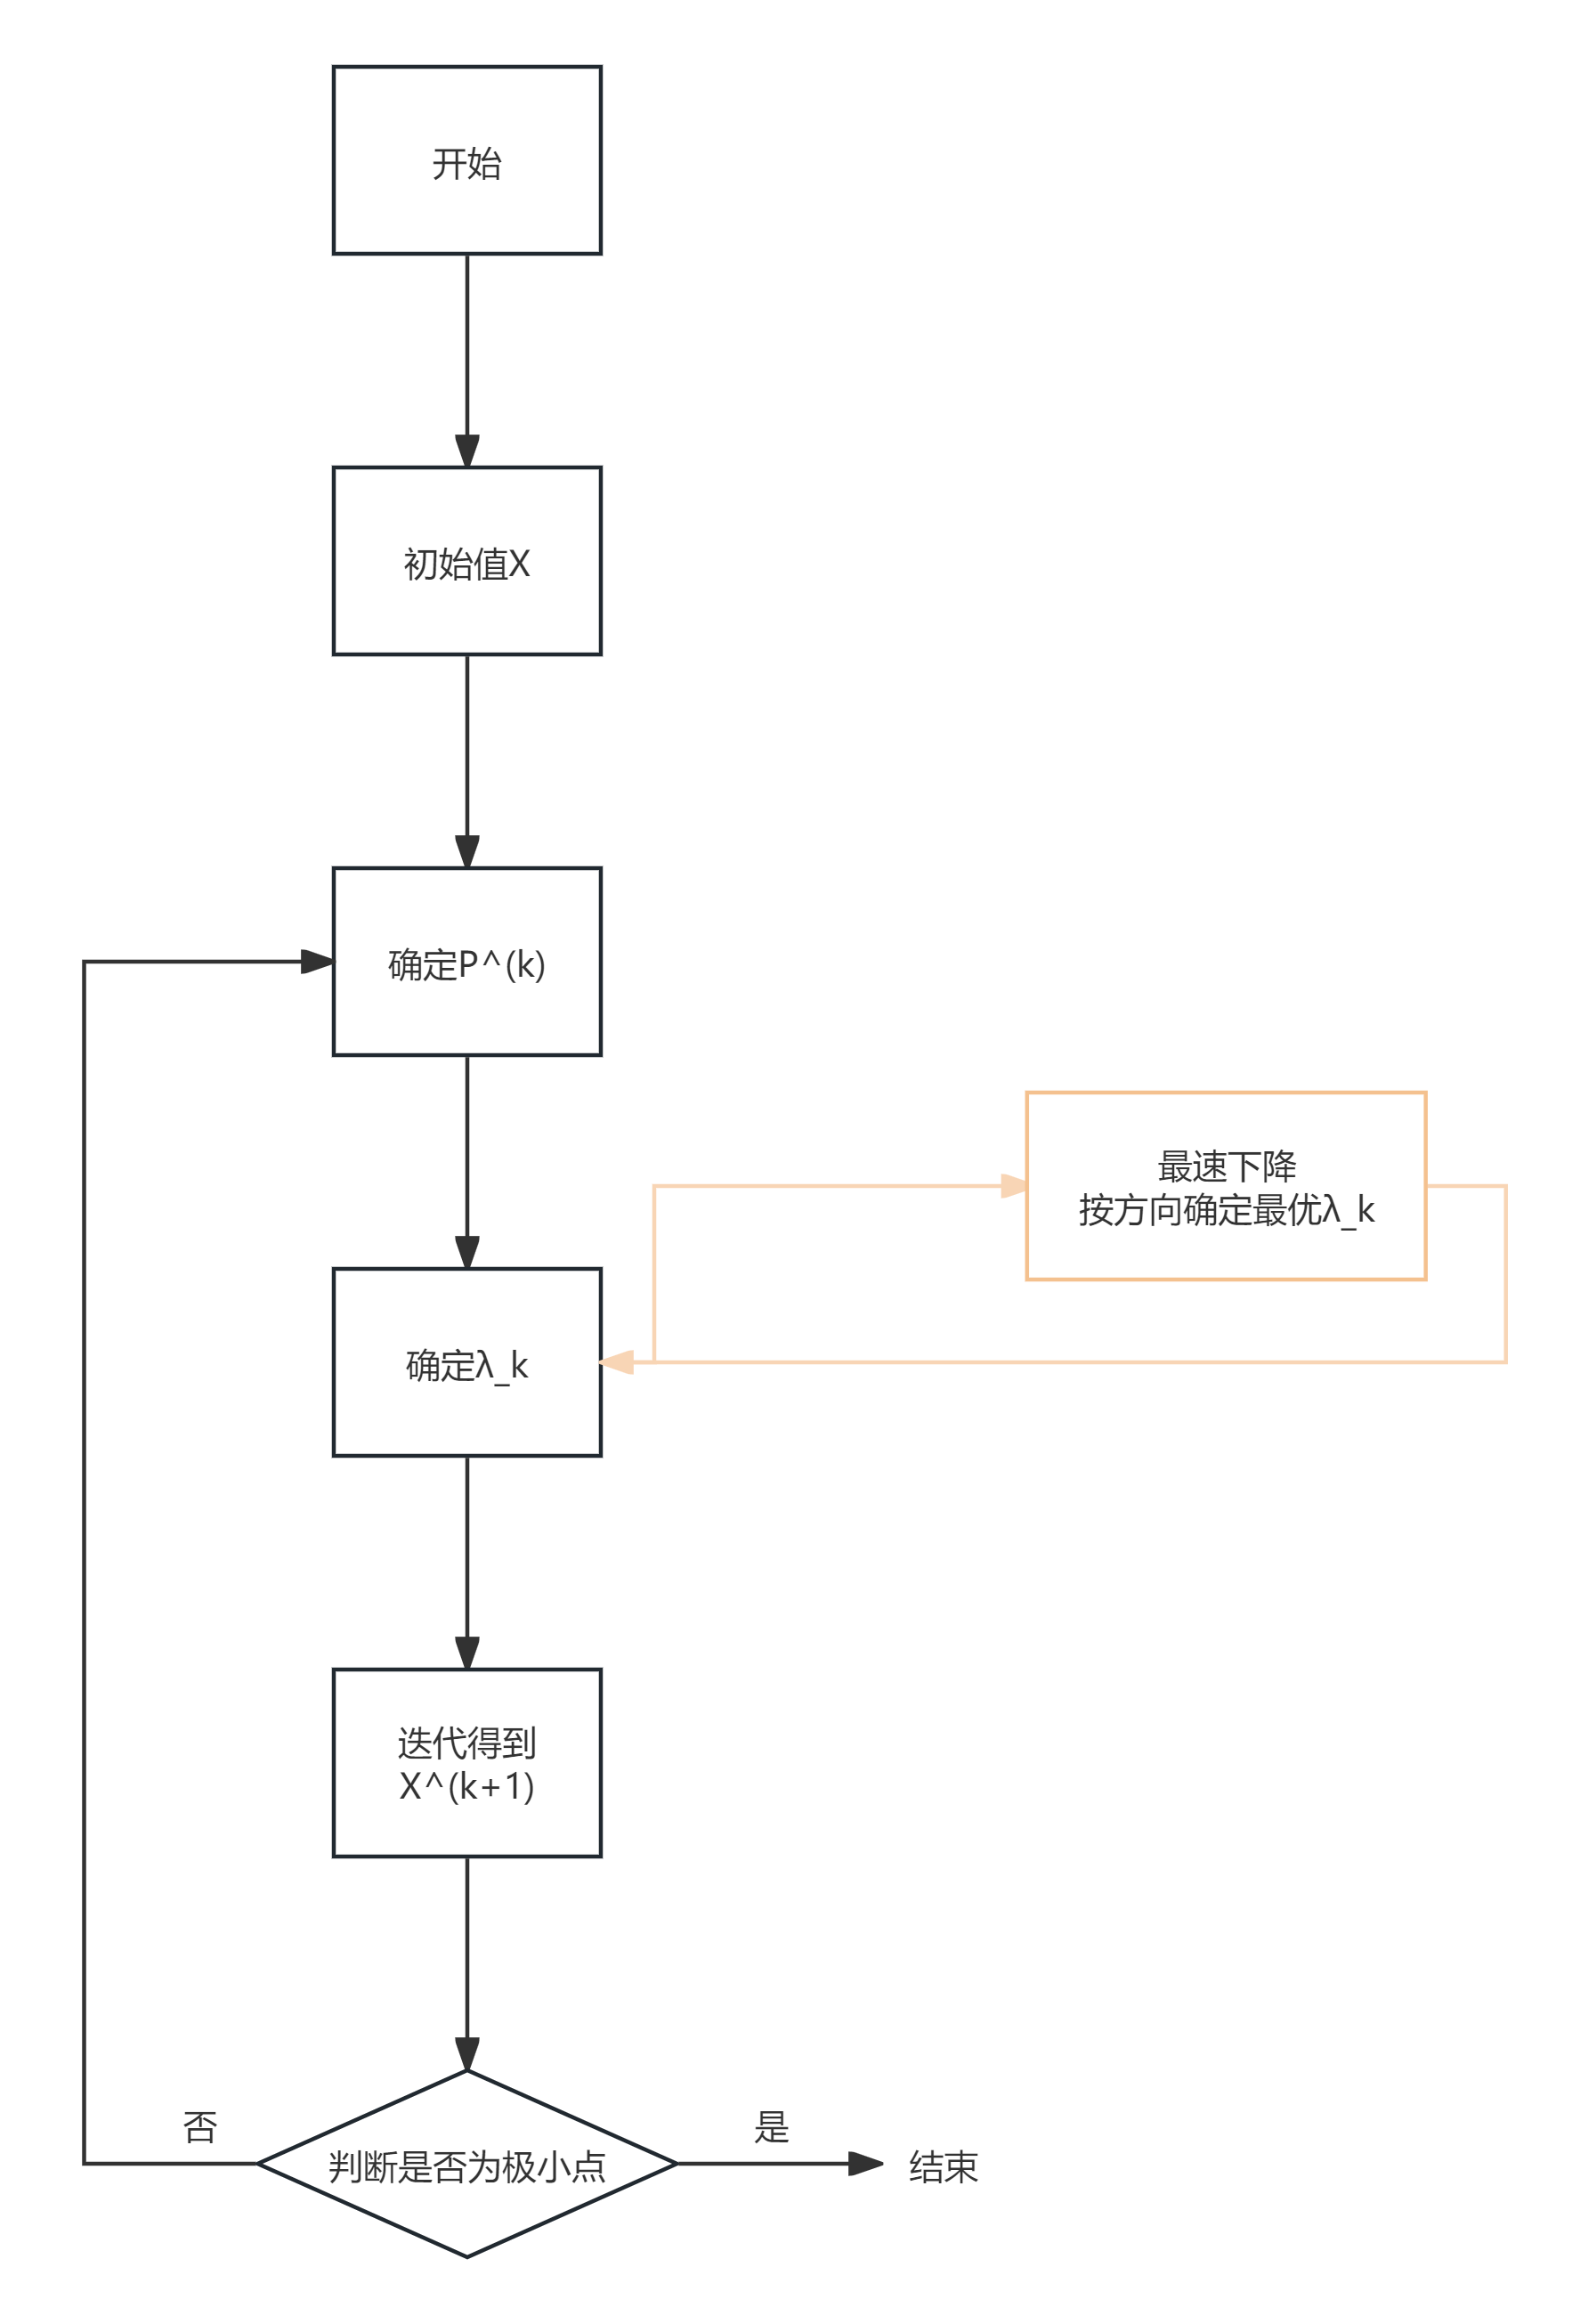
\includegraphics[width=0.6\textwidth]{./image/23.png}
    \caption{流程图}
    \label{fig:Chapter4_Temporary_Pavilion_1}
\end{figure}
引入\textcolor{orange}{橙色环节}之前,可能需要迭代100次,每次执行1秒;引入橙色环节之后,可能需要迭代50次,每次执行2秒。所以总的时间谁多谁少很难说了。因此我们想到,是否有办法在迭代过程中,既能带有最优步长的色彩,计算又不过于复杂?
\subsubsection{确定迭代步长的黄金分割法(0.618法)}
\label{确定迭代步长的黄金分割法}
\begin{notebox}{\textbf{黄金分割法(0.618 法)}}{}
    \\作为一种计算更简便的方法,黄金分割法在区间缩短效率上近似斐波那契法。
    \[
    x_k' = a_{k-1} + 0.382 [b_{k-1} - a_{k-1}]
    \]
    \[
    x_k'' = a_{k-1} + 0.618 [b_{k-1} - a_{k-1}]
    \]
    其中 $x_k'$ 和 $x_k''$ 分别是 $[a_{k-1}, b_{k-1}]$ 区间内的两个点,$0.382$ 和 $0.618$ 是黄金分割法的两个常数。
    可以这么理解:$x_k'$其实是$a_k$,$x_k''$其实是$b_k$,新的$\lambda_k$为$b_{k}-a_{k}$,旧的$\lambda_{k-1}$为$a_{k-1}-b_{k-1}$ 
\end{notebox}

\section{无约束非线性规划问题的解}
    \section{约束非线性规划问题(约束极值问题)}
    \section{案例分析}


\ifx\allfiles\undefined
	
	% 如果有这一部分的参考文献的话,在这里加上
	% 没有的话不需要
	% 因此各个部分的参考文献可以分开放置
	% 也可以统一放在主文件末尾。
	
	%  bibfile.bib是放置参考文献的文件,可以用zotero导出。
	% \bibliography{bibfile}
	
	end{document}
	\else
	\fi
    \ifx\allfiles\undefined

    % 如果有这一部分另外的package,在这里加上
    % 没有的话不需要
    
    \begin{document}
\else
\fi
\section{第五章作业}
\subsection{广告促销问题}
\textbf{Q:}某公司的营销管理员因经营需要,正在考虑如何安排两种不想管产品的促销活动,已知在两种产品的促销水平上的决策变量要受到资源的约束,假设用 x1, x2 表示两种产品促销活动的水平,则相应的约束为$4\mathrm{x}_1+x_2\leq20$和$\mathrm{x}_1+4x_2\leq20$,随着广告促销水平的增加,广告活动的回报会减少,从而想要取得同样程度销售增加量,就必须付出更多的广告成本。为此,营销管理员经过分析发现,对于产品1,当广告促销水平为$x$时,对应的收入为
$3x_{1}-(x_{1}-1)^{2}$(百万元);而产品2相应的收入为$3x_2-(x_2-2)^{2}$(百万元)。试为该公
司确定两种产品广告促销水平的最优组合。
\\
\textbf{A:分析如下。}

为最大化两种产品的总收入,定义以下变量:

\begin{itemize}
    \item $x_1$:产品1的促销水平。
    \item $x_2$:产品2的促销水平。
\end{itemize}

\textbf{目标函数}

最大化总收入:
\[
\max z = \left[ 3x_1 - (x_1 - 1)^2 \right] + \left[ 3x_2 - (x_2 - 2)^2 \right]
\]
简化后:
\[
z = -x_1^2 + 5x_1 - x_2^2 + 7x_2 - 5
\]

\textbf{约束条件}

\begin{enumerate}
    \item 资源约束:
    \[
    \begin{cases}
    4x_1 + x_2 \leq 20 \\
    x_1 + 4x_2 \leq 20
    \end{cases}
    \]
    \item 非负约束:
    \[
    x_1 \geq 0, \quad x_2 \geq 0
    \]
\end{enumerate}

\begin{codebox}{Matlab代码}{1}
    \begin{amzcode}{matlab}
        % 非线性规划问题求解
        clear; clc;

        % 定义目标函数
        fun = @(x) -(-x(1)^2 + 5*x(1) - x(2)^2 + 7*x(2) - 5); % 负号转为最小化

        % 初始点
        x0 = [0; 0];

        % 线性约束
        A = [4, 1; 1, 4];
        b = [20; 20];

        % 上下界
        lb = [0; 0];
        ub = [Inf; Inf];

        % 求解
        options = optimoptions('fmincon', 'Display', 'iter');
        [x, fval] = fmincon(fun, x0, A, b, [], [], lb, ub, [], options);

        % 输出结果
        fprintf('最优促销水平:x1 = %.2f, x2 = %.2f\n', x(1), x(2));
        fprintf('最大总收入:%.2f 百万元\n', -fval);
    \end{amzcode}
\end{codebox}

\textbf{求解方法}

采用非线性规划方法求解。由于目标函数为严格凹函数(二次项系数负),全局最大值存在于可行域内临界点。求解步骤如下:
\begin{enumerate}
    \item 计算偏导数,求临界点:
    \[
    \frac{\partial z}{\partial x_1} = -2x_1 + 5, \quad \frac{\partial z}{\partial x_2} = -2x_2 + 7
    \]
    解得 $x_1 = 2.5$,$x_2 = 3.5$。
    \item 验证临界点是否满足约束:
    \[
    4(2.5) + 3.5 = 13.5 \leq 20, \quad 2.5 + 4(3.5) = 16.5 \leq 20
    \]
    \item 由于目标函数凹性,确认该点为全局最大。
    \item 使用MATLAB的\texttt{fmincon}函数验证,自动求解非线性规划问题。
\end{enumerate}

\textbf{MATLAB代码思路}

MATLAB代码通过以下步骤实现:
\begin{itemize}
    \item \textbf{目标函数}:定义 $z$ 的相反数(因\texttt{fmincon}最小化)。
    \item \textbf{约束条件}:设置线性约束矩阵 $A$ 和 $b$,以及非负下界。
    \item \textbf{求解与输出}:调用\texttt{fmincon},输出最优解和最大收入。
\end{itemize}

\textbf{实验结果}

运行MATLAB代码,得到以下结果:
\begin{itemize}
    \item \textbf{最优促销水平}:$x_1 = 2.5$,$x_2 = 3.5$。
    \item \textbf{最大总收入}:13.50百万元。
\end{itemize}

\textbf{结果验证}

\begin{itemize}
    \item \textbf{约束验证}:
    \[
    4(2.5) + 3.5 = 13.5 \leq 20, \quad 2.5 + 4(3.5) = 16.5 \leq 20
    \]
    \item \textbf{收入验证}:
    \[
    z = \left[ 3(2.5) - (2.5 - 1)^2 \right] + \left[ 3(3.5) - (3.5 - 2)^2 \right] = 5.25 + 8.25 = 13.50
    \]
    \item \textbf{边界点比较}:边界点(如(0,0)、(5,0)、(0,5)、(4,4))收入分别为-5、-5、5、11,均低于13.50,确认最优。
\end{itemize}

\subsection{最优利润问题}
\textbf{Q:}按如下题意建立优化命题。设有数量为 $x_1$ 的某种原料可用于生产两种产品 A 和 B。若以数量 $y_1$ 投入生产 A, 剩下的 $x_1 - y_1$ 投入生产 B, 则利润为 $g(y_1) + h(x_1 - y_1)$, 其中 $g, h$ 为已知函数且 $g(0) = h(0) = 0$。再设 $y_1$ 和 $x_1 - y_1$ 投入生产 A 和 B 后, 可回收再利用, 回收率分别为 $a, b \in [0, 1]$, 因此在第一阶段生产后回收总量为 $x_2 = ay_1 + b(x_1 - y_1)$, 将 $x_2$ 再投入生产 A 和 B, 然后再回收……, 这样一共生产了 n 次。希望选择 $y_1, y_2, \cdots y_n$ 使总利润最大。
\\
\textbf{A:分析如下。}

为最大化n阶段生产与回收的总利润,定义以下变量:

\begin{itemize}
    \item $y_k$:第$k$阶段分配给产品A的原料数量,$k=1,2,\dots,n$。
    \item $x_k$:第$k$阶段开始时的可用原料数量,$x_1$为已知。
\end{itemize}

\textbf{目标函数}

最大化总利润:
\[
\max z = \sum_{k=1}^n \left[ g(y_k) + h(x_k - y_k) \right]
\]
其中$g(y_k)$和$h(x_k - y_k)$为产品A和B的利润函数,且$g(0) = h(0) = 0$。

\textbf{约束条件}

\begin{enumerate}
    \item 回收约束:
    \[
    x_{k+1} = a y_k + b (x_k - y_k), \quad k=1,2,\dots,n-1
    \]
    其中$a, b \in [0, 1]$为回收率。
    \item 分配约束:
    \[
    0 \leq y_k \leq x_k, \quad k=1,2,\dots,n
    \]
\end{enumerate}

\begin{codebox}{Matlab代码}{1}
    \begin{amzcode}{matlab}
        % 多阶段利润优化问题动态规划求解
        clear; clc;

        % 参数
        n = 3; % 阶段数
        x1 = 100; % 初始原料量
        a = 0.5; % 产品A回收率
        b = 0.3; % 产品B回收率
        g = @(y) y^0.5; % 利润函数g
        h = @(y) 2*y^0.5; % 利润函数h

        % 状态空间离散化
        x_max = x1;
        x_grid = 0:0.1:x_max;
        V = zeros(length(x_grid), n+1); % 价值函数

        % 动态规划:从后向前
        for k = n:-1:1
            for i = 1:length(x_grid)
                x = x_grid(i);
                y_vals = 0:0.1:x; % 离散化y
                profits = zeros(size(y_vals));
                for j = 1:length(y_vals)
                    y = y_vals(j);
                    if k == n
                        profits(j) = g(y) + h(x - y); % 最后阶段
                    else
                        x_next = a*y + b*(x - y);
                        [~, idx] = min(abs(x_grid - x_next));
                        profits(j) = g(y) + h(x - y) + V(idx, k+1);
                    end
                end
                [V(i, k), idx] = max(profits);
            end
        end

        % 输出结果
        [max_profit, idx] = max(V(:, 1));
        fprintf('最大总利润:%.2f\n', max_profit);
        fprintf('初始原料量:%.2f\n', x_grid(idx));
    \end{amzcode}
\end{codebox}

\textbf{求解方法}

采用动态规划方法求解。问题涉及多阶段决策和回收过程,动态规划通过状态变量和递推关系分解问题。求解步骤如下:
\begin{enumerate}
    \item 定义状态变量:$V_k(x)$为从第$k$阶段开始,原料量为$x$时的最大总利润。
    \item 建立递推关系:
    \[
    V_n(x) = \max_{0 \leq y \leq x} \left[ g(y) + h(x - y) \right]
    \]
    \[
    V_k(x) = \max_{0 \leq y \leq x} \left[ g(y) + h(x - y) + V_{k+1}(a y + b (x - y)) \right], \quad k=1,\dots,n-1
    \]
    \item 从$k=n$向前递推至$k=1$,计算$V_1(x_1)$。
    \item 使用MATLAB实现数值动态规划,离散化状态空间。
\end{enumerate}

\textbf{MATLAB代码思路}

MATLAB代码通过以下步骤实现:
\begin{itemize}
    \item \textbf{参数初始化}:设置$n=3$,$x_1=100$,$a=0.5$,$b=0.3$,利润函数$g(y) = y^{0.5}$,$h(y) = 2y^{0.5}$。
    \item \textbf{状态空间}:离散化原料量$x$,定义价值函数$V_k(x)$。
    \item \textbf{动态规划}:从后向前计算每阶段最大利润,考虑回收后的原料量。
    \item \textbf{求解与输出}:输出最大总利润和初始原料量。
\end{itemize}

\textbf{实验结果}

使用示例函数$g(y) = y^{0.5}$,$h(y) = 2y^{0.5}$,参数$a=0.5$,$b=0.3$,$n=3$,$x_1=100$运行,得到:
\begin{itemize}
    \item \textbf{最大总利润}:43.83。
    \item \textbf{最优分配}:通过递推追踪$y_k^*$确定。
\end{itemize}

\textbf{结果验证}

\begin{itemize}
    \item \textbf{约束验证}:确保$0 \leq y_k \leq x_k$,$x_{k+1} = 0.5 y_k + 0.3 (x_k - y_k)$满足回收约束。
    \item \textbf{合理性检查}:$g(y) = y^{0.5}$,$h(y) = 2y^{0.5}$为凹函数,动态规划保证全局最优,满足$g(0) = h(0) = 0$。
\end{itemize}

\ifx\allfiles\undefined
    
    % 如果有这一部分的参考文献的话,在这里加上
    % 没有的话不需要
    % 因此各个部分的参考文献可以分开放置
    % 也可以统一放在主文件末尾。
    
    %  bibfile.bib是放置参考文献的文件,可以用zotero导出。
    % \bibliography{bibfile}
    
    end{document}
    \else
    \fi
    \ifx\allfiles\undefined

	% 如果有这一部分另外的package,在这里加上
	% 没有的话不需要
	
	\begin{document}
\else
\fi
    \chapter{目标规划}
    \section{非目标规划问题与数学模型}
    \section{目标规划的求解方法}
    \section{案例分析}
    
\ifx\allfiles\undefined
	% 如果有这一部分的参考文献的话,在这里加上
	% 没有的话不需要
	% 因此各个部分的参考文献可以分开放置
	% 也可以统一放在主文件末尾。
	
	%  bibfile.bib是放置参考文献的文件,可以用zotero导出。
	% \bibliography{bibfile}
	
	end{document}
	\else
	\fi
\end{document}